\documentclass[12pt, a4paper]{article}
\title{Neuronowy kontroler do sterowania bezzałogowym statkiem powietrznym}
\author{Jan Kostecki}
\usepackage{graphicx}
\graphicspath{{images/}}
\usepackage[utf8]{inputenc}
\usepackage[T1]{fontenc}
\usepackage[polish]{babel}
\usepackage{setspace}
\usepackage{layout}
\usepackage{titlesec}
\usepackage{float}
\usepackage{placeins}
\usepackage{amsmath}
\usepackage{subfig}
\usepackage{url}
\usepackage{textcomp}
\usepackage
[
        a4paper,
        left=3.5cm,
        right=2.5cm,
        top = 2.5cm,
        bottom = 2.5cm
]{geometry}


\usepackage{caption}
\captionsetup[figure]{font=small}
\usepackage[figurename=Rys.]{caption}
\usepackage{chngcntr}
\counterwithin{figure}{subsection}

\let\oldref\ref
\renewcommand{\ref}[1]{(\oldref{#1})}

\allowdisplaybreaks

\title{Neuronowy kontroler do sterowania bezzałogowym statkiem powietrznym}
\author{Jan Kostecki}
\date{\today}

\begin{document}

\onehalfspacing
\maketitle
\newpage
\tableofcontents

\clearpage

\section{Wprowadzenie}
\subsection{Koncepcja}

Pomysł na stworzenie autorskiego kontrolera lotu powstał w Studenckim Kole Naukowym AGH Solar Plane podczas przygotowań do odbywających się co roku międzynarodowych zawodów autonomicznych bezzałogowych statków powietrznych TUBITAK w Turcji. Z uwagi na dodatkowe punkty w ocenie finałowej za autorskie rozwiązania systemów pokładowych, podjęte zostały pierwsze próby przygotowania koncepcji takiego modułu. Jedną z misji konkursowych było wykonanie przez autonomiczny statek powietrzny trasy "leniwej ósemki" pomiędzy dwoma kolumnami. Postawione zostało więc pytanie: w jaki sposób można by przelać doświadczenie pilotów modeli samolotów (którzy są w stanie bardzo szybko i optymalnie pokonać trasę sterując samolotem manualnie) na system kontroli lotu? Jednym z pomysłów było wykorzystanie w tym celu algorytmów nauczania maszynowego, konkretnie treningu sztucznej sieci neuronowej. Projekt ostatecznie nie został rozwinięty przed wspomnianymi zawodami, czas na jego realizację przyszedł w późniejszym terminie, jednak część celów i założeń została zapożyczona z regulaminu.

\subsection{Cel i zakres pracy}
Podstawowym założeniem projektu jest przygotowanie kontrolera lotu, który za pomocą sieci neuronowej będzie w autonomiczny sposób sterować modelem samolotu w taki sposób, aby ten wykonał trasę ósemki pomiędzy dwoma kolumnami, jak pokazano na rysunku \ref{fig:osemka}. Odległość między nimi wynosi 80 metrów. Dodatkowo samolot nie może przekroczyć wyznaczonego obszaru o wymiarach 120 na 170 metrów.

\begin{figure}[ht]
    \centering
    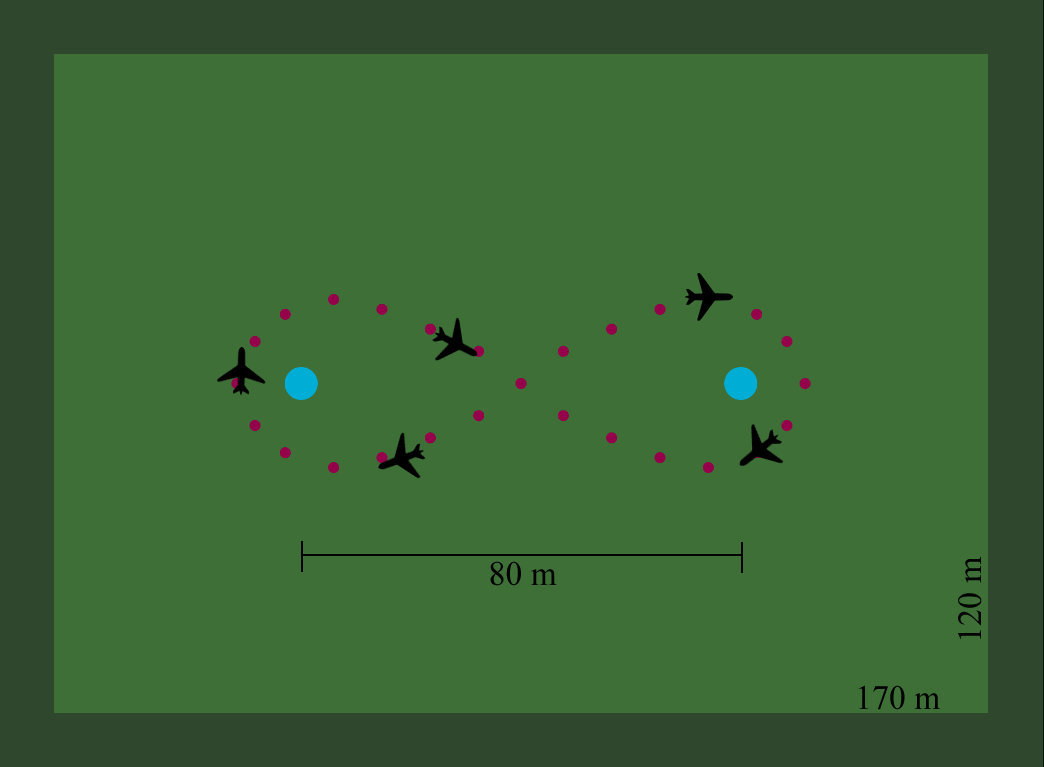
\includegraphics[width=1\textwidth]{osemka}
    \caption{Schemat misji samolotu na wyznaczonym obszarze.}
    \label{fig:osemka}
\end{figure}

Algorytm sterowania ma zostać wytrenowany na podstawie danych z przelotu pilota, który odpowiednią ilość razy wykona przelot treningowy. Zadaniem sztucznej inteligencji będzie skorelowanie zachowania pilota z sytuacją, w której znajduje się samolot. Następnie, w trybie autonomicznym, algorytm ma oszacować najbardziej prawdopodobne zachowanie pilota w danej chwili czasowej oraz bezpośrednio wykorzystać je do sterowania samolotem. 

Przygotowanie opisanego algorytmu wiąże się z koniecznością przygotowania szeregu rozwiązań, którymi są:
\begin{enumerate}
	\item Neuronowy algorytm sterowania.
	\item Środowisko treningowe sieci neuronowej.
	\item Oprogramowanie kontrolera.
	\item Elektroniczny moduł kontrolera.
	\item Samolot służący jako platforma treningowa.
	\item Stacja odbiorcza.
	\item Naziemne oprogramowanie.
	\item Pozostałe rozwiązania pozwalające na współpracę wszystkich wyżej wymienionych elementów.
\end{enumerate}

Poniższa praca zawiera opis wiedzy potrzebnej do zrozumienia opisu działań wykonywanych w części implementacyjnej, przegląd literatury naukowej i istniejących rozwiązań, opis procesu wdrożenia wymienionych powyżej elementów, a także omówienie rezultatu i podsumowanie wniosków.

\textbf{Uwaga}: określenie ``środowisko'' używane w poniższej pracy, w kontekście stworzonych programów, odnosi się do połączenia wszystkich systemów po stronie samolotu jak i stacji naziemnej. Warto również wspomnieć o wieloznaczności często używanego słowa ``model''. Model samolotu jest określeniem zdalnie sterowanego bezzałogowego statku powietrznego, którego wymiary nie przekraczają kilku metrów. Innym często padającym znaczeniem tego słowa jest odniesienie do modelu sztucznej inteligencji, który oznacza pewną konkretną instancję struktury danych wyniku nauczania maszynowego, w tym przypadku sieci neuronowej.

\clearpage
\section{Wstęp teoretyczny}

\subsection{Technika sterowania samolotem}
Problem sterowaniem trajektorią lotu samolotu jest dość nieoczywisty ze względu charakter sposobu utrzymania się takiego urządzenia w powietrzu. Przede wszystkim, do pokonania siły grawitacji wykorzystywana jest siła nośna wytwarzana na powierzchni skrzydeł. Jej źródłem jest różnica ciśnień nad i pod nimi, spowodowana różnymi prędkościami przepływu strugi powietrza od górnej i dolnej strony profilu lotniczego. Wartość generowanej siły nośnej jest proporcjonalna do różnicy tych prędkości, co w praktyce przekłada się na proporcjonalną zależność wartości siły nośnej do prędkości samolotu względem masy powietrza, w którym się porusza. Sytuację, w której samolot wytraca prędkość względem powietrza, co skutkuje utratą siły nośnej i w konsekwencji nagłym spadkiem i utratą sterowności nazywamy przeciągnięciem.

Sterowanie samolotem odbywa się przy pomocy elementów nazywanych powierzchniami sterowymi. Są to lotki umieszczone na skrzydłach oraz stery wysokości i kierunku znajdujące się na stateczniku. Osie rotacji według angielskiej notacji nazywane są \textit{roll}, \textit{pitch} oraz \textit{yaw}, jak zostało pokazane na rysunku \ref{fig:osie}. Poruszanie lotkami pozwala na wywołanie momentu działającego wzdłuż osi roll, co przekłada się na obrót wzdłuż niej, o ile pozwalają na to warunki. Analogicznie, moment w osi pitch wywołany jest przez ster wysokości, a w osi yaw - ster kierunku.

\begin{figure}[ht]
    \centering
    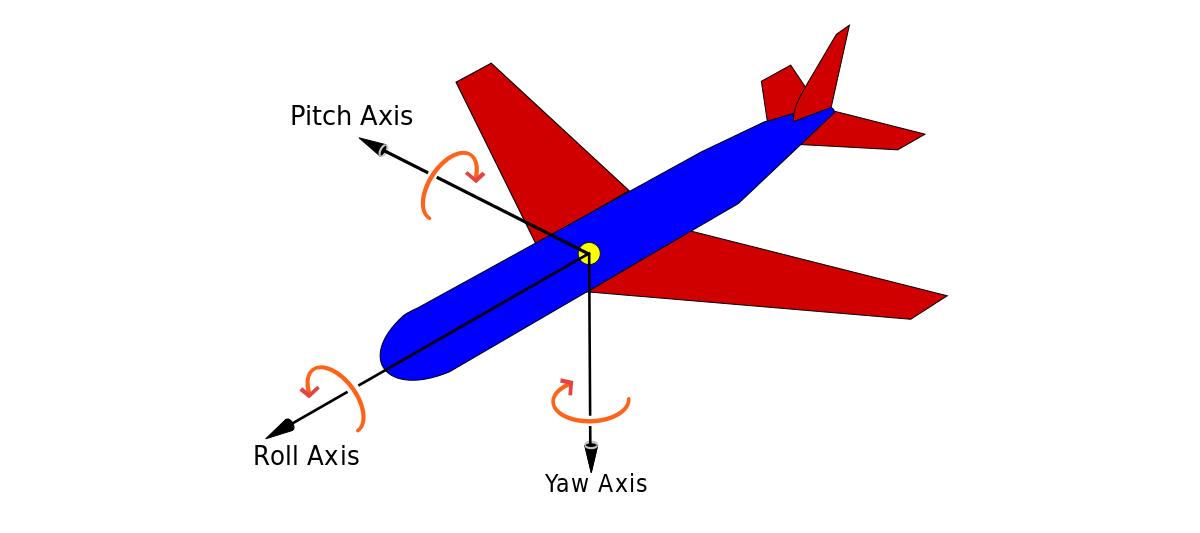
\includegraphics[width=1\textwidth]{osie}
    \caption{Osie rotacji samolotu.}
    \small Źródło: \url{en.wikipedia.org/wiki/Aircraft_principal_axes}
    \label{fig:osie}
\end{figure}

Należy jednak zaznaczyć, że w celu wykonania zakrętu samolot należy najpierw przekręcić używając lotek, następnie korygować trajektorię przy pomocy steru wysokości, a ster kierunku służy tylko do zmniejszenie promienia zakrętu i kontrowania wiatru bocznego.

\FloatBarrier
 
\subsection{Rozwiązania dostępne na rynku}
Na rynku dostępne są urządzenia spełniające definicję kontrolera do autonomicznego statku powietrznego - urządzenia te nadają się do wykorzystania zarówno w modelach samolotów jak i w wielowirnikowcach. Jednym z najpopularniejszych tego typu rozwiązań jest rodzina urządzeń Pixhawk. Jest to rozwiązaniem sprawdzone i często wykorzystywane nawet w zaawansowanych komercyjnych projektach. Innymi dostępnymi rozwiązaniami są urządzenia Mateksys czy CUAV pokazane na rysunku \ref{fig:kontrolery}.

Kontroler lotu jest urządzeniem zbierającym dane z różnych czujników, przede wszystkim IMU (czujnika orientacji), GPS/GNSS (czujnika położenia) czy rurki Pitota (czujnika względnej prędkości wiatru). Do modułu podłączany jest także odbiornik z aparatury RC, natomiast jego wyjściem są sygnały PWM do ustawienia odpowiednich powierzchni sterowych lub prędkości silników. 
Moduł kontrolera lotu może pracować w kilku trybach, z których najważniejszymi są:
\begin{enumerate}


	\item Tryb manualny - bezpośrednie przekazanie sygnału z odbiornika na wyjście sterowania. Tryb ten może być używany podczas startu i lądowania, oblocie samolotu lub w sytuacjach awaryjnych. Pełną kontrolę nad statkiem ma wtedy osoba trzymająca aparaturę.
	\item Tryb stabilizowany - rozszerzenie trybu manualnego - pilot ma wciąż kontrolę nad samolotem z poziomu aparatury, natomiast przy pomocy czujników znajdujących się na pokładzie kontroler stabilizuje lot, dzięki czemu latanie jest zdecydowanie ułatwione, zwłaszcza większymi modelami.
	\item Tryb autonomiczny - w tym trybie pojazd wykonuje zadaną misję, czyli przelot po kolejnych punktach na trasie. Podłączenie z aparaturą nie jest konieczne, a lot może się odbywać na bardzo długim dystansie. W przypadku zakończenia misji i braku dalszych poleceń samolot uruchomi procedurę RTL (return to landing) lub RTH (return to home) i zacznie zataczać okręgi nad wyznaczonym punktem na ustalonej, bezpiecznej wysokości.

\end{enumerate}
	
Dodatkowym zadaniem kontrolera lotu jest wysyłanie danych telemetrycznych w czasie rzeczywistym do stacji odbiorczej, co w praktyce przekłada się na umożliwienie podglądu pozycji i parametrów samolotu z poziomu laptopa oraz konfiguracja ustawień i wgrywanie nowych misji.

 \begin{figure}[ht]
    \centering
    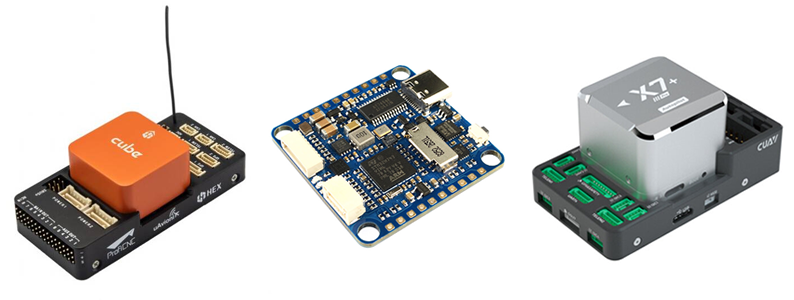
\includegraphics[width=1\textwidth]{kontrolery}
    \caption{Komenrcyjne kontrolery lotu: Pixhawk Cube Orange, Mateksys H743-SLIM, CUAV X7-PRO.}
    \small Źródła: \url{www.drony.net/the-orange-cube-standard-ads-b-proficnc-hex.html}, \url{www.mateksys.com/?portfolio=h743-slim}, \url{store.cuav.net/shop/x7-pro}
    \label{fig:kontrolery}
\end{figure}

Wspomniane urządzenia z rodziny Pixhawk czy CUAV są jednostkami, na których musi zostać uruchomione odpowiednie oprogramowanie. Odpowiada ono bezpośrednio za algorytmy wspomagania sterowania oraz lotów autonomicznych. Najczęściej wykorzystywanymi są ArduPilot oraz PX4. Oba te środowiska tworzone są na zasadzie open-source, a więc korzystanie z nich jest darmowe i ogólnodostępne. 

Do konfiguracji kontrolera lotu niezbędne jest oprogramowanie, które pozwoli na wprowadzenie zmian w ustawieniach zachowania samolotu w powietrzu, a także pozwoli przygotować i zarządzać przebiegiem autonomicznej misji, ponadto będzie w stanie przetworzyć i zwizualizować dane telemetryczne odbierane w czasie rzeczywistym. Najpopularniejszymi programami współpracującymi z przytoczonymi kontrolerami jest Mission Planner oraz QGroundControl.

\begin{figure}[ht]
    \centering
    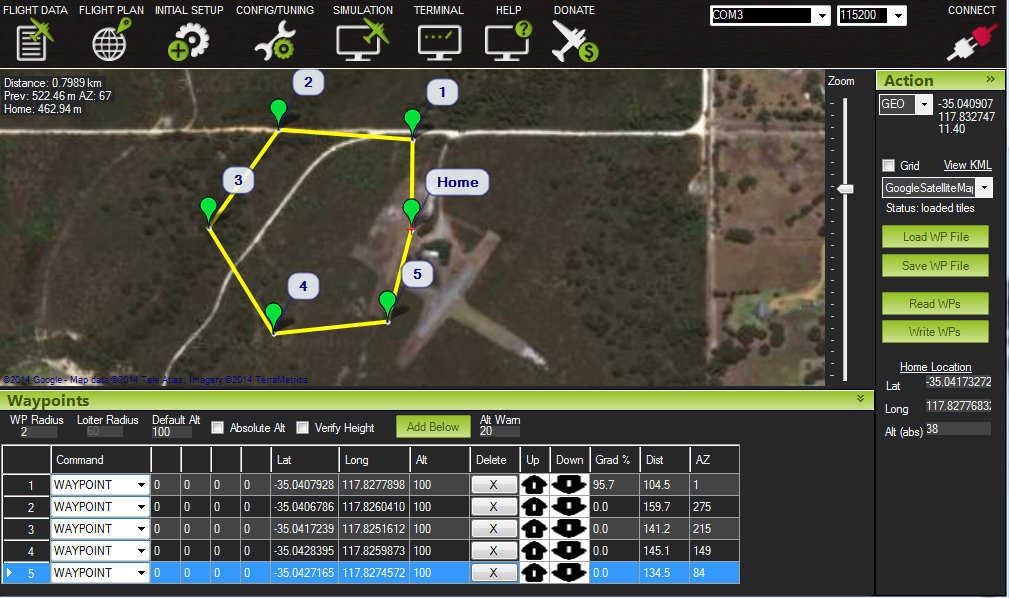
\includegraphics[width=1\textwidth]{missionplanner}
    \caption{Przygotowanie misji w programie Mission Planner.}
    \small Źródło: \url{ardupilot.org/planner}
    \label{fig:missionplanner}
\end{figure}

Przygotowanie misji w tych programach działa na zasadzie ustawienia pozycji oraz wysokości kolejnych punktów na trasie, zwanych waypointami, jak pokazano na rysunku \ref{fig:missionplanner}. W przypadku wielowirnikowców możliwe jest ustawienie trasy po dowolnej krzywej, z uwagi na możliwość sterowania nim w każdym kierunku i precyzyjne korygowanie trasy. Z kolei w samolotach takie sterowanie nie jest możliwe, dlatego pokonując trasę będą one dążyły do śledzenia linii łączącej środki kolejnych punktów. Warto zauważyć, że same waypointy nie są punktami, a okręgami o określonym promieniu. Po przekroczeniu granicy okręgu punkt uznawany jest za zaliczony, a samolot rozpoczyna manewr naprowadzający go na kolejny cel.
\FloatBarrier
\subsection{Przegląd literatury naukowej}
\clearpage
\section{Implementacja rozwiązania}
\subsection{Budowa modelu samolotu}
Charakterystyka pracy systemu lotu autonomicznego sprawia, że powinien  on zostać dostosowany do konkretnego modelu samolotu. Podczas początkowych testów używany był w tym celu samolot Multiplex EasyGlider 4, widoczny na zdjęciu \ref{fig:eg4}. Jest to komercyjny samolot o rozpiętości skrzydeł 1,8 metra, wykonany z Elaporu (polipropylen). Dzięki swoim parametrom aerodynamicznym możliwy jest nim stabilny lot przy stosunkowo niskiej prędkości przelotowej. Dodatkową zaletą jest jego wytrzymałość, co w przypadku modelu testowego jest istotne ze względu na możliwe niepowodzenia działania systemów pokładowych.

\begin{figure}[ht]
    \centering
    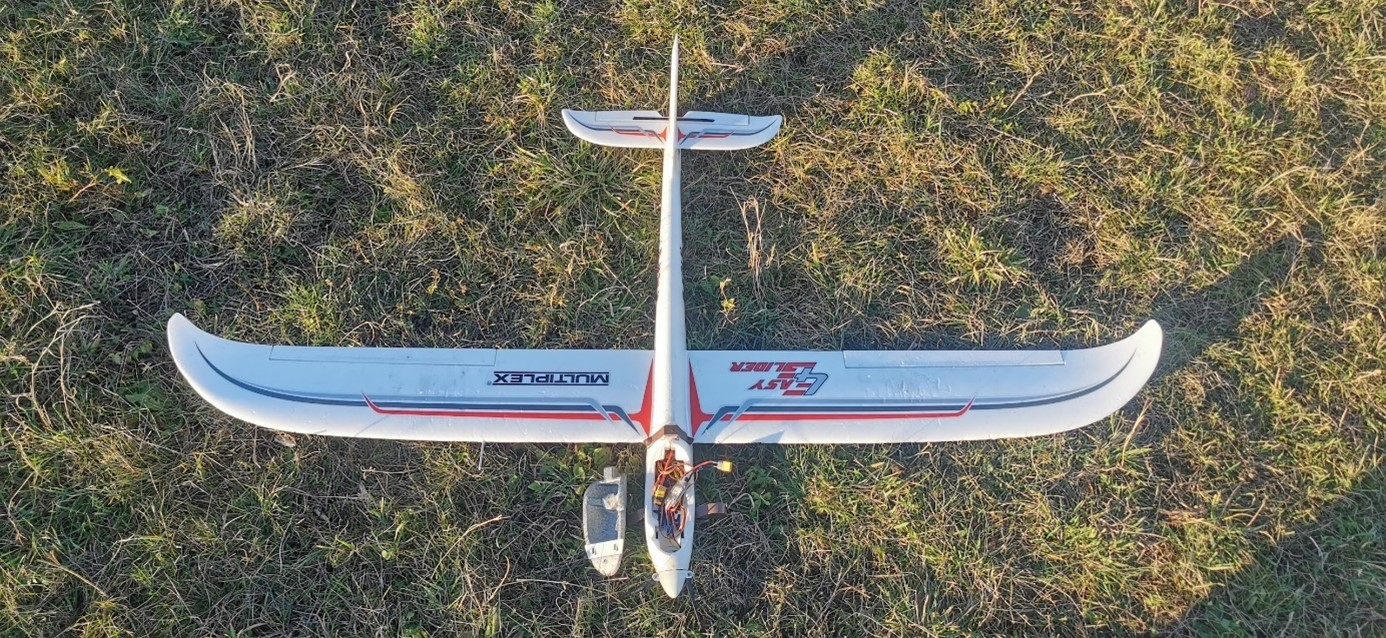
\includegraphics[width=1\textwidth]{budowa1}\\
    \caption{Samolot EasyGlider 4 wraz z modułem kontrolera lotu.}
    \label{fig:eg4}
\end{figure}

EasyGlider 4 nie jest jednak przystosowany do przenoszenia większej ilości urządzeń podkładowych poza odbiornikiem i baterią. Jego mocno ograniczona objętość kadłuba sprawiała, że wymiana baterii wiąże się z każdorazowym rozłączeniem kabli oraz wyjęciem większości elektroniki. Taki proces naraża na uszkodzenie elementy na płytce prototypowej, a także zajmuje dużo czasu, zwłaszcza w warunkach polowych. Samolot posłużył do ogromnej ilości testów systemów oraz elektroniki, jednak zgodnie z założeniem projektu, docelowo używany samolot miał być dedykowany do modułu kontrolera. Konieczne więc było zaprojektowanie i przygotowanie modelu spełniającego odpowiednie założenia wytrzymałościowe i aerodynamiczne. Jego projekt został wykonany w programie XFLR5 i pokazany został na rysunku \ref{fig:xflr}.

 \begin{figure}[ht]
    \centering
    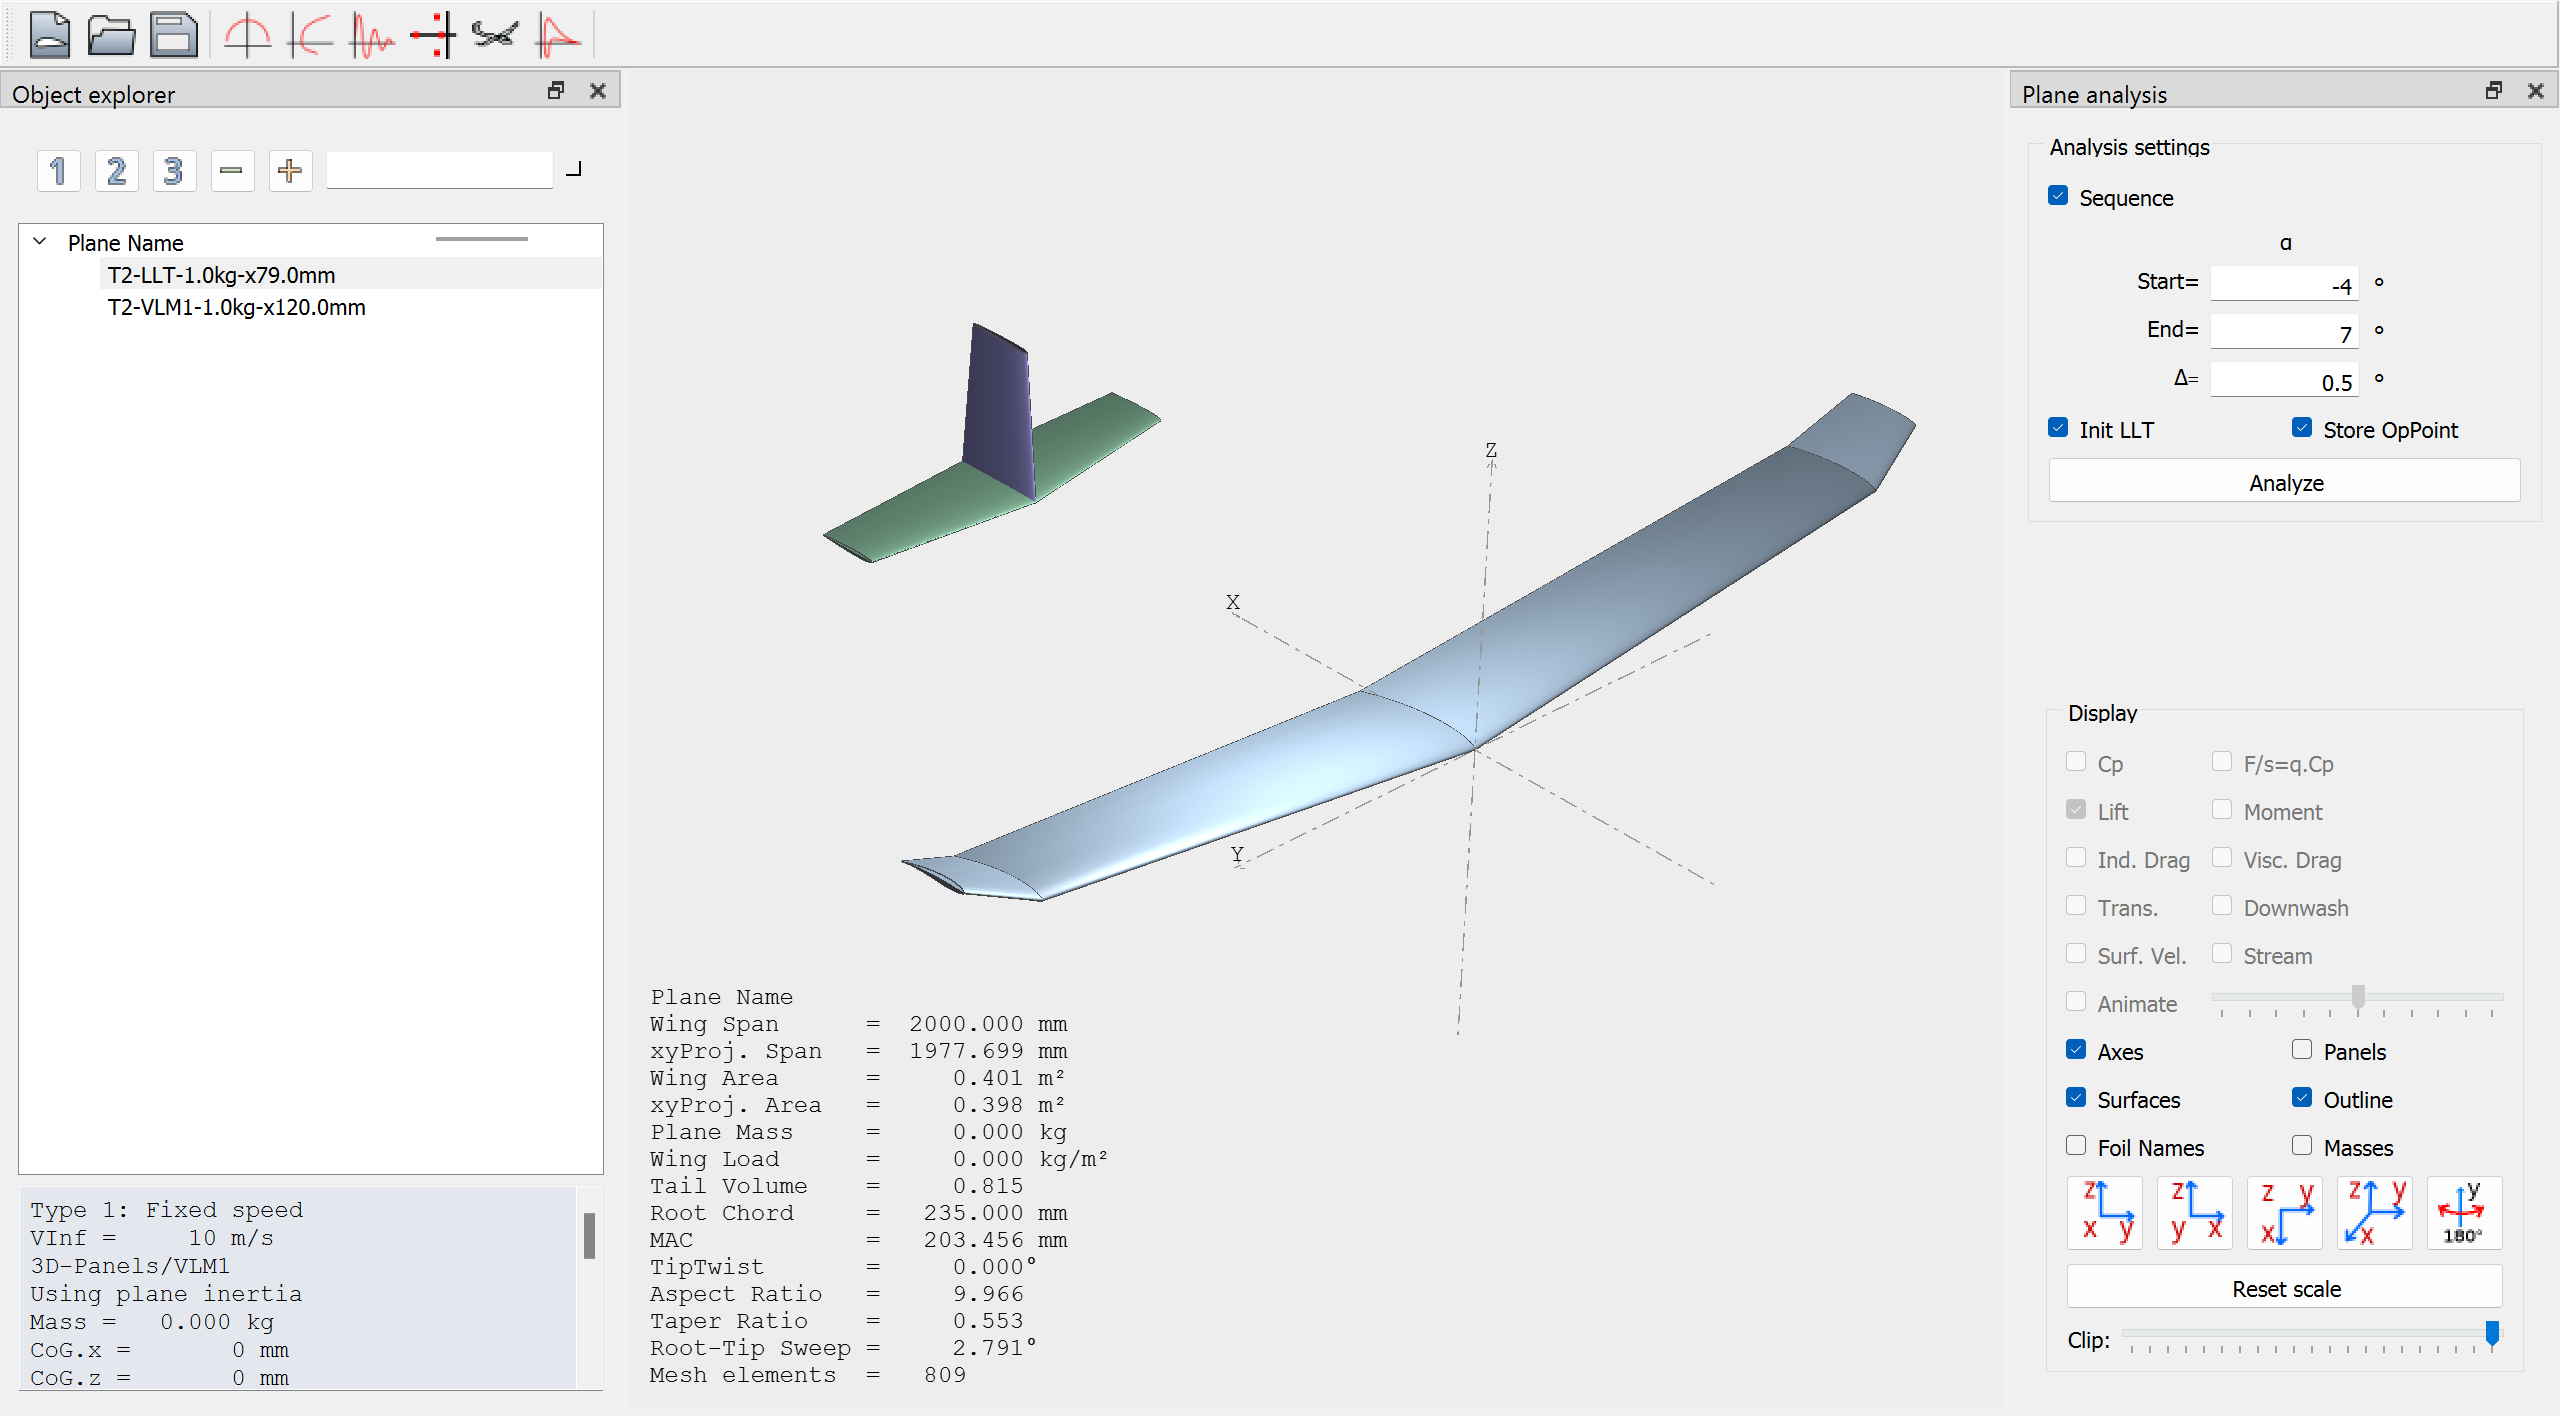
\includegraphics[width=1\textwidth]{xflr}
    \caption{Ekran główny programu XFLR5 z projektem samolotu.}
    \label{fig:xflr}
\end{figure}

Jako profil lotniczy skrzydła wybrany został FX 60-100, widniejący na grafice \ref{fig:fx60}. Jest on stosunkowo gruby oraz wklęsły w swojej dolnej części, co przekłada się na zwiększone opory powietrza oraz większą siłę nośną, przy równoczesnej niższej prędkości przelotowej. Na końcach skrzydeł znajdują się uszka o tym samym profilu. Kąt wzniosu skrzydeł wynosi 5\textdegree na każdą stronę, natomiast uszka wzniesione są o dodatkowe 15\textdegree.  Całkowita rozpiętość skrzydeł wynosi 2 metry.

 \begin{figure}[ht]
    \centering
    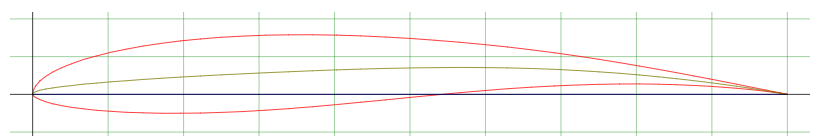
\includegraphics[width=1\textwidth]{fx60}
    \caption{Profil lotniczy FX60-100.}
    \small Źródło: \url{airfoiltools.com/airfoil/details?airfoil=fx60100-il}
    \label{fig:fx60}
\end{figure}

Statecznik poziomy i pionowy posiadają profil lotniczy NACA 0008 (grafika \ref{fig:naca}), który jest profilem symetrycznym. Statecznik jest stosunkowo duży, co zapewnia dodatkową stabilizację podczas lotu. Znajduję się on 90 cm od początku krawędzi natarcia skrzydła głównego.

 \begin{figure}[ht]
    \centering
    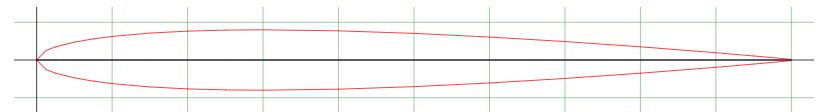
\includegraphics[width=1\textwidth]{naca0008}
    \caption{Profil lotniczy NACA 0008.}
    \small Źródło: \url{airfoiltools.com/airfoil/details?airfoil=naca0008-il}
    \label{fig:naca}
\end{figure}

Dzięki przeprowadzeniu analizy projektu w programie XFLR możliwe jest uzyskanie parametrów aerodynamicznych samolotu. Na wykresach \ref{fig:wykresy} obserwować można cztery zależności. Wykres w lewym górnym informuje o zależności prędkości w pionie i poziome, wykres w prawym góry rogu podaje zależność prędkości przelotowej od kąta natarcia. Zależność Cm(Alfa) na lewym dolnym wykresie informuje o stabilności samolotu, która będzie optymalna w punkcie przecięcia z osią X. Z wykresu w prawym dolnym rogu odczytać można zależność doskonałości aerodynamicznej od kąta natarcia skrzydeł. Doskonałość jest dystansem jaki przeszybuje samolot tracąc przy tym metr wysokości. 

Na podstawie wykresów możliwe jest określenie odpowiedniego kąta natarcia skrzydeł jako kąta 2,5\textdegree. Prędkość przelotowa wynosi wtedy 7m/s, a współczynnik doskonałości jest równy 18.

\begin{figure}[ht]
    \centering
    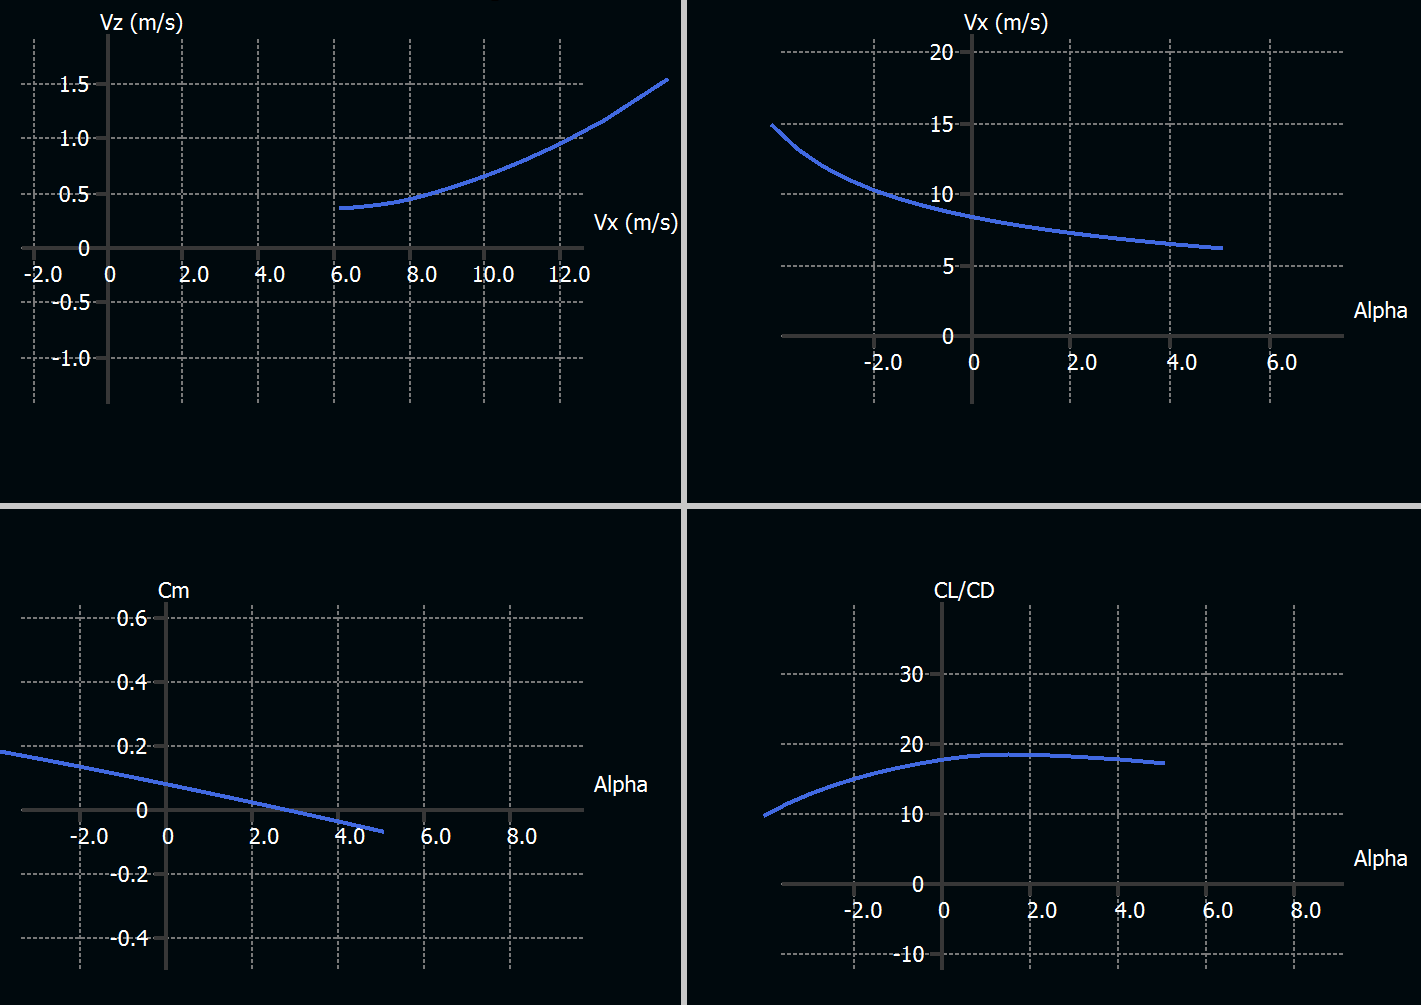
\includegraphics[width=1\textwidth]{wykresy}
    \caption{Wyniki analizy projektu samolotu w programie XFLR5.}
    \label{fig:wykresy}
\end{figure}

\FloatBarrier
\paragraph{Wytworzenie elementów kompozytowych}\mbox{}

Po zakończeniu procesu projektowania, pierwszym niezbędnym elementem do przygotowania są bryty na skrzydła oraz statecznik wykonane z polistyrenu ekstrudowanego, potocznie nazywanego styrodurem. Ze styrodurowej płyty, na ploterze termicznym, za pomocą gorącego drutu wycinany jest obrys profili przez dwie oddalone od siebie karetki, co pokazuje zdjęcie \ref{fig:ploter}. W ten sposób możliwe jest otrzymanie dokładnej geometrii zaprojektowanego skrzydła, a równocześnie form negatywowych, które zostaną wykorzystane później w procesie laminowania.

\begin{figure}[ht]
    \centering
    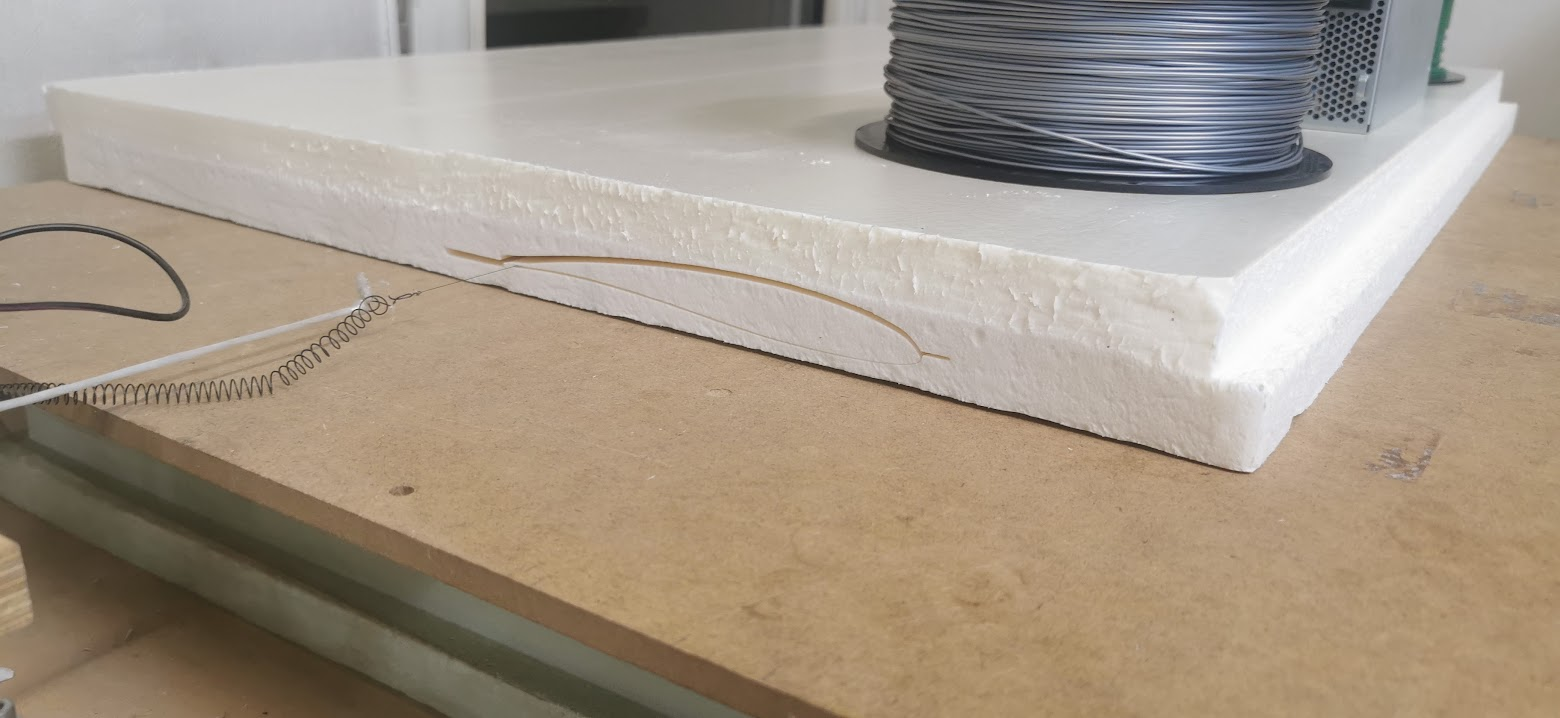
\includegraphics[width=1\textwidth]{budowa5}
    \caption{Proces wycinania brytów przy pomocy plotera termicznego.}
    \label{fig:ploter}
\end{figure}
 
W analogiczny sposób wycięte zostały bryty na uszka oraz elementy statecznika. Przed dalszymi działaniami skrzydła muszą zostać okablowane, czyli przewody doprowadzające zasilanie i sygnały do różnych elementów muszą zostać umieszczone w styrodurze w taki sposób, aby nie zaburzały powierzchni profilu lotniczego. W prawym skrzydle (zdjęcie \ref{fig:okablowane}) widoczne są przewody do czujnika rurki Pitota, modułu ogniw fotowoltaicznych oraz do serwomechanizmu poruszającego lotką.

 \begin{figure}[ht]
    \centering
    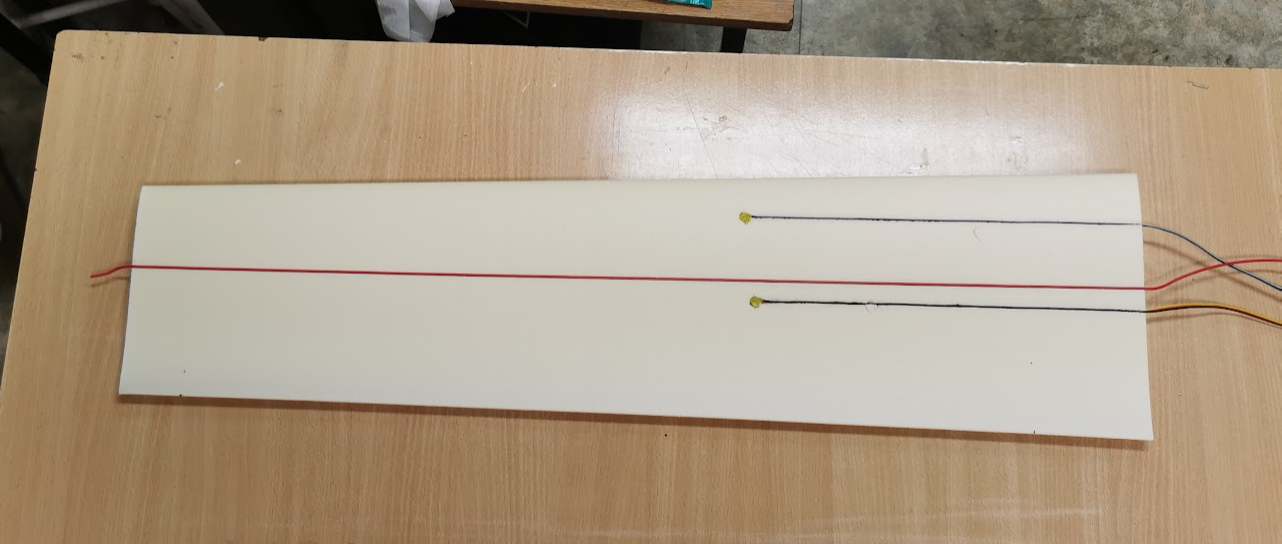
\includegraphics[width=1\textwidth]{okablowany}
    \caption{Okablowane prawe skrzydło, widok na jego dolą stronę.}
    \label{fig:okablowane}
\end{figure}

Same ogniwa fotowoltaiczne zostały uprzednio zalaminowane przy pomocy metody opracowanej przez zespół AGH Solar Plane, która pozwala na przylutowanie do siebie szeregu ogniw, a następnie zabezpieczenie ich przy pomocy folii od górnej strony oraz włókna szklanego od dołu. Dzięki temu możliwe jest wykorzystanie takiego modułu w procesie laminowania skrzydeł. Zapewnia to możliwość ich późniejszego dostosowania do kształtu skrzydła bez znaczącego spadku sprawności. Na zdjęciu \ref{fig:laminowanie} widoczny jest szereg ogniw fotowoltaicznych na folii Mylar, przykrytych warstwą tkaniny szklanej, gotowy do dalszego procesu laminowania.

 \begin{figure}[ht]
    \centering
    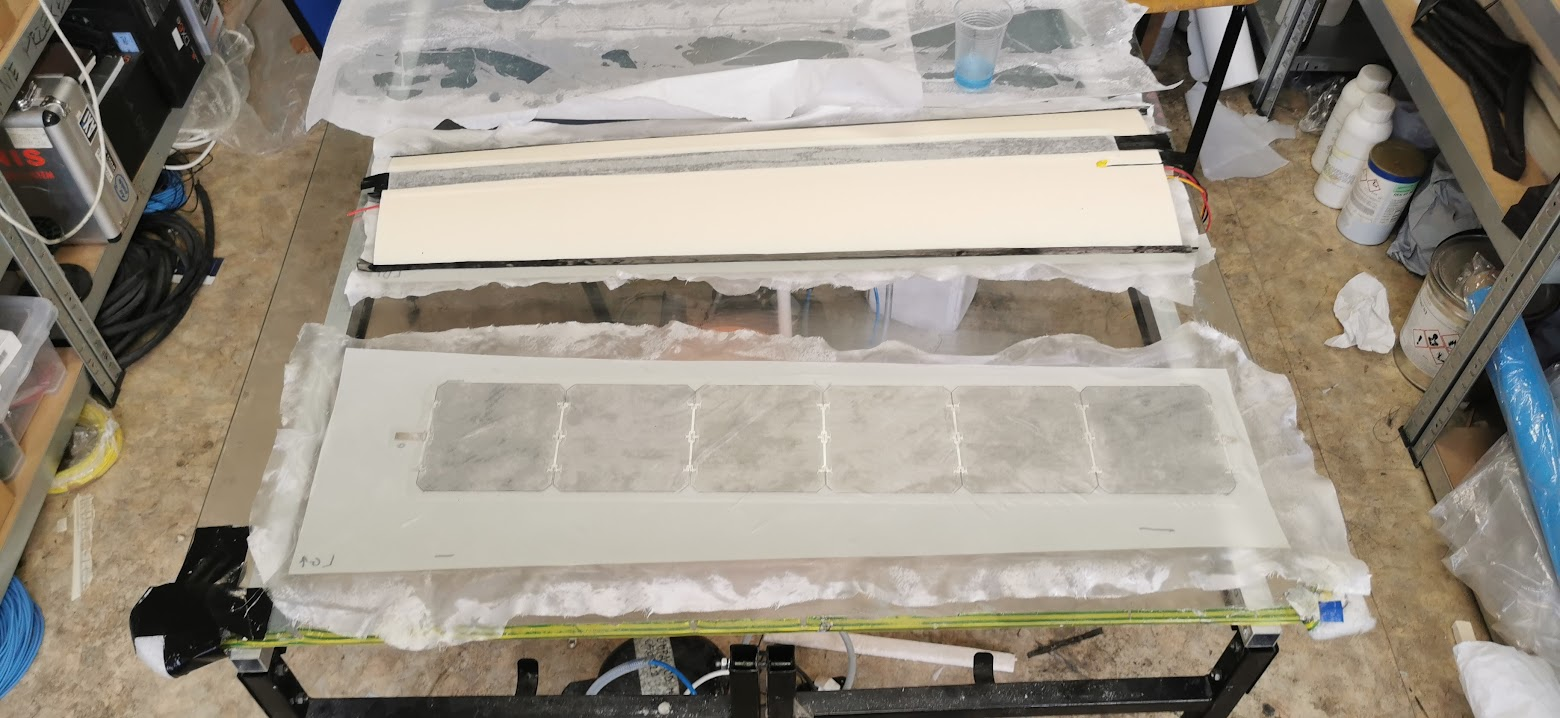
\includegraphics[width=1\textwidth]{budowa7}
    \caption{Przygotowanie instalacji fotowoltaicznej podczas laminowania skrzydła.}
    \label{fig:laminowanie}
\end{figure}

Skrzydła zyskują swój ostateczną formę w procesie laminowania. Polega ona na odpowiednim nałożeniu warstw laminatu na bryt i nasączeniu ich żywicą epoksydową. Z uwagi na instalację fotowoltaiczną umieszczoną na skrzydłach nie jest możliwe wykorzystanie laminatu z włókna węglowego, ponieważ istnieje bardzo duże ryzyko zwarcia instalacji na całej jej długości - przez zabezpieczającą warstwę tkaniny szklanej przebić się mogą pojedyncze włókna węglowe, będące bardzo dobrymi przewodnikami energii elektrycznej. Jako laminat wykorzystane więc zostały dwie warstwy tkaniny szklanej o gramaturze 48 g/m2 na każdą powierzchnię. Węglowy rowing został jedynie wykorzystany jako wzmocnienie krawędzi spływu, natomiast krawędź natarcia oraz dźwigar zostały wykonane z taśmy węglowej o szerokości 20 mm (na dźwigarze znajdują się dwie warstwy). Na gotowy laminat zostaje położona folia Mylar, która pozwala odbić idealnie gładką powierzchnię. Tak przygotowane bryty laminaty są następnie umieszczane w worku próżniowym, z którego przy pomocy pompy usuwane jest powietrze do ciśnienia -400 mbar względem atmosfery. Ciśnienie to jest stosunkowo wysokie, w tego typu procesach częściej spotykane jest uzyskanie próżni rzędu -800 do -900 mbar, które nie zostało wykorzystane z uwagi na ryzyko uszkodzenia instalacji fotowoltaicznej.

Dzięki zastosowaniu próżni uzyskany jest bardzo duży, równomierny nacisk na całą powierzchnię brytu. Z uwagi na wypukło-wklęsły profil lotniczy skrzydła konieczne jest umieszczenie brytów w negatywowej formie, ponieważ worek poróżniony może mocno naciągnąć styrodur. Na koniec formy zostały przyciśnięte ciężkimi przedmiotami, jak zaobserwować można na zdjęciu \ref{fig:schniecie}. Czas schnięcia zastosowanej żywicy epoksydowej L285 wraz z utwardzaczem H287 wynosi około 24 godziny, dopiero po tym czasie prace mogą być kontynuowane.

 \begin{figure}[ht]
    \centering
    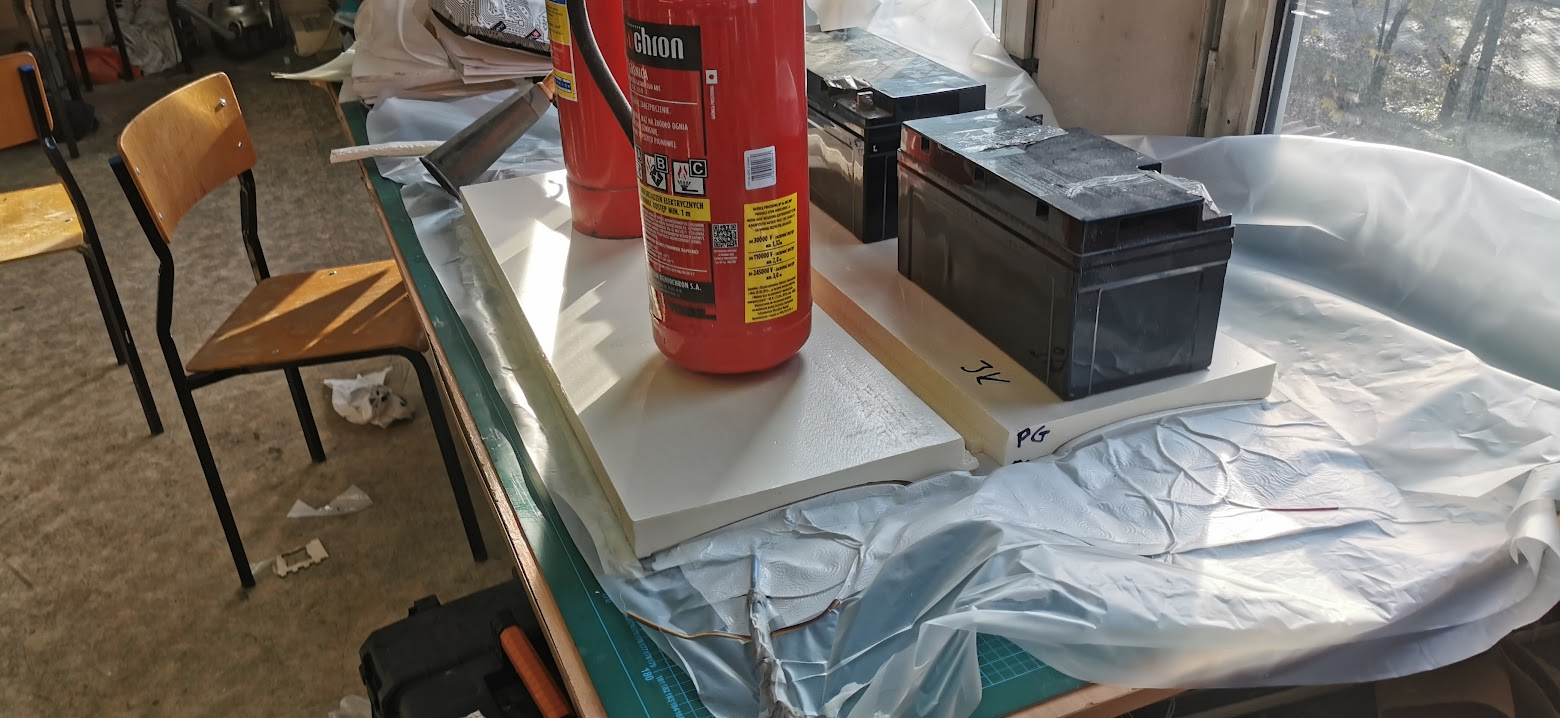
\includegraphics[width=1\textwidth]{budowa9}
    \caption{Skrzydła umieszczone w formach negatywowych i worku próżniowym w trakcie schnięcia.}
    \label{fig:schniecie}
\end{figure}

W analogiczny sposób zalaminowane zostały uszka oraz elementy statecznika. Przy okazji tego procesu wzmocniono krawędzie natarcia i spływu skrzydeł dodatkową warstwą włókien węglowych. Finalnym rezultatem procesu laminowania są widoczne na zdjęciu \ref{fig:kompozytki} elementy.

 \begin{figure}[ht]
    \centering
    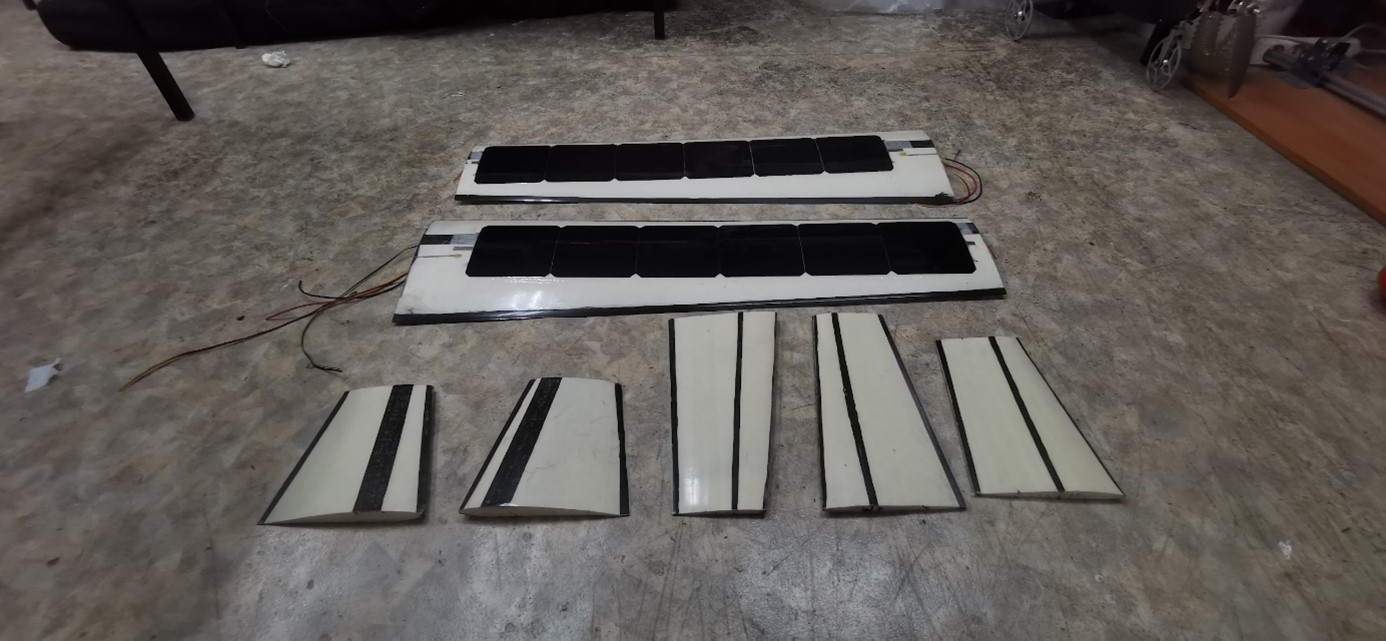
\includegraphics[width=1\textwidth]{budowa11}
    \caption{Elementy powstałe w wyniku procesu laminowania.}
    \label{fig:kompozytki}
\end{figure}

\FloatBarrier
\paragraph{Łączenie elementów}\mbox{}

Kolejnym etapem było połączenie skrzydeł oraz doklejenie do nich uszek. Efekt ten został osiągnięty przy pomocy kleju żywicznego Poxipol oraz wzmocnieniu połączeń fragmentami dwukierunkowej tkaniny węglowej. Elementy statecznika także zostały sklejone przy pomocy kleju Poxipol. Całość została umieszczona na rurze węglowej o długości 1 m i średnicy 20 mm. Gotowe elementy widoczne są na zdjęciu \ref{fig:sklejone}.

 \begin{figure}[ht]
    \centering
    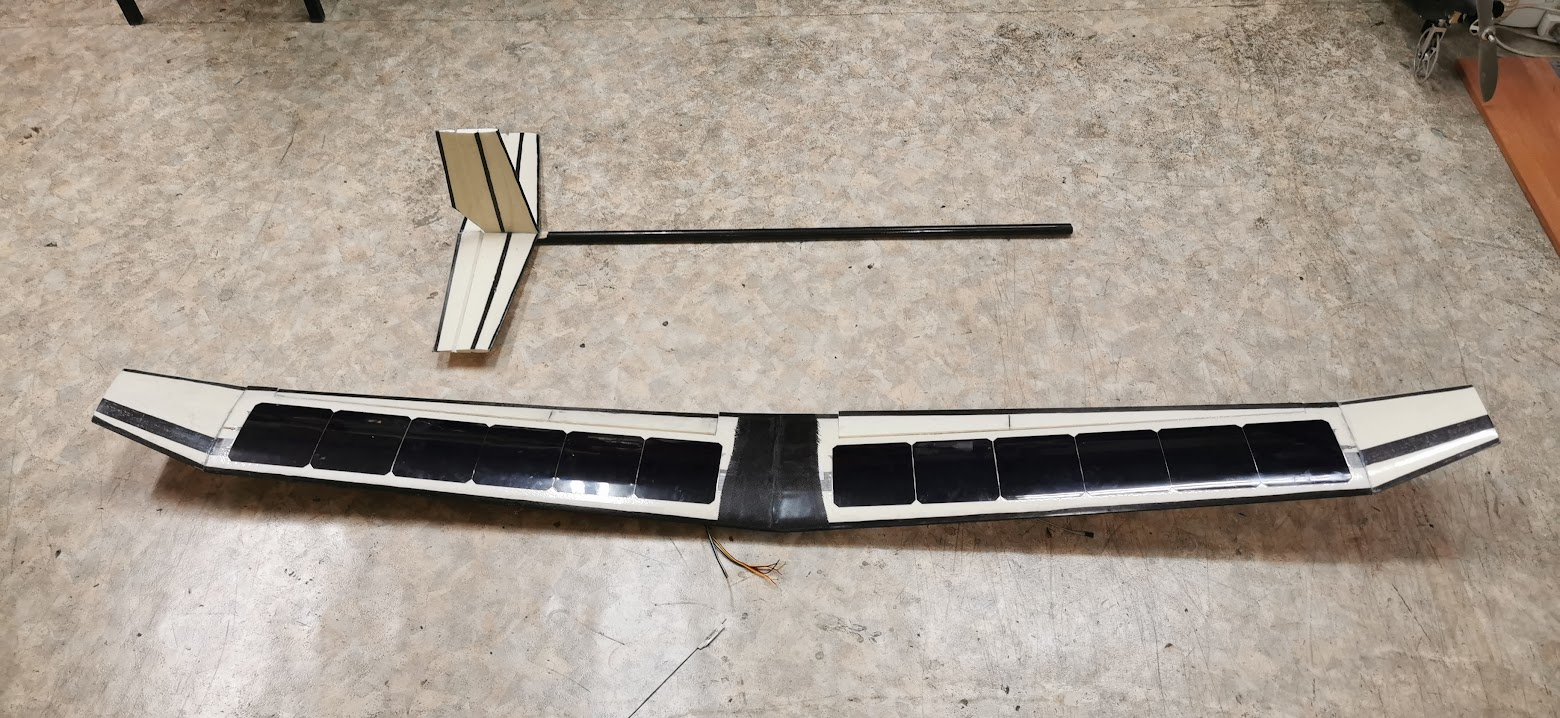
\includegraphics[width=1\textwidth]{budowa13}
    \caption{Połączone skrzydła oraz sklejony statecznik wraz z rurą węglową.}
    \label{fig:sklejone}
\end{figure}

Ostatnim niezbędnym laminowanym elementem była podstawka pod skrzydła, umożliwiająca uzyskanie kąta zaklinowania skrzydeł oraz ich systemu mocowania. Podstawka została zaprojektowana w programie Fusion 360, wyfrezowana na urządzeniu CNC i finalnie zalaminowana jedną warstwą dwukierunkowej tkaniny węglowej. Jak widać na zdjęciu \ref{fig:podstawka} jej kształt jest dopasowana do dolnej powierzchni centralnej części skrzydeł. Na środku przygotowane zostały otwory na kable idące do kadłuba.

 \begin{figure}[ht]
    \centering
    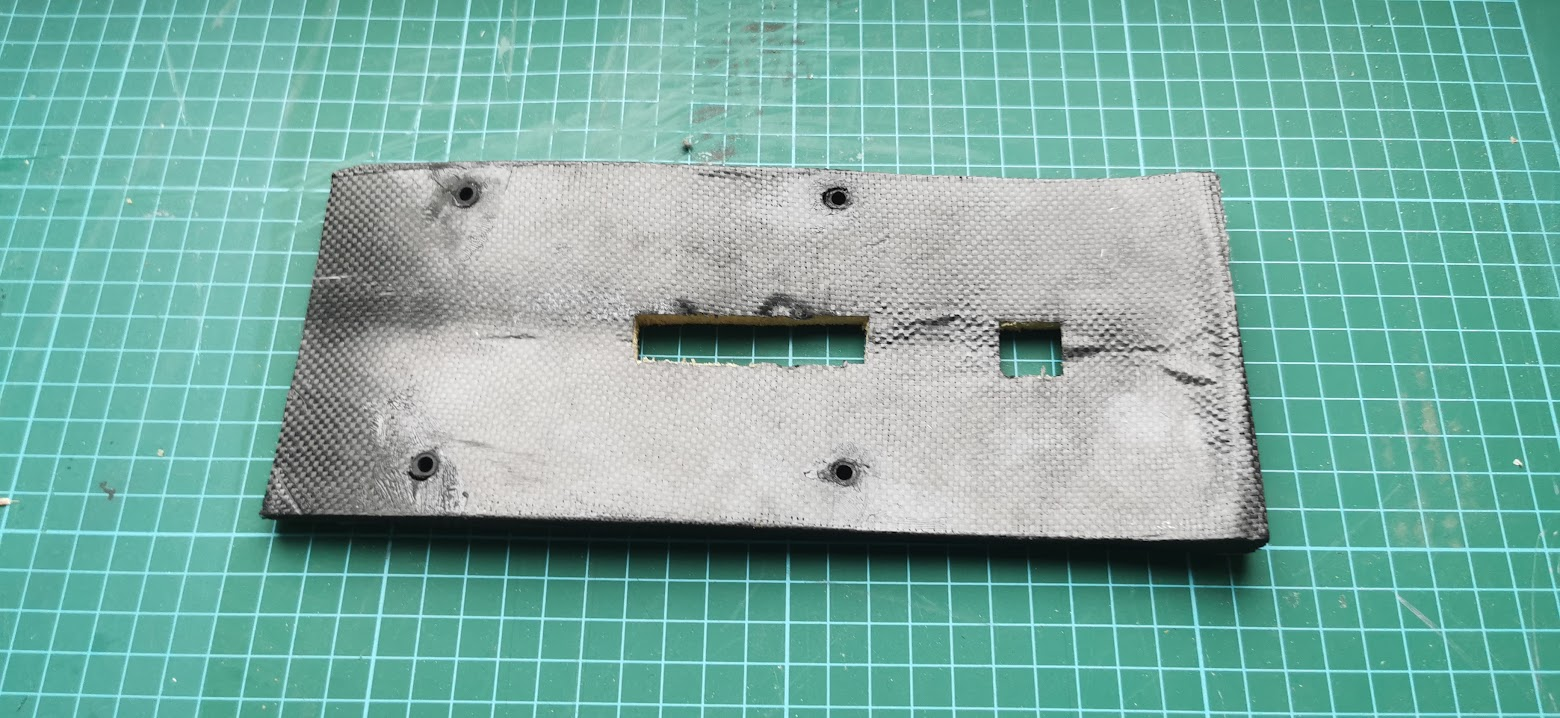
\includegraphics[width=1\textwidth]{podstawka}
    \caption{Podstawka pod skrzydła.}
    \label{fig:podstawka}
\end{figure}

\FloatBarrier
\paragraph{Kadłub}\mbox{}

Szkielet kadłuba został wykonany z listewek sosnowych sklejonych ze sobą klejem cyjanoakrylowym, jak widać na zdjęciu \ref{fig:szkielet}. Kadłub jest przyklejony do rury ogonowej, pod podstawką pod skrzydła znajduje się dodatkowo wzmocniona sklejka. Wnętrze kadłuba zostało rozplanowane w taki sposób, aby umożliwić jak najwygodniejszy dostęp do modułu kontrolera oraz baterii. W skrzydłach oraz w podstawce umieszczono węglowe tulejki, w które wkładane są śruby mocujące M4, łączące skrzydła z kadłuba. 

\begin{figure}[ht]
    \centering
    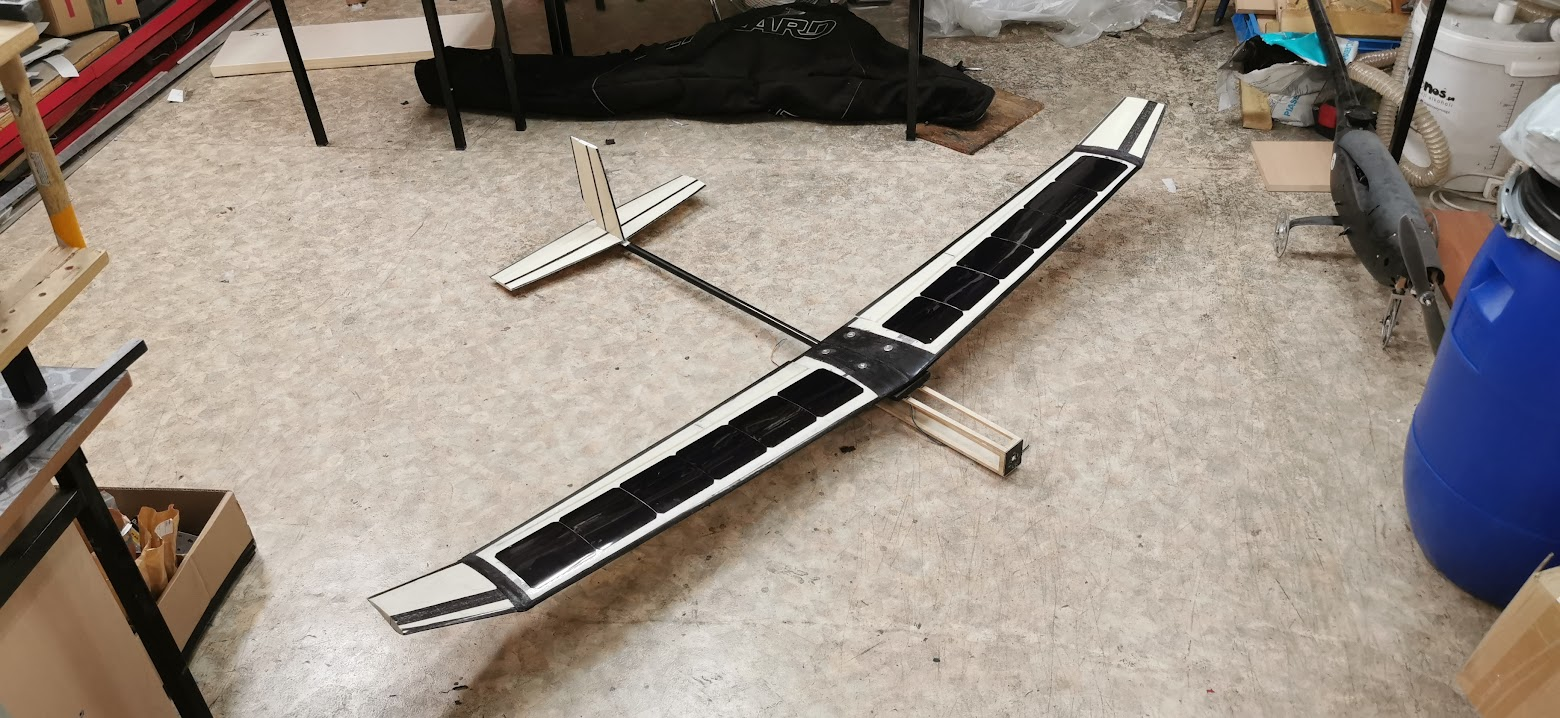
\includegraphics[width=1\textwidth]{szkielet}
    \caption{Złożony samolot z gotowym szkieletem kadłuba.}
    \label{fig:szkielet}
\end{figure}

Stery kierunku i wysokości obsługiwane są przy pomocy serwomechanizmów umieszczonych w kadłubie oraz bowdenów umieszczonych wzdłuż rury ogonowej, co pokazano na zdjęciu \ref{fig:tyl}. We wszystkie powierzchnie sterowe wklejone zostały wykonane z płyty węglowej orczyki prowadzące. 

\begin{figure}[ht]
    \centering
    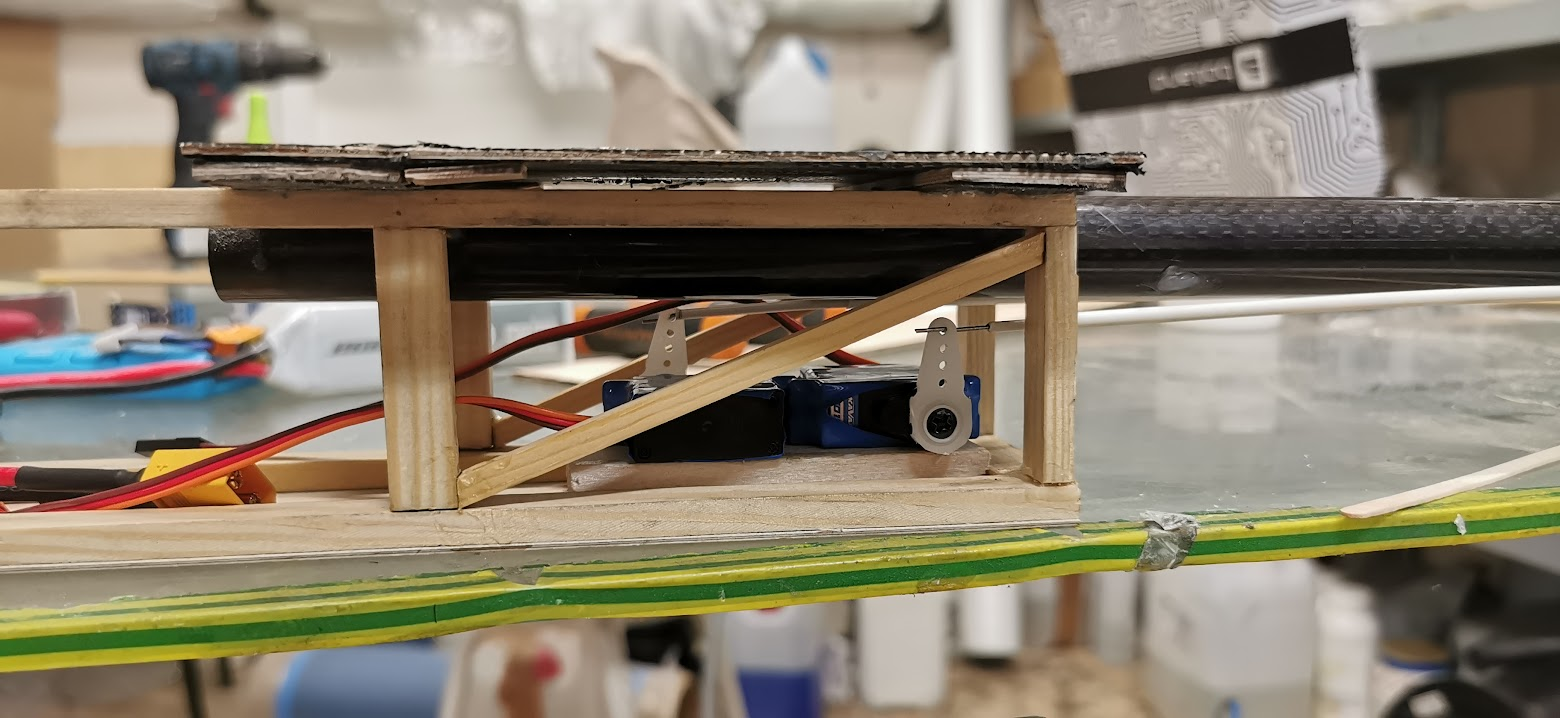
\includegraphics[width=1\textwidth]{tyl}
    \caption{Tylna część kadłuba - miesce mocowania skrzydeł oraz serwomechnizmy wraz z bowdenami do sterów kierunku i wysokości.}
    \label{fig:tyl}
\end{figure}

Po umieszczeniu całej elektroniki podkładowej szkielet kadłuba wzmocniono i zabezpieczono balsą modelarską. Przewidziana została możliwość szybkiego dostępu do kontrolera jak i do baterii przy pomocy umieszczonych na zawiasach zamknięciach, zamykanych za pomocą śruby M3, jak widać na zdjęciu \ref{fig:przod}. Antena GPS umieszczana jest na specjalnej podstawce za pomocą rzepa.

\begin{figure}[ht]
    \centering
    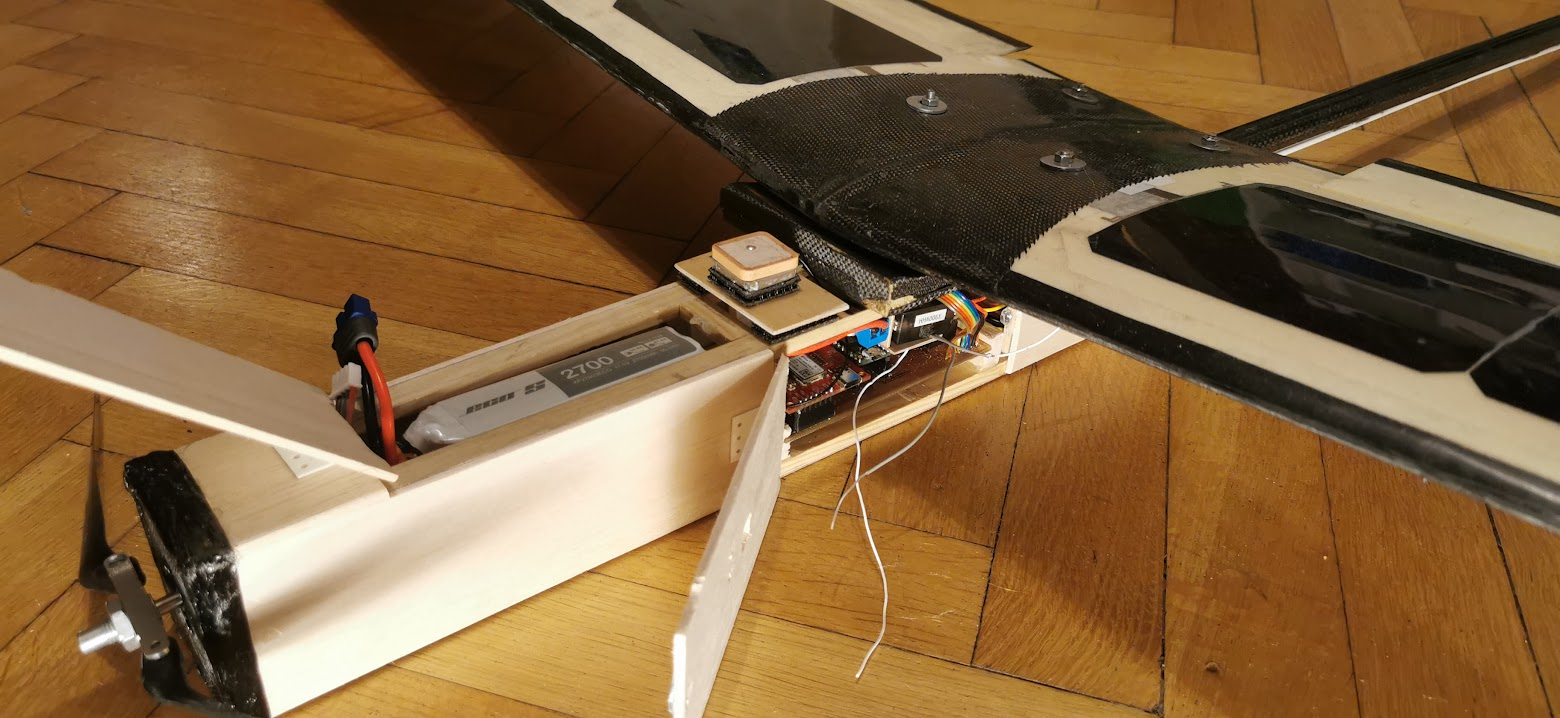
\includegraphics[width=1\textwidth]{przod}
    \caption{Przednia część kadłuba - zamknięcia osłaniające elektronikę i akumulator.}
    \label{fig:przod}
\end{figure}

\FloatBarrier
\paragraph{Złożenie samolotu}\mbox{}

Po złożeniu samolotu jego rozpiętość skrzydeł jest równa 204 cm, długość 130 cm a waga razem z akumulatorem wynosi około 1500 gramów. Do transportu możliwe jest odkręcenie skrzydeł i późniejsze ich ponowne przykręcenie - cała operacja, razem z podłączeniem wtyczek, trwa zaledwie kilka minut. 

Na zdjęciach widoczny jest złożony i uruchomiony samolot w trakcie pierwszego oblotu zaraz przed startem (zdjęcie \ref{fig:gotowy}) oraz po kilku pierwszych udanych lądowaniach (zdjęcie \ref{fig:lataxd}). Samolot został nazwany ``Dodo'' na cześć wymarłego ptaka nielota. 

\begin{figure}[ht]
    \centering
    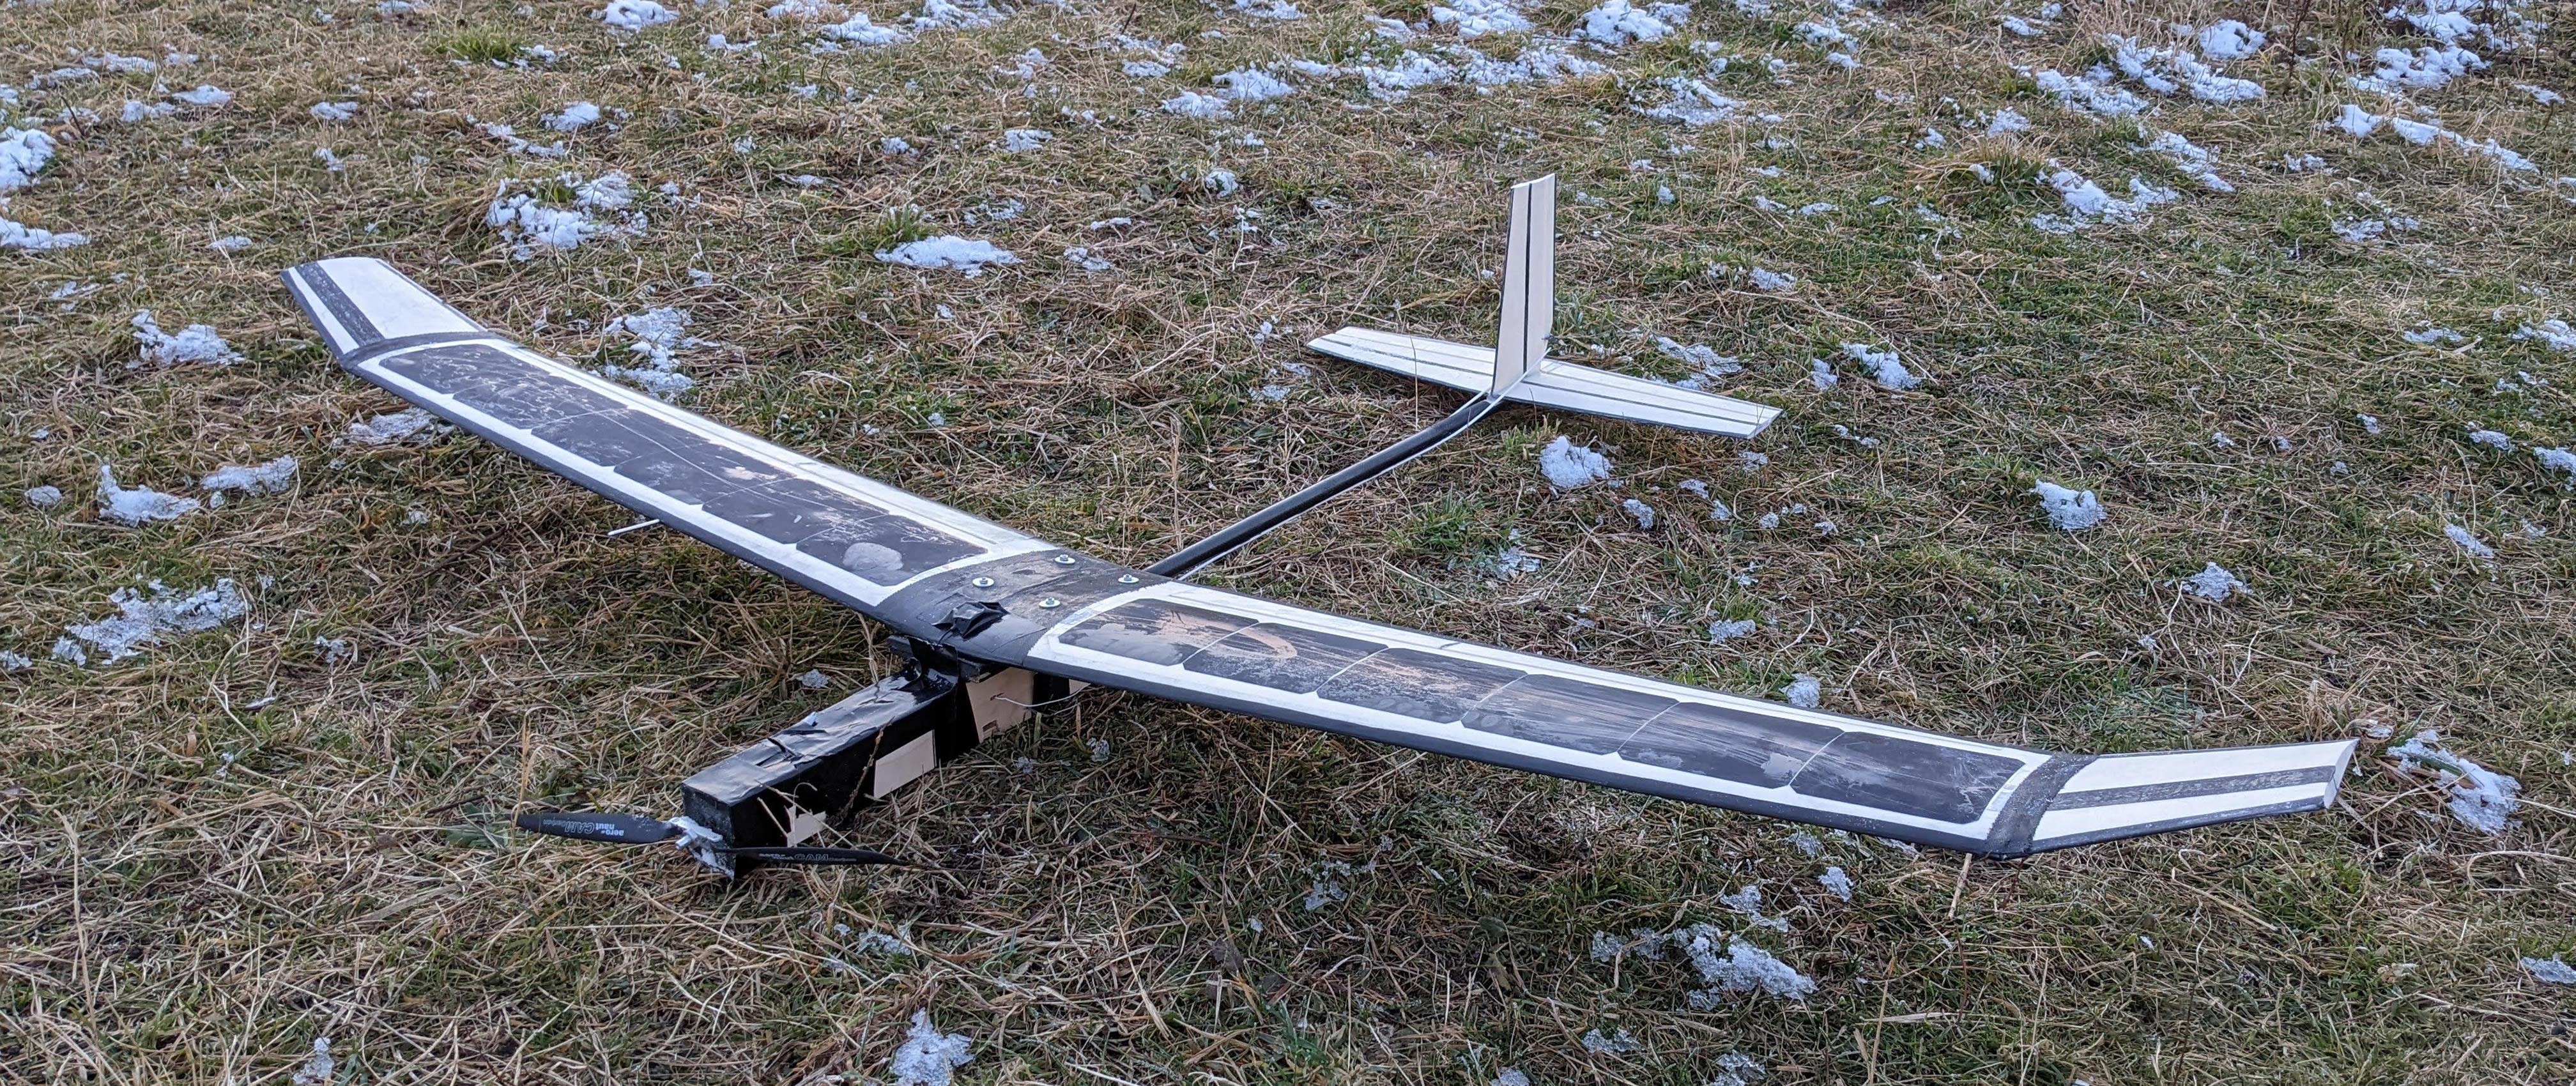
\includegraphics[width=1\textwidth]{dolotu}
    \caption{Złożony samolot przed pierwszym oblotem.}
    \label{fig:gotowy}
\end{figure}

\begin{figure}[ht]
    \centering
    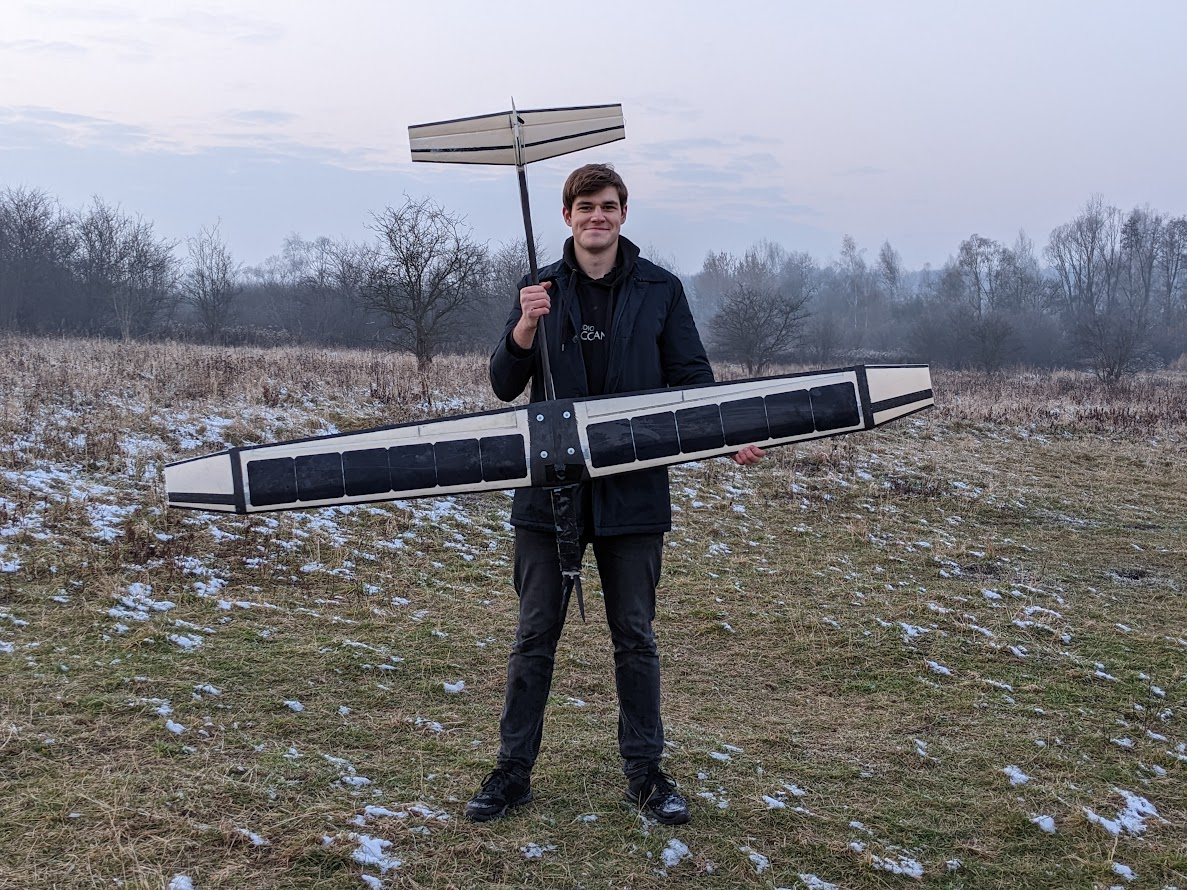
\includegraphics[width=1\textwidth]{budowa16}
    \caption{``Dodo'' po pierwszych lotach w rękach autora projektu.}
    \small Zdjęcie: inż. Andrzej Rusinowski
    \label{fig:lataxd}
\end{figure}

 \FloatBarrier
\subsection{Moduł instalacji fotowoltaicznej}
Prace nad kontrolerem opartym o sieć neuronową wymagają zebrania ogromnej ilości danych oraz obserwacji zachowania podczas lotu, co przekłada się na konieczność utrzymania go w powietrzu tak długo, jak to możliwe - każde lądowanie, wymiana baterii i kalibracja zajmuje bardzo cenne minuty podczas wyjazdu na testy. Aby zmaksymalizować czas samolotu w powietrzu, na jego skrzydłach umieszczona została instalacja fotowoltaiczna, która wspomaga zasilanie z baterii, a nawet pozwala ją częściowo naładować.

\begin{figure}[ht]
    \centering
    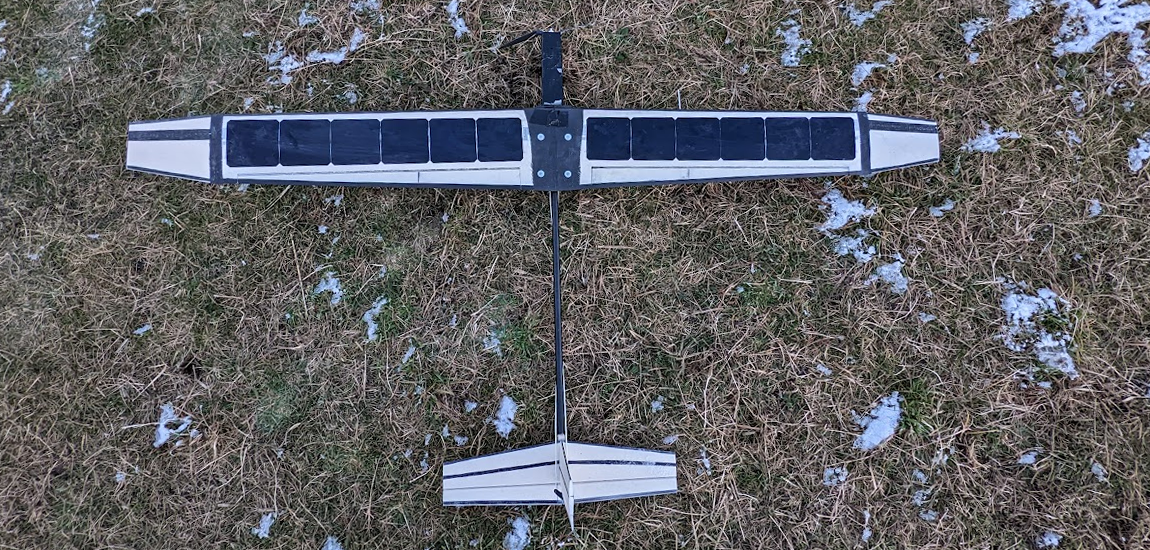
\includegraphics[width=1\textwidth]{panelki}
    \caption{Widok na instalację fotowoltaiczną umieszczona na samolocie.}
    \label{fig:panelki}
\end{figure}

Jak widać na zdjęciu \ref{fig:panelki}, instalacja składa się z 12 ogniw SunPower gen. 4 (wymiary 125 mm na 125 mm), każde o znamionowej mocy 3,6 W, działające przy napięciu maksymalnym 0,6 V. Zostały one wybrane ze względu na wysoką sprawność sięgająca nawet 23\%,  dodatkowo możliwe jest ich kupienie w czystej, niezabezpieczonej formie. Pozwala to na umieszczenie ich na skrzydłach ze względu na grubość rzędu dziesiątej części milimetra oraz giętkość pozwalającą na dopasowanie do profilu lotniczego. Przed tym procesem konieczne jest jeszcze ich zlutowanie (na każde skrzydło wykonany został szereg sześciu ogniw), a następnie odpowiednie zabezpieczenie. Odbywa się to poprzez umieszczenie warstwy folii  zabezpieczającej na wierzchniej stronie o grubości 80 $\mu$m przy pomocy strumienia gorącego powietrza. Powietrze znajdujące się pomiędzy ogniwami a folią jest uprzednio usuwane przy pomocy pompy próżniowej oraz wałeczków. Folia poza obrysem ogniw przykleja się do umieszczonej poniżej warstwy tkaniny szklanej o gramaturze 48$\frac{g}{m^2}$, która pozwala na późniejszą integrację z pozostałymi warstwami kompozytu w procesie laminowania skrzydeł.

Wszystkie ogniwa umieszczone na skrzydłach połączone są szeregowo, co daje panel o mocy znamionowej 43,2 W. Należy wziąć jednak pod uwagę zabezpieczenie ogniwa zwykłą folią, a nie na przykład dedykowaną folią EVA (etylenowy polioctan winylu) oraz zakrzywienie ogniw na skrzydle, co znacząco wpływa na ich sprawność.

\begin{figure}[ht]
    \centering
    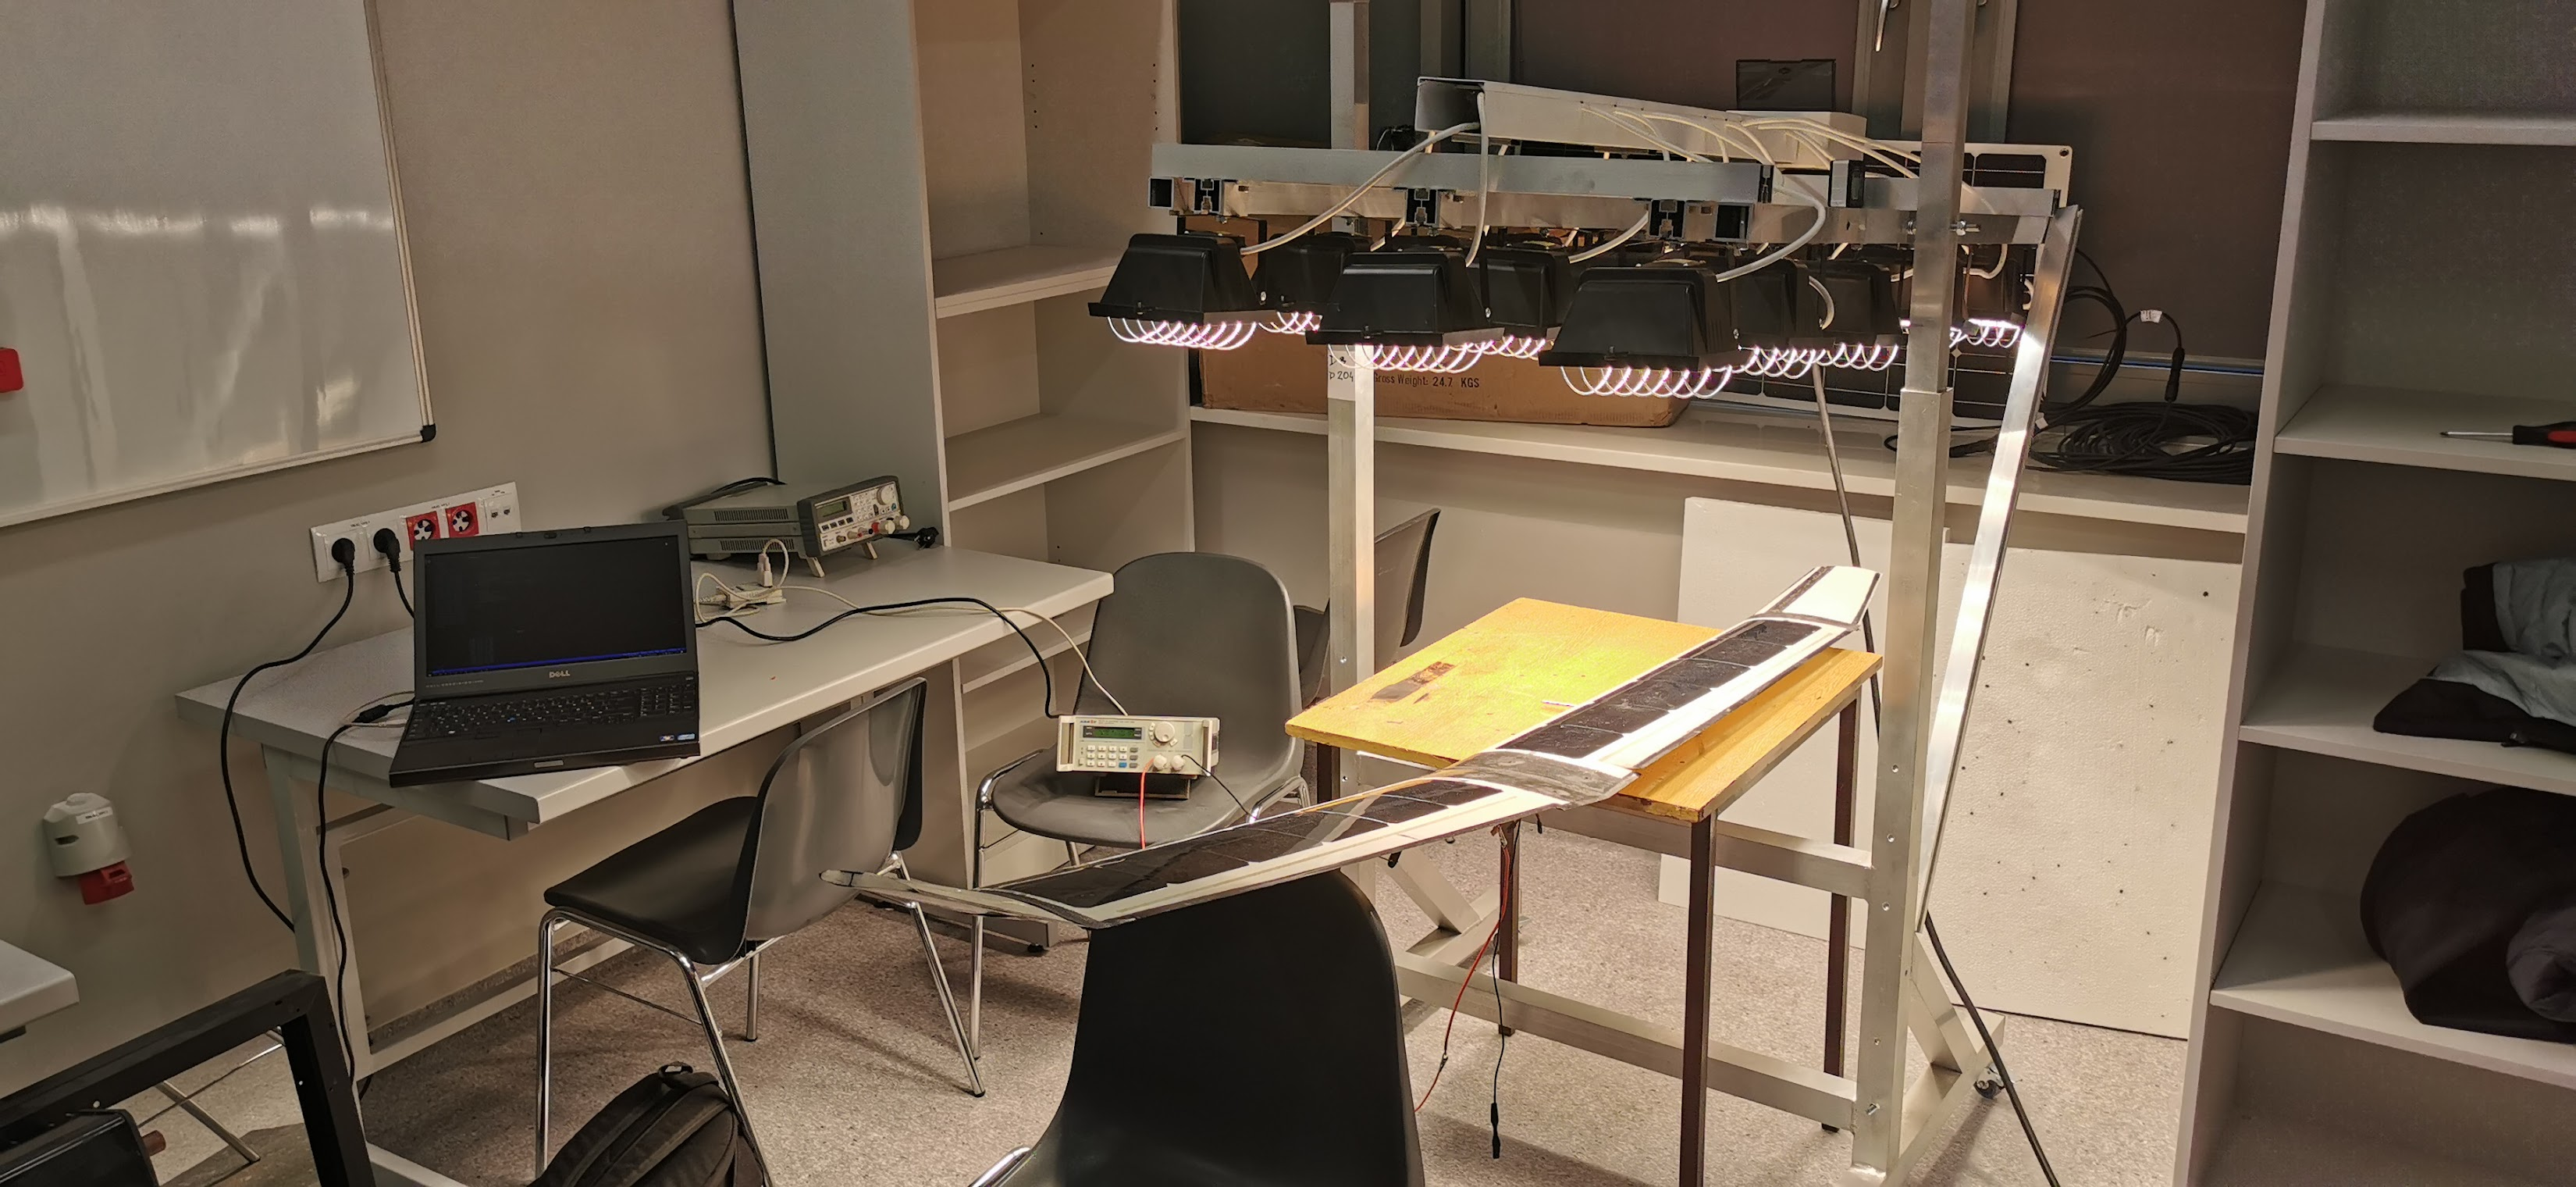
\includegraphics[width=1\textwidth]{badania}
    \caption{Stanowisko pomiarowe do badania ogniw fotowoltaicznych.}
    \label{fig:badanie}
\end{figure}

Dzięki uprzejmości doktora inżyniera Krzysztofa Sornka z Instytutu Zrównoważonego Rozwoju Energetycznego AGH możliwe było przeprowadzenie badań gotowej instalacji na skrzydłach. Z uwagi na brak warunków pogodowych, pomiary zostały przeprowadzone na stanowisku badawczym (zdjęcie \ref{fig:badanie}), które powala na uzyskanie mocy promieniowania świetlnego zbliżonego do warunków podczas słonecznego dnia w lecie na ternie Polski - około 1000$\frac{W}{m^2}$. Warunki takie wytwarza system lamp halogenowych, które niestety bardzo szybko się nagrzewają - pomiary musiały być więc wykonane bardzo sprawnie. Było to możliwe dzięki użyciu skryptu do automatycznego pomiaru przy pomocy modułu sztucznego obciążenia. Badanie trwało więc zaledwie kilkanaście sekund i pozwoliło uniknąć zbytniego przegrzania się ogniw fotowoltaicznych. Instalacja była badana osobno na każdym skrzydle ze względu na ograniczone pole robocze stanowiska. Wynikiem badań było uzyskanie charakterystyk prądowo-napięciowych, a także generowanej mocy w zależności od natężenia wyjściowego. Wyniki zebrano na wykresach \ref{fig:charakterystyki}. Lewe skrzydło było w stanie wytworzyć maksymalnie około 19W energii, prawe - 16 W.

\begin{figure}[ht]
    \centering
    \subfloat{{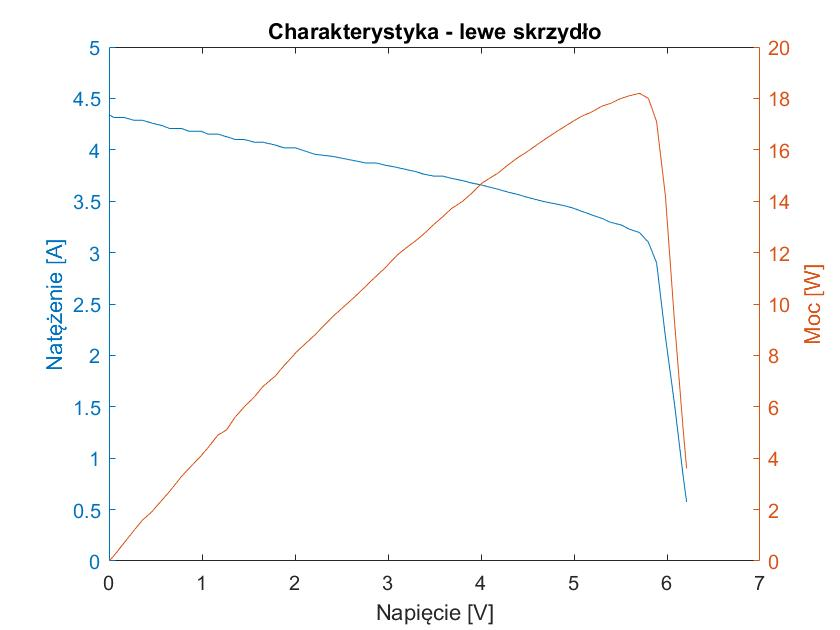
\includegraphics[width=0.45\textwidth]{leweprzetarte} }}
    \qquad
    \subfloat{{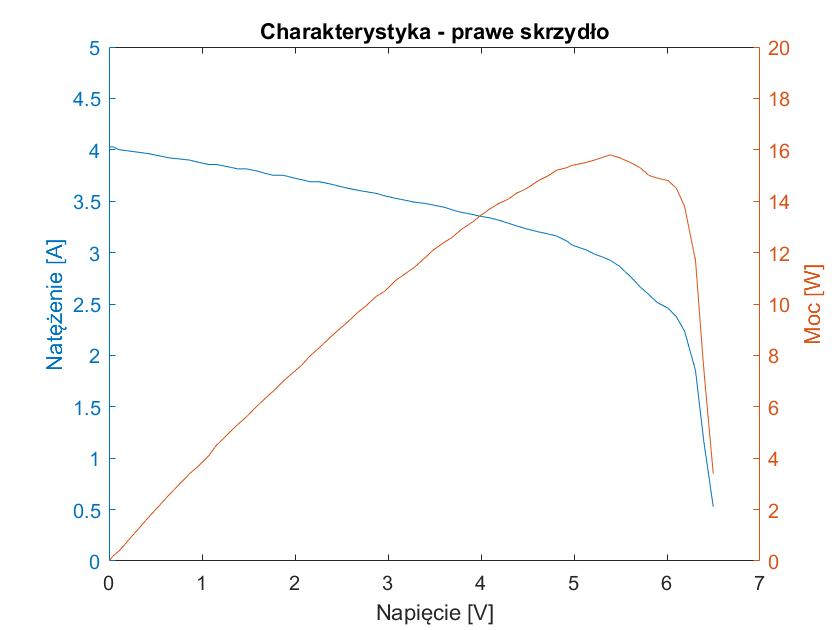
\includegraphics[width=0.45\textwidth]{praweprzetarte} }}
    \caption{Charakterystyka prądowo-napięciowa oraz generowana moc przez instalację na prawym i lewym skrzydle.}
    \label{fig:charakterystyki}
\end{figure}

Na wykresach charakterystyka mocy ma widoczne globalne maksimum, które nazywane jest maksymalnym punktem pracy panelu fotowoltaicznego. Stosowne byłoby zatem użycie modułu MPPT (Maximum Power Point Tracker), który pozwala na dostosowanie zależności napięcia i natężenia w taki sposób, aby zawsze uzyskiwać maksymalną moc. Niestety, takie moduły dostępne na rynku są dostosowane do znacznie większych instalacji, a ich wymiary i waga nie pozwalają na użycie w tak małym samolocie. Prace nad autorskim modułem zajęły by zbyt dużo czasu, dlatego najlepszym rozwiązaniem jest użycie odpowiednio dobranej przetwornicy z rodziny step-up. Przy tak małej instalacji, różnica między użyciem przetwornicy a modułem MPPT jest bardzo mała, ponadto przetwornica pracuje w trybie ciągłym, a moduły MPPT pracują w cyklach ustawiania parametrów co kilka sekund. Zgodnie z założeniem projektowym samolot będzie wykonywał dużą ilość manewrów, zmieniając cały czas kąt nachylenia ogniw względem słońca, zatem przetwornica jest znacznie efektywniejszym rozwiązaniem.

Wybranym modułem został Pololu U3V50AHV, pracujący z natężeniem do 5 A i napięciem 3-30 V. Przetwornicę ustawiono na napięcie wyjściowe 12,6 V, co odpowiada napięciu w pełni naładowanego używanego w samolocie akumulatora Li-Po 3S. Dzięki temu, w przypadku zużycia mniejszej ilości energii przez samolot niż jest w stanie wyprodukować instalacja fotowoltaiczna, jej nadmiar zostanie wykorzystany do ładowania pakietu akumulatora.

Dodatkowym eksperymentem przeprowadzonym podczas badań było sprawdzenie wpływu zabrudzenia instalacji fotowoltaicznej na jej sprawność. Niestety okazało się, że różnica ta nie jest możliwa do wykrycia przy użyciu stanowiska badawczego tego typu - większy wpływ na wyniki miał stopień rozgrzania lamp czy delikatnie inne ustawienie skrzydła na stole roboczym.

\begin{figure}[ht]
    \centering
    \subfloat{{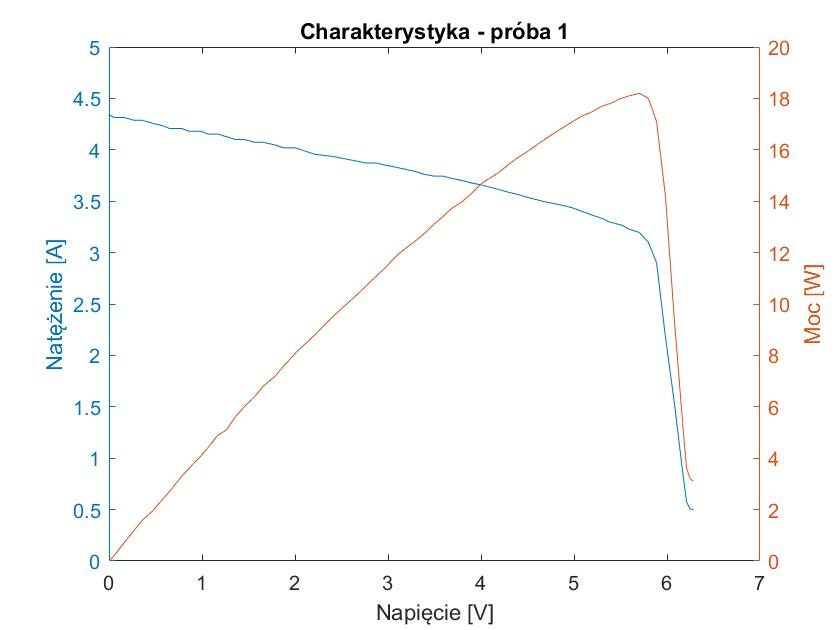
\includegraphics[width=0.45\textwidth]{porownanie1} }}
    \qquad
    \subfloat{{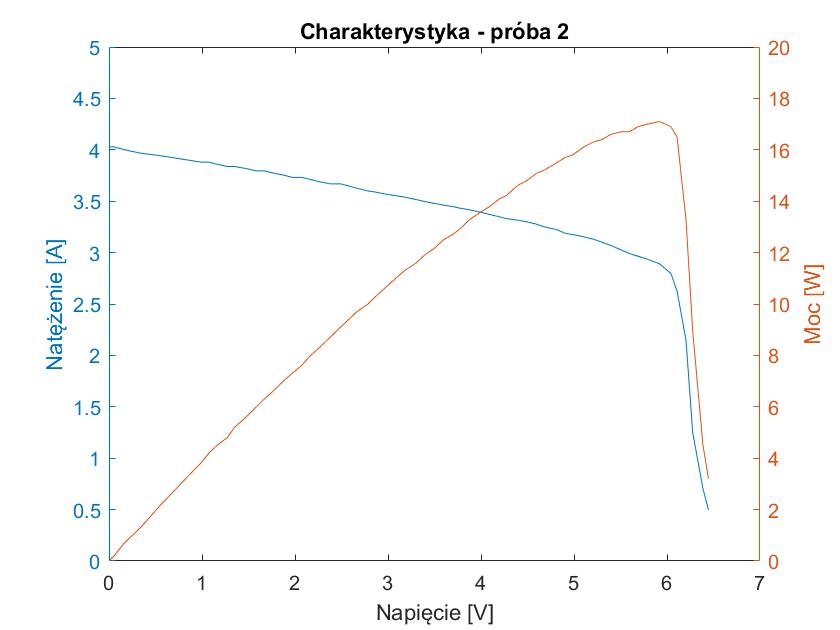
\includegraphics[width=0.45\textwidth]{porownanie2} }}
    \caption{Porównanie charakterystyk prądowo-napięciowych instalacji na lewym skrzydle w odstępie kilkunastu sekund podczas nagrzewania się na stanowisku badawczym.}
    \label{fig:cieple}
\end{figure}

Mimo krótkiego czasu wykonywania pomiarów, halogenowe lampy wytwarzają bardzo dużą ilość ciepła, co przekłada się na spadek sprawności modułów fotowoltaicznych. Widoczne jest to nawet na pomiarach wykonanych w odstępie kilkunastu sekund, gdzie różnica maksymalnej mocy wynosi około 5\%, co przedstawiają wykresy \ref{fig:cieple}. 

Ostatnim wykonanym badaniem była analiza instalacji przy pomocy specjalistycznej kamery termowizyjnej. Podanie napięcia na końce panelu skutkuje stopniowym ogrzewaniem się ogniw. Dzięki tej technice możliwe jest wykrycie uszkodzeń powstałych w procesie laminowania ogniw lub skrzydeł. Miejsca uszkodzone stawiają większy opór elektryczny, a co za tym idzie wytwarzają więcej ciepła przy przepływie energii elektrycznej. W badaniu podano wykorzystano napięcie i natężenie znamionowe ogniw, a różnice w temperaturach sięgały kilku stopni Celsujasza. Na zestawieniu \ref{fig:uszkodzenia} zaobserwować można znacznie większe uszkodzenia szeregu ogniw na prawym skrzydle, co możne tłumaczyć różnicę koło 10\% maksymalnej mocy wytworzonej w poprzednim eksperymencie.

\begin{figure}[ht]
    \centering
    \subfloat{{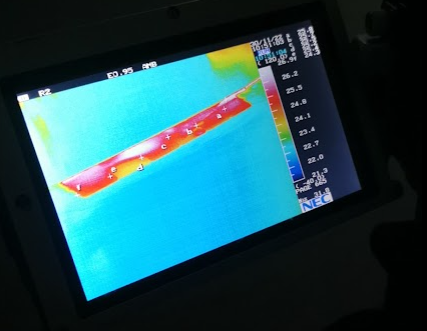
\includegraphics[width=0.45\textwidth]{kamerat} }}
    \qquad
    \subfloat{{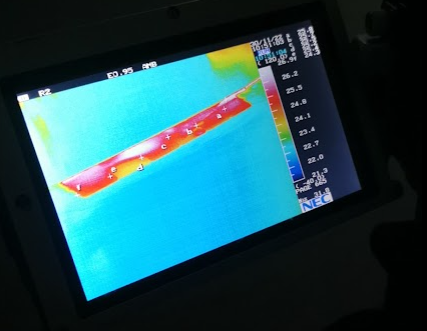
\includegraphics[width=0.45\textwidth]{kamerat} }}
    \caption{Porównanie obserwacji uszkodzeń ogniw fotowoltaicznych na prawym i lewym skrzydle przy pomocy kamery termowizyjnej. [OCZEKIWANIE NA ZDJĘCIA Z KAMERY]}
    \label{fig:uszkodzenia}
\end{figure}

Samolot zdecydowanie najwięcej energii wykorzystuje na podtrzymanie pracy silnika. Na podstawie przeprowadzonych eksperymentów, podczas lotu zużywane jest średnio około 4-6 A. Przekłada się to na zapotrzebowanie energetyczne na poziomie około 50 W. 

Z uwagi na wznios skrzydeł wynoszący 5\textdegree oraz na ciągłą zmianę nachylenia względem słońca, rzeczywista średnia uzyskana moc w powietrzu jest niższa niż podczas statycznego badania. Przeprowadzenie szczegółowych analizy rzeczywistej produkcji energii w trakcie lotu możliwe jest tylko przy odpowiednich warunkach pogodowych mając na uwadze odpowiednie natężenie światła. Na terenie Polski takie warunki osiągnąć można tylko w okresie letnim, jednak na podstawie podobnych eksperymentów prowadzonych w zespole AGH Solar Plane można oszacować średnią rzeczywistą produkcję energii podczas lotu na około 80\% energii produkowanej w stanie spoczynku. Zatem moc znajdującej się na przygotowanym modelu instalacji oszacować można na około 30 W, co stanowi ponad połowę zapotrzebowania energetycznego i przełoży się na znaczne wydłużenie lotu.

Warto zaznaczyć, że uzyskanie instalacji o takiej mocy na skrzydłach samolotu jest bardzo dużym sukcesem i nie było by możliwe bez wielu godzin spędzonych na opracowaniu metod laminowania oraz umieszczania ogniw na skrzydłach przez członków zespołu AGH Solar Plane.

\FloatBarrier
\subsection{Moduł kontrolera lotu}
Pierwszym krokiem podczas pracy nad projektem  było przygotowanie listy parametrów, które są brane pod uwagę przez pilota podczas zdalnego terowania modelem. Są to: wysokość, orientacja, prędkość względem ziemi, prędkość względem wiatru, położenie samolotu oraz dalsza planowana trasa. Wszystkie te wymienione elementy muszą w analogiczny sposób być brane pod uwagę przez autonomiczną jednostkę sterującą, a zbierane muszą być przy pomocy sensorów i czujników umieszczonych na pokładzie samolotu. 

Jednym z kluczowych założeń kontrolera lotu jest jego nieprzerwane, niezatrzymane i nieopóźnione działanie w podczas pracy. Utrata kontroli nad samolotem oznacza niemal pewne uderzenie w ziemię w ciągu zaledwie kilku sekund. Dlatego jako główny komputer pokładowy został wybrany mikrokontroler Teensy 4.0. Dysponuje on mikroprocesorem ARM Cortex-M7, taktowanym w trybie standardowym z częstotliwością 600 MHz. Jego innymi istotnymi zaletami są możliwość generowania sygnału PWM przez większość wyjść cyfrowych, duża pojemność pamięci Flash (1984K) oraz RAM (1024 KB), 7 portów szeregowych UART, a także możliwość programowania w środowisku Arduino IDE (z rozszerzeniem Teensyduino). Ta ostatnia cecha jest o tyle ważna, że pozwala na użycie bibliotek do sensorów, które są najczęściej przygotowane właśnie pod to środowisko. Ich migracja na inne technologie mogła by być problematyczna. 

Warto zauważyć, że teoretycznie jeszcze lepszymi parametrami cechują się moduły komputerów jednopłytkowych (ang. single-board computer), jak na przykład Raspberry Pi Zero W, na którym można uruchomić system Raspbian z rodziny UNIX. Uruchomienie programu kontrolera na takim mikrokomputerze byłoby prawdopodobnie stabilniejsze od strony oprogramowania i pozwalało na łatwiejsze zarządzanie wyjątkami i błędami, jednakże w przypadku zawieszenia się systemu operacyjnego lub jakiegokolwiek innego czynnika mogącego przerwać płynność działania programu, bardzo prawdopodobne jest utracenie kontroli nad samolotem. Dodatkowo, system operacyjny uruchamia się w najlepszym czasie około kilkunastu sekund, co w przypadku nieplanowanego restartu urządzenia w powietrzu, wywołanego na przykład chwilowym spadkiem napięcia na przetwornicy, oznacza pewne rozbicie modelu. Teensy uruchamia się w czasie bliskim sekundy, dodatkowo przed inicjalizacją czujników (mogącą trwać 2-3 sekundy) program sprawdza w pamięci EEPROM, czy samolot nie został uprzednio uzbrojony. Jeżeli tak, czujniki pozostają wyłączone, natomiast samolot przechodzi w awaryjny tryb manualny. To rozwiązanie zapewnia najwyższe bezpieczeństwo.

Pierwszy prototyp autorskiego kontrolera lotu wykorzystywał następujące moduły:
\begin{enumerate}
\item Mikrokontroler Teensy 3.2
\item Czujnik AltIMU v10
\item Odbiornik Spectrum DSMX DX6
\item Moduł GPS SparkFun NEO-M9N
\item Moduł karty microSD
\end{enumerate}

Całość umieszczona była we fragmencie pianki ochronnej i miała posłużyć do pierwszego sprawdzenia działania systemu. Mikrokontroler miał za zadanie gromadzić dane z czujników oraz odbierać sygnał od aparatury sterującej i przekazywać go na wyjście. W skład elektroniki pokładowej wchodziły też cztery serwomechanizmy sterujące powierzchnymi sterowymi (lotki, stery kierunki i wysokości), bezszczotkowy silnik, regulator prędkości (ESC) oraz pakiet baterii Li-Po 3S 2600mAh, który pozwalał na kilkanaście minut lotu. W module ESC znajduje się przetwornica typu UBEC 5V, która służyła jako źródło zasilania układu.
 
Wraz z kolejnymi etapami prac moduł karty microSD został zastąpiony przez moduł radiowy HC-12 operujący na częstotliwości 433 MHz. Wysyłanie danych w czasie rzeczywistym oraz ich zapis po stronie stacji odbiorczej okazał się bardziej praktycznym rozwiązaniem. Czujnik AltIMU v10, w skład którego wchodzi żyroskop, akcelerometr, magnetometr oraz wysokościomierz ciśnieniowy, okazał się działać nieprawidłowo. Został wymieniony na znacznie precyzyjniejszy moduł SparkFun ICM 20948. Dzięki wbudowanemu w bibliotekę algorytmowi DMP (InvenSense Digital Motion Processor) jest on w stanie z niesamowitą precyzją podać kąty Eulera rotacji (roll, pitch, yaw) oraz dokonywać autokalibracji podczas działania. Ma on niestety również wady: potrzebuje stosunkowo dużej ilości mocy obliczeniowej do działania oraz wysokiego taktowania procesora (producent zaleca co najmniej 100 MHz), jego poprawne działanie wymaga znacznie trudniejszej implementacji od strony oprogramowania, a także nie jest w stanie wskazać bezwzględnego położenia w osi yaw, zatem przed każdym startem należy skalibrować go ręcznie. Czujnik orientacji jest jednym z ważniejszych elementów kontrolera lotu i bardzo kluczowa jest jego powtarzalność i precyzja działania - wybrany moduł firmy SparkFun spełnia wyznaczone kryteria, a brakujący czujnik wysokości został zastąpiony zewnętrznym modułem LPS25HB. Teensy 3.2 zostało zastąpione przez Teensy 4.0 z powodu lepszych parametrów oraz kompatybilności sprzętowej z biblioteką TensorFlowLite.

Po ostatecznym wyborze modułów przygotowana została druga wersja urządzenia, wraz  z testową płytką PCB. Jej projekt wykonany został w programie KiCAD (rysunek \ref{fig:stara}), i miał zapewnić stabilną pracę urządzenia oraz wymiary umożliwiające wkładanie go do samolotu testowego EasyGlider 4. 

\begin{figure}[ht]
    \centering
    \subfloat{{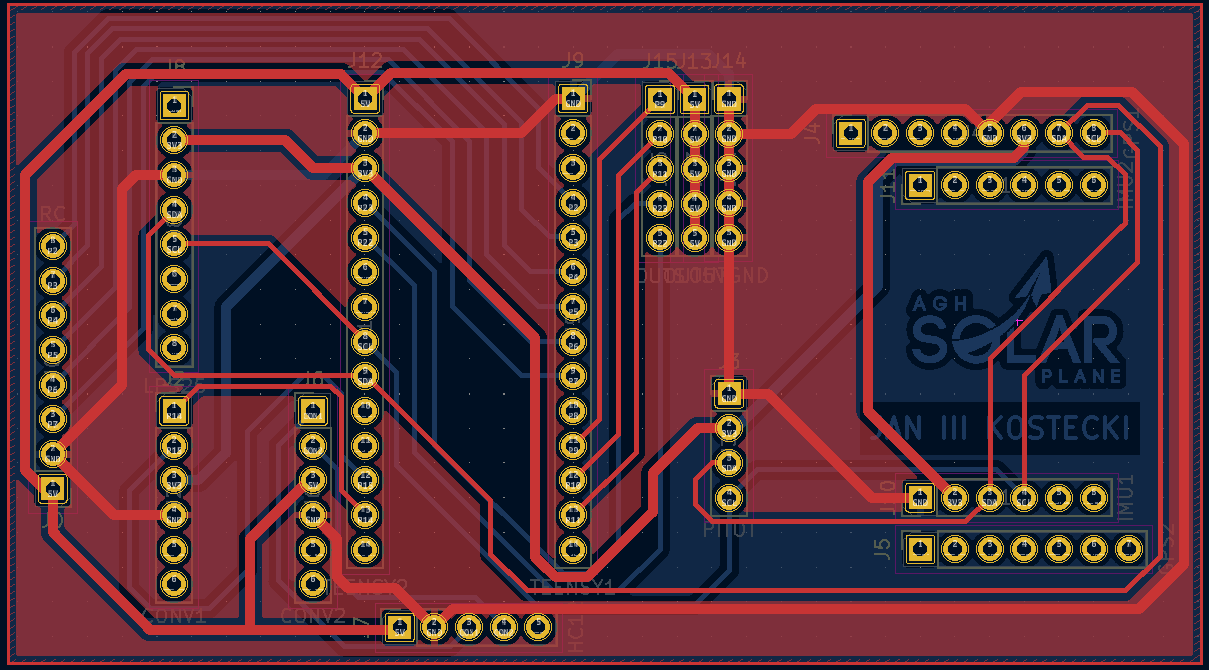
\includegraphics[width=0.45\textwidth]{plytkastara} }}
    \qquad
    \subfloat{{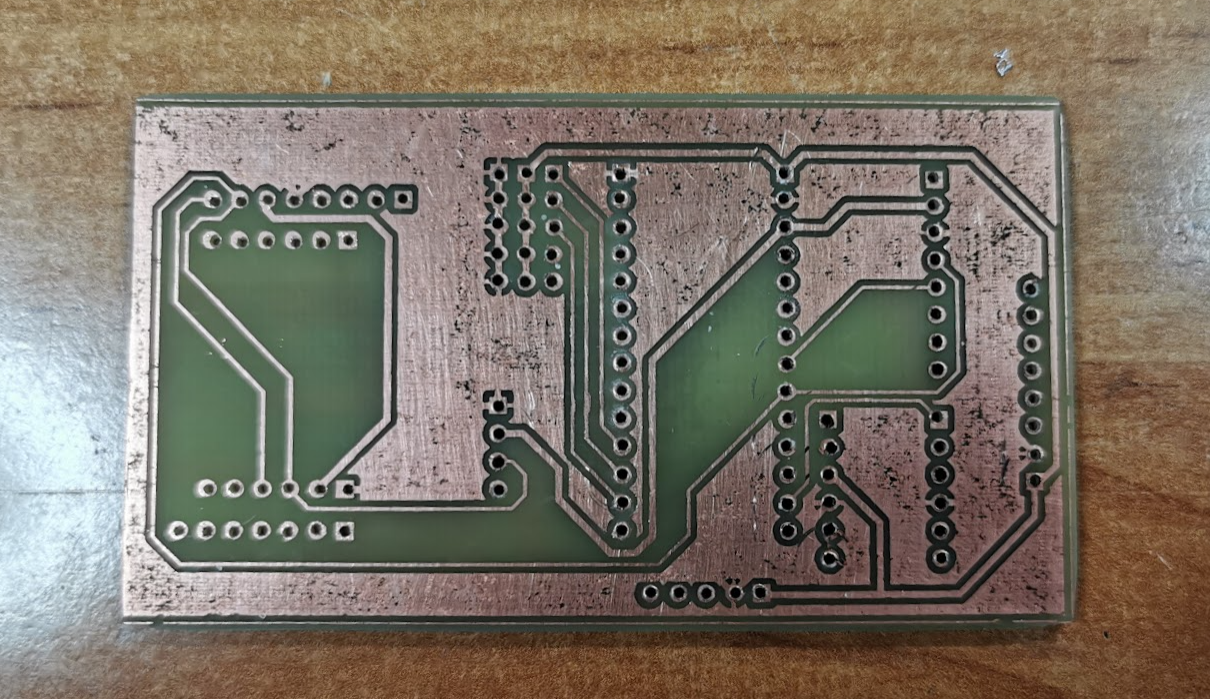
\includegraphics[width=0.45\textwidth]{pcb} }}
    \caption{Projekt w programie KiCAD oraz wykonana płytka metodą termotransferu.}
    \label{fig:stara}
\end{figure}

Przygotowany projekt jest dwustronną płytką PCB o wymiarach 90 na 50 mm. Wykonana ona została przy pomocy metody termotransferu tonera na specjalny laminat o grubości 1.5 mm. Następnie niepotrzebna miedź została rozpuszczona w roztworze Nadsiarczanu Sodu. Efekt jest widoczny na zdjęciu \ref{fig:stara}

Aby zapewnić możliwość wymiany elementów, do gotowej płytki przylutowo żeńskie gniazda typu goldpin raster 2.54 mm, które są kompatybilne ze wszystkimi wykorzystanymi modułami i pozwalają na szybkie przyłączanie oraz odłączanie. Gotowy kontroler przedstawiony został na zdjęciu \ref{fig:starycaly}. Część elektroniki jest na zdjęciu niewidoczna, znajduje się po drugiej stronie płytki.

\begin{figure}[ht]
    \centering
    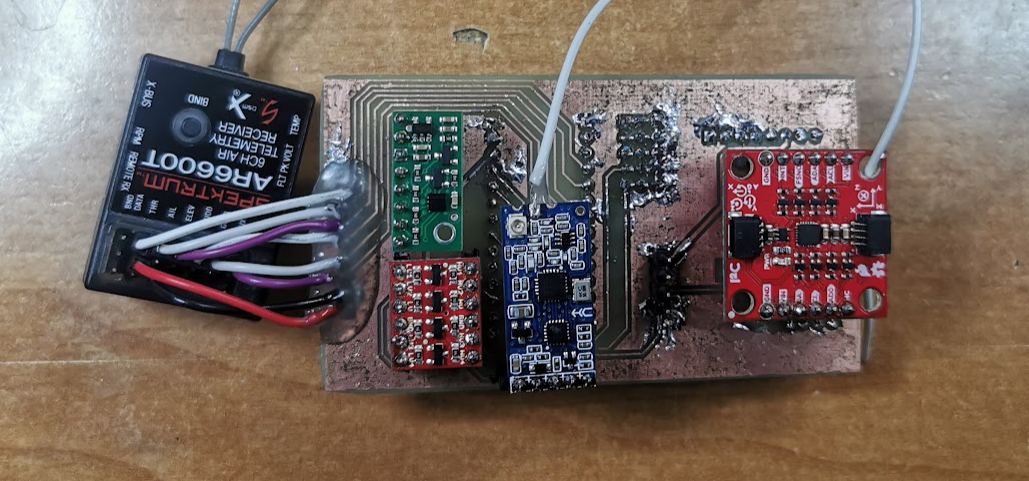
\includegraphics[width=1\textwidth]{kontorolerstary}
    \caption{Gotowy kontroler lotu na autorskiej płytce PCB.}
    \label{fig:starycaly}
\end{figure}

Po pierwszych próbach kontrolera w trakcie lotu okazało się, że czujnik wysokości zwraca bardzo niedokładne wyniki. Analiza zebranych danych wykazała, że sam czujnik działa poprawnie, jednak przez ruch silnika i śmigieł oraz pęd powietrza przelatującego przez kadłub samolotu, wyniki w żaden sposób nie pokrywają z faktycznym stanem rzeczy. Widoczne jest to na wykresie porównującym wyniki z czujnika ciśnieniowego oraz modułu GPS (rysunek \ref{fig:alti}) - według pierwszego z nich samolot ląduje 230 metrów ponad miejscem startu. Dużo bardziej precyzyjny okazał się pomiar wysokości przy pomocy modułu GPS i na jego podstawie opierane były dalsze obliczenia.

\begin{figure}[ht]
    \centering
    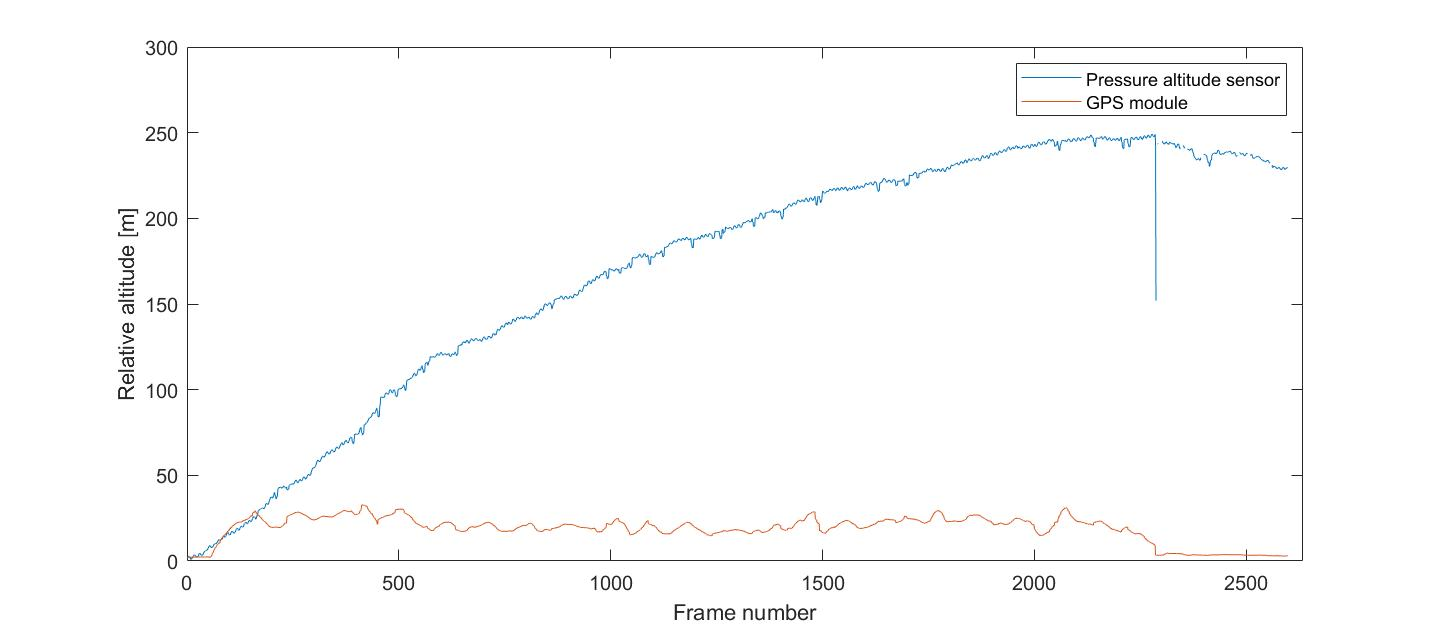
\includegraphics[width=1\textwidth]{alti}
    \caption{Porównanie odczytów wysokości z czujnika LPS25HB oraz modułu GPS.}
    \label{fig:alti}
\end{figure}

   \begin{figure}[ht]
    \centering
    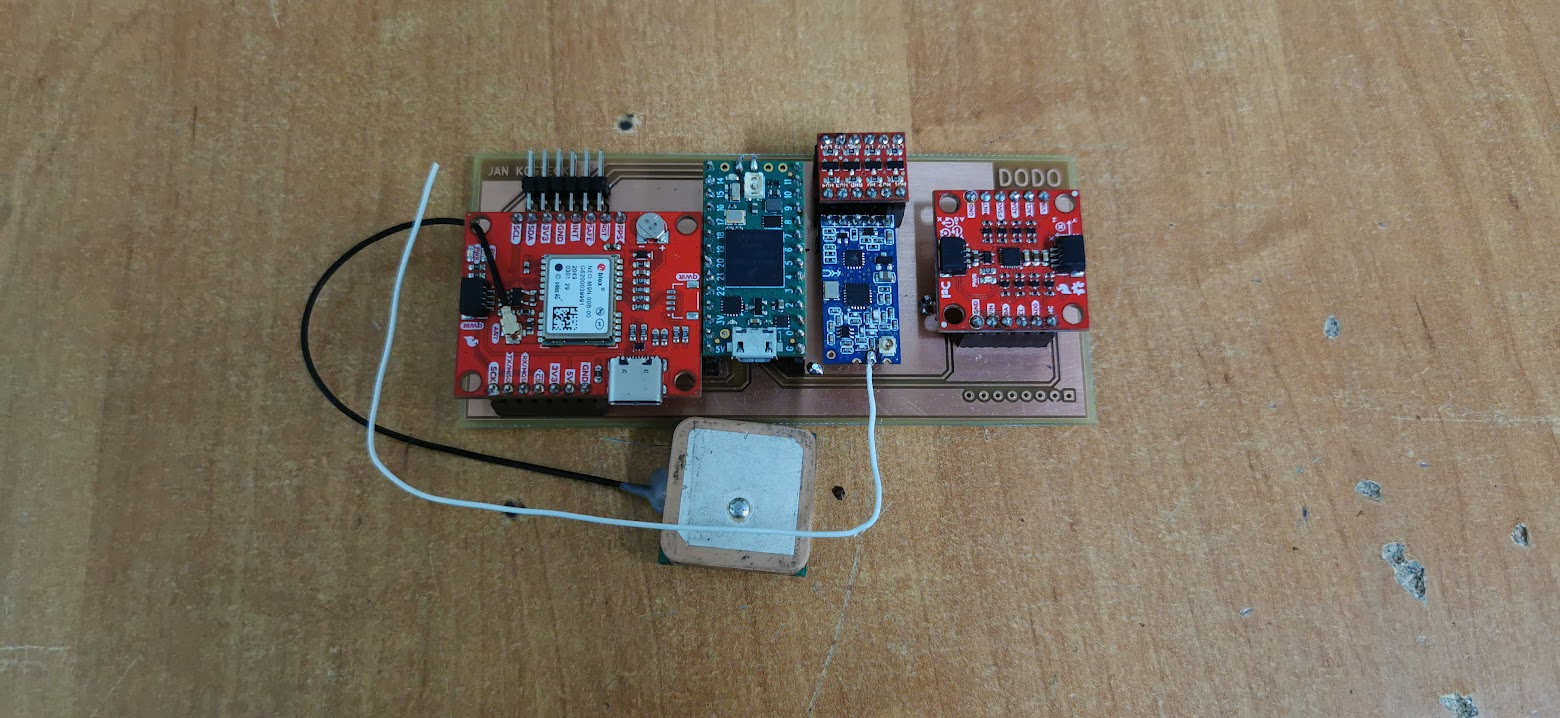
\includegraphics[width=1\textwidth]{dodokontroler}
    \caption{Finalny moduł kontrolera lotu.}
    \label{fig:dodokontroler}
\end{figure}

Warto zaznaczyć, że widoczna na zdjęciu \ref{fig:starycaly} płytka miała charakter prototypowy, stąd widoczne niedoskonałości wykonania oraz ślady wprowadzanych poprawek. Po ustaleniu ostatecznej listy komponentów oraz skonstruowaniu dedykowanego samolotu, zaprojektowana została ostateczna wersja modułu kontrolera. Na płytce PCB wszystkie moduły zostały umieszczone po jednej stronie, zmieniony został także sposób podłączenia do układu w samolocie – ręczne wpinanie kabli do serw, ESC oraz rurki Pitota zostało zastąpione jednym gniazdem (zdjęcie \ref{fig:gniazdo}), które przy okazji pełni rolę mocowania. Dzięki temu proces umieszczenia i wyjęcia kontrolera z samolotu trwa dosłownie sekundę i nie naraża elementów na uszkodzenie. Z uwagi na ograniczenia czasowe projektu otwory w płytce PCB nie zostały poddane procesowi metalizacji, sygnał przekazywany jest między warstwami za pomocą przelotek. Zrezygnowano także z umieszczenia na płytce ciśnieniowego czujnika wysokości. Gotowy moduł widoczny jest na zdjęciu \ref{fig:dodokontroler}.

   \begin{figure}[ht]
    \centering
    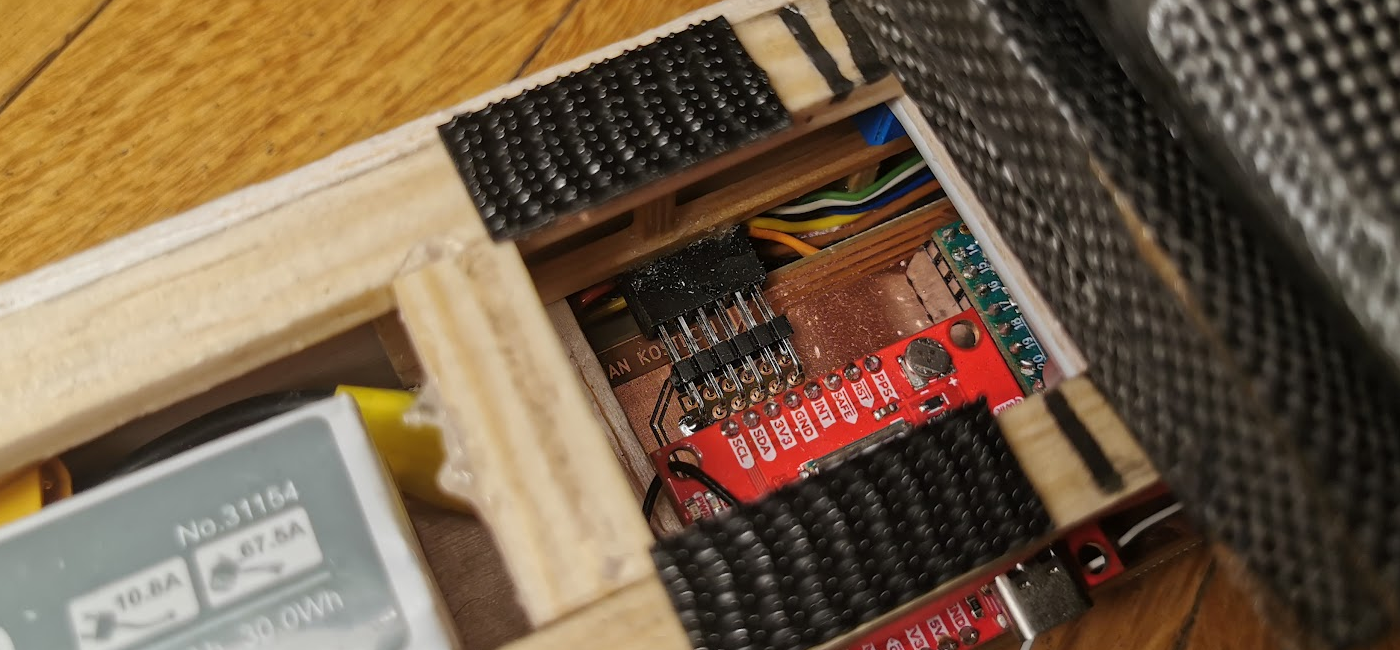
\includegraphics[width=1\textwidth]{gniazdo}
    \caption{Gniazdo mocujące, sygnałowe i zasilające kontrolera lotu.}
    \label{fig:gniazdo}
\end{figure}


W skład elektorniki podkładowej samolotu wchodzą także serwomechanizmy do poruszania powierzchniami sterowymi samolotu. Z uwagi na ich rozmiar, wybrane zostały serwomechanizmy GO-17 MG firmy Pelikan. Posiadają one moment obrotowy od 2,2 $\frac{kg}{cm}$ przy napięciu zasilającym 4,8V do nawet 2,5 $\frac{kg}{cm}$ przy napięciu 6 V (w samolocie napięcie zasilające za przetwornicą wynosi znamionowo 5V, w praktyce ta wartość waha się w zakresie 5 V-5.5 V). Silnik napędzający samolot umieszczony jest w przedniej części kadłuba, razem z elektronicznym regulatorem prędkości ESC. Wybranym modelem został Dualsky Ecko V2 2814 970 kV. Jego chwilowa moc maksymalna wynosi nawet do 400W, przy obciążeniu prądowym 33A. Zgodnie z zaleceniem producenta, dobrane do niego zostały śmigła 11x7.  

 \clearpage
\subsection{Oprogramowanie kontrolera lotu}
Ciągłość pracy kontrolera jest jednym z najważniejszych założeń projektowych – jak już zostało podkreślone, jakikolwiek przestój w pracy może się wiązać z rozbiciem samolotu. Całe oprogramowanie znajduje się na mikrokontrolerze Teensy 4.0. Po uruchomieniu, pierwszymi czynnościami są inicjalizacje:
\begin{enumerate}

\item Portów szeregowych do komunikacji
\item Serwomechanizmów 
\item Biblioteki odczytującej dane z odbiornika
\item Odczytanie wartości stanu uzbrojenia silnika z pamięci EEPROM

\end{enumerate}

Jeżeli silnik został uzbrojony (włączony z poziomu oprogramowania) oznacza to, że samolot najprawdopodobniej znajduje się w powietrzu, dlatego od razu uruchamiany jest tryb awaryjny, aby pilot miał największe szanse na uratowanie modelu. W innym przypadku inicjalizowane są czujniki IMU oraz GPS.

Oprogramowanie ma pozwolić na dwa tryby lotu – manualny oraz autonomiczny. W pierwszym z nich dane z czujników nie mają wpływu na lot, sygnał z aparatury jest przekazywany bezpośrednio na wyjścia.
 
\begin{figure}[ht]
    \centering
    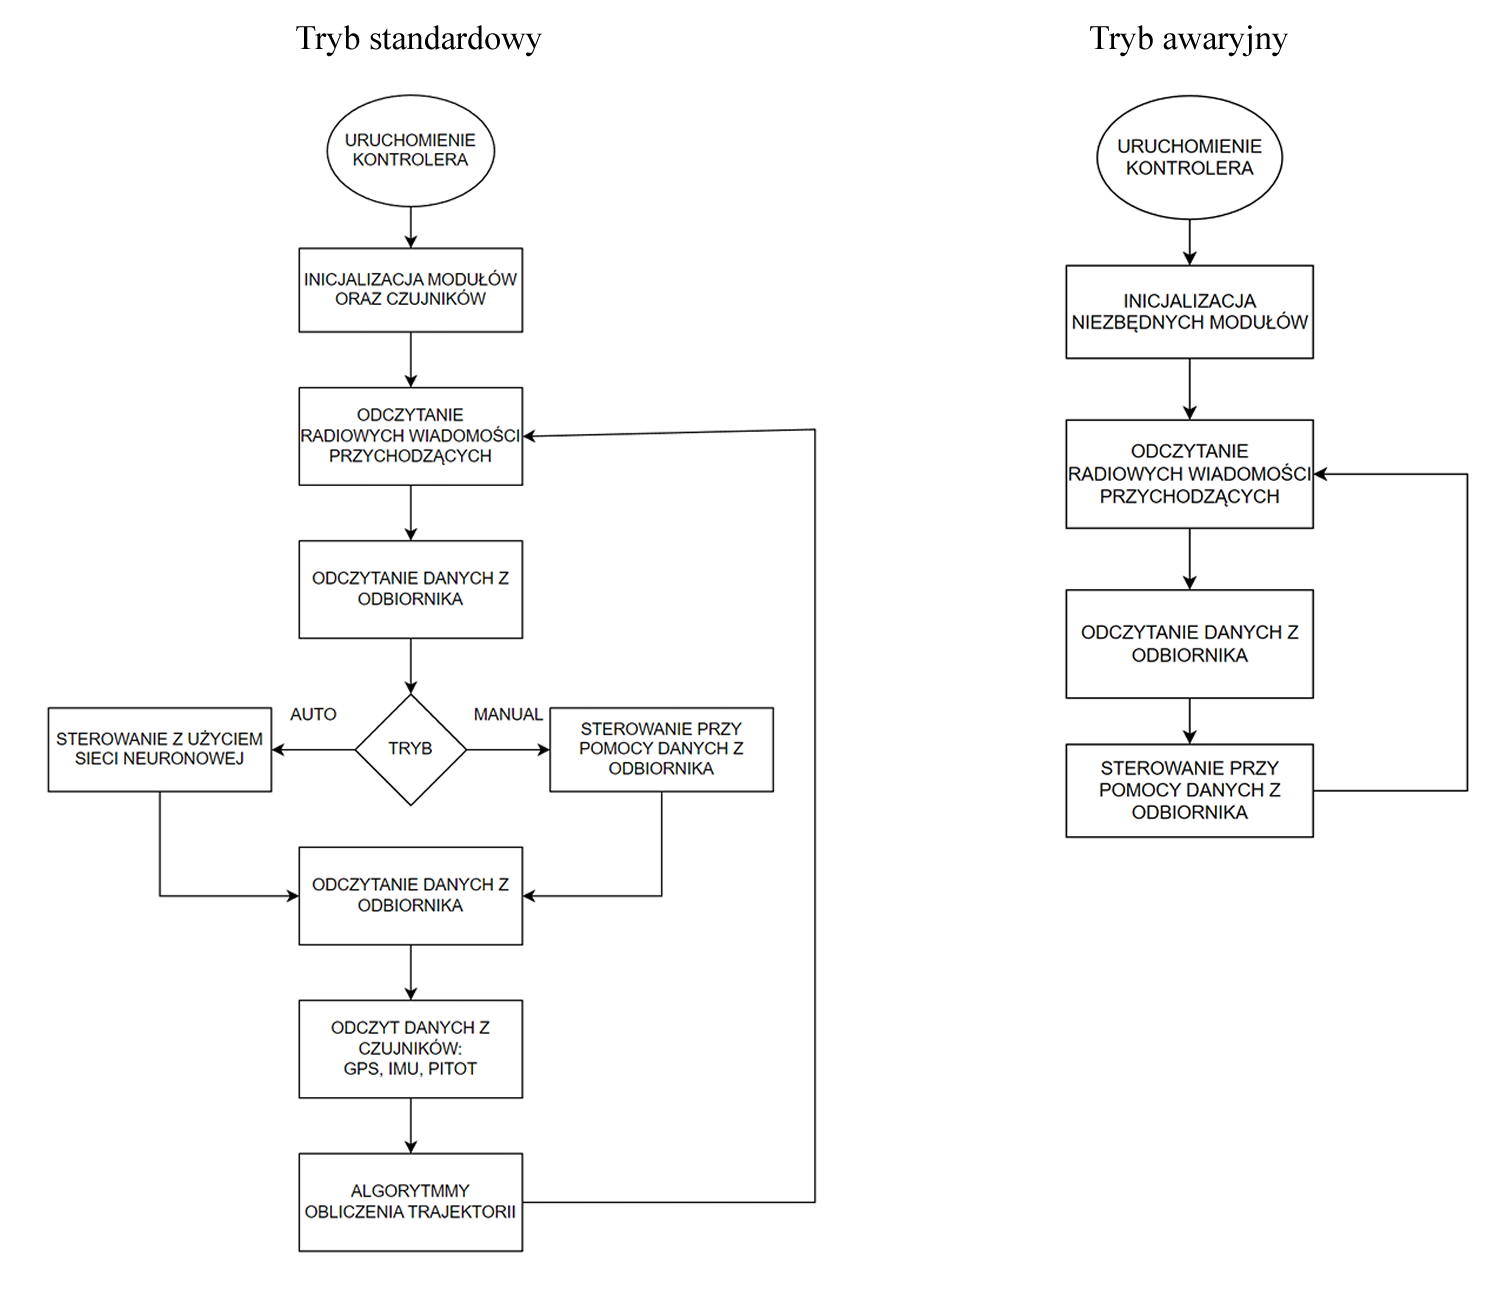
\includegraphics[width=1\textwidth]{diagramy}
    \caption{Schematy blokowe działania oprogramowania w trybie standardowym i awaryjnym.}
\end{figure}

Poszczególne elementy programu działają z różna częstotliwością - zostały one zebrane w Tabeli \ref{table:hz}.


\begin{table}[H]
\centering
\begin{tabular}{| l | l |}
\hline
Element programu & Częstotliwość działania \\
\hline
Odczyt danych z odbiornika & 50 Hz \\
Sterowanie – tryb manualny & 50 Hz \\
Sterowanie – tryb autonomiczny & 20 Hz \\
Odczyt danych z sensora IMU & $\sim$100 Hz \\
Odczyt danych z rurki Pitota & 20 Hz \\
Odczyt danych z modułu GPS & 10 Hz \\
Odczyt wiadomości radiowych & $\sim$1000 Hz \\
\hline

\end{tabular}
\caption{Zestawienie częstotliwości działania elementów programu.}
\label{table:hz}
\end{table}

Warto zauważyć, że odbiór danych z czujnika IMU odbywa się z prędkością około 100 MHz - wynika to z faktu, że algorytm DMP powinien pobrać zakolejkowane w buforze dane najszybciej, jak to możliwe, co znacznie zwiększa precyzję działania sensora. W każdej pętli wysyłane do modułu jest zapytanie, czy nowe dane są dostępne i jeżeli tak, są one pobierane. Użyty moduł GPS jest w stanie określać lokalizację z częstotliwością do 25 Hz, jednak przy prędkości przelotowej samolotu, pozycja generowana częściej niż 10 razy na sekundę mieści się w zakresie niedokładności pomiarowej modułu. Odczyt wiadomości radiowych działa z tak wysoką częstotliwością, ponieważ odbywa się w każdej iteracji głównej pętli programu, której średni czas wykonania jest nieco niższy niż 1ms (zależy od ilości wykonanych operacji).

Dane z rurki Pitota pełniącej funkcję czujnika prędkości wiatru względem samolotu, nie są w żaden sposób filtrowane po stronie sensora, dlatego na wyniki zostaje nałożony algorytm średniej kroczącej kilku ostatnich rezultatów.

Niestety wykorzystanie zewnętrznych bibliotek do czujników, dostępnych w oficjalnych źródłach producenta, nie pozwala na pełne zarządzanie czasem pracy i oczekiwania procesora. Najbardziej newralgicznym punktem, mogącym zaburzyć działanie pracy kontrolera, jest oczekiwanie na dane przychodzące na magistrali $I^2C$ - w przypadku błędu po stronie sensora lub innego przerwania połączenia, czas ten może wynosić nawet kilkadziesiąt milisekund, co przekłada się na całkowitą utratę kontroli nad samolotem. Dlatego wprowadzone zostało dodatkowe zabezpieczenie - po wykryciu takiego błędu kontroler wchodzi w tryb awaryjny, który pozwala tylko i wyłącznie na sterowanie samolotem w trybie manualnym oraz odbieranie komend ze stacji bazowej. Wszystkie czujniki pozostają wyłączone do czasu rozbrojenia silnika i restartu urządzenia.

W pamięci EEPROM mikrokontrolera zapisywane są dane dotyczące kalibracji lokalnego  układu współrzędnych, dzięki czemu nie trzeba ich wysyłać za każdym razem po uruchomieniu systemu. Są to pozycje dwóch kolumn, skala w dwóch osiach oraz kąt zawarty między równoleżnikiem a półprostą zaczynającą się w lewej kolumnie i przechodzącej przez prawą. W pamięci zapisana jest też informacja o uzbrojeniu silnika oraz lokalizacje kolejnych waypointów. Sumarycznie wykorzystane są 142 bajty pamięci. Planowane było wykorzystanie zewnętrznej pamięci EEPROM lub tej wbudowanej w mikrokontroler do aktualizowania algorytmu sieci neuronowej bez konieczności podłączania kabla, jednak takie rozwiązanie okazało się być niepraktyczne ze względu na ilość wysyłanych danych i konieczność sprawdzenia ich poprawności. Dodatkowo ponowne inicjalizowanie sieci stworzonej przy użyciu gotowych bibliotek mogło się okazać niemożliwe. Przyjętym rozwiązaniem został ulepszony dostęp do portu microUSB mikrokontorlera, co pozwala na aktualizację oprogramowania w zaledwie kilka sekund, a sieć zapisana jest w pamięci Flash.

\FloatBarrier
\paragraph{Algorytm estymacji trajektorii}\mbox{}

Jednym z najważniejszych aspektów wykonania precyzyjnego manewru samolotem jest wzięcie pod uwagę kilku kolejnych punktów na planowej trasie, ze względu na charakter sterowania tego typu statkiem powietrznym. Aby umożliwić jak najkrótszy czas przygotowania samolotu do lotu, jego trasa określana jest przy pomocy pozycji dwóch kolumn, wokół których automatycznie ustalane są waypointy. Obliczenia pozycji punktów na mapie prowadzone są po stronie aplikacji webowej, a następnie wysyłane na samolot. Dla ułatwienia obliczeń i wizualizacji, po skalibrowaniu terenu, samolot korzysta z lokalnego układu współrzędnych, do którego transformowane są koordynaty GPS. Powierzchnia, po której porusza się samolot jest na tyle mała w skali krzywizny planety, że przyjąć można lokalny układ współrzędnych jako dwuwymiarowy układ kartezjański. 

\textbf{Uwaga:} zgodnie z założeniem projektowym obszar lotu oraz odległość między kolumnami są stałe.

 \begin{figure}[ht]
    \centering
    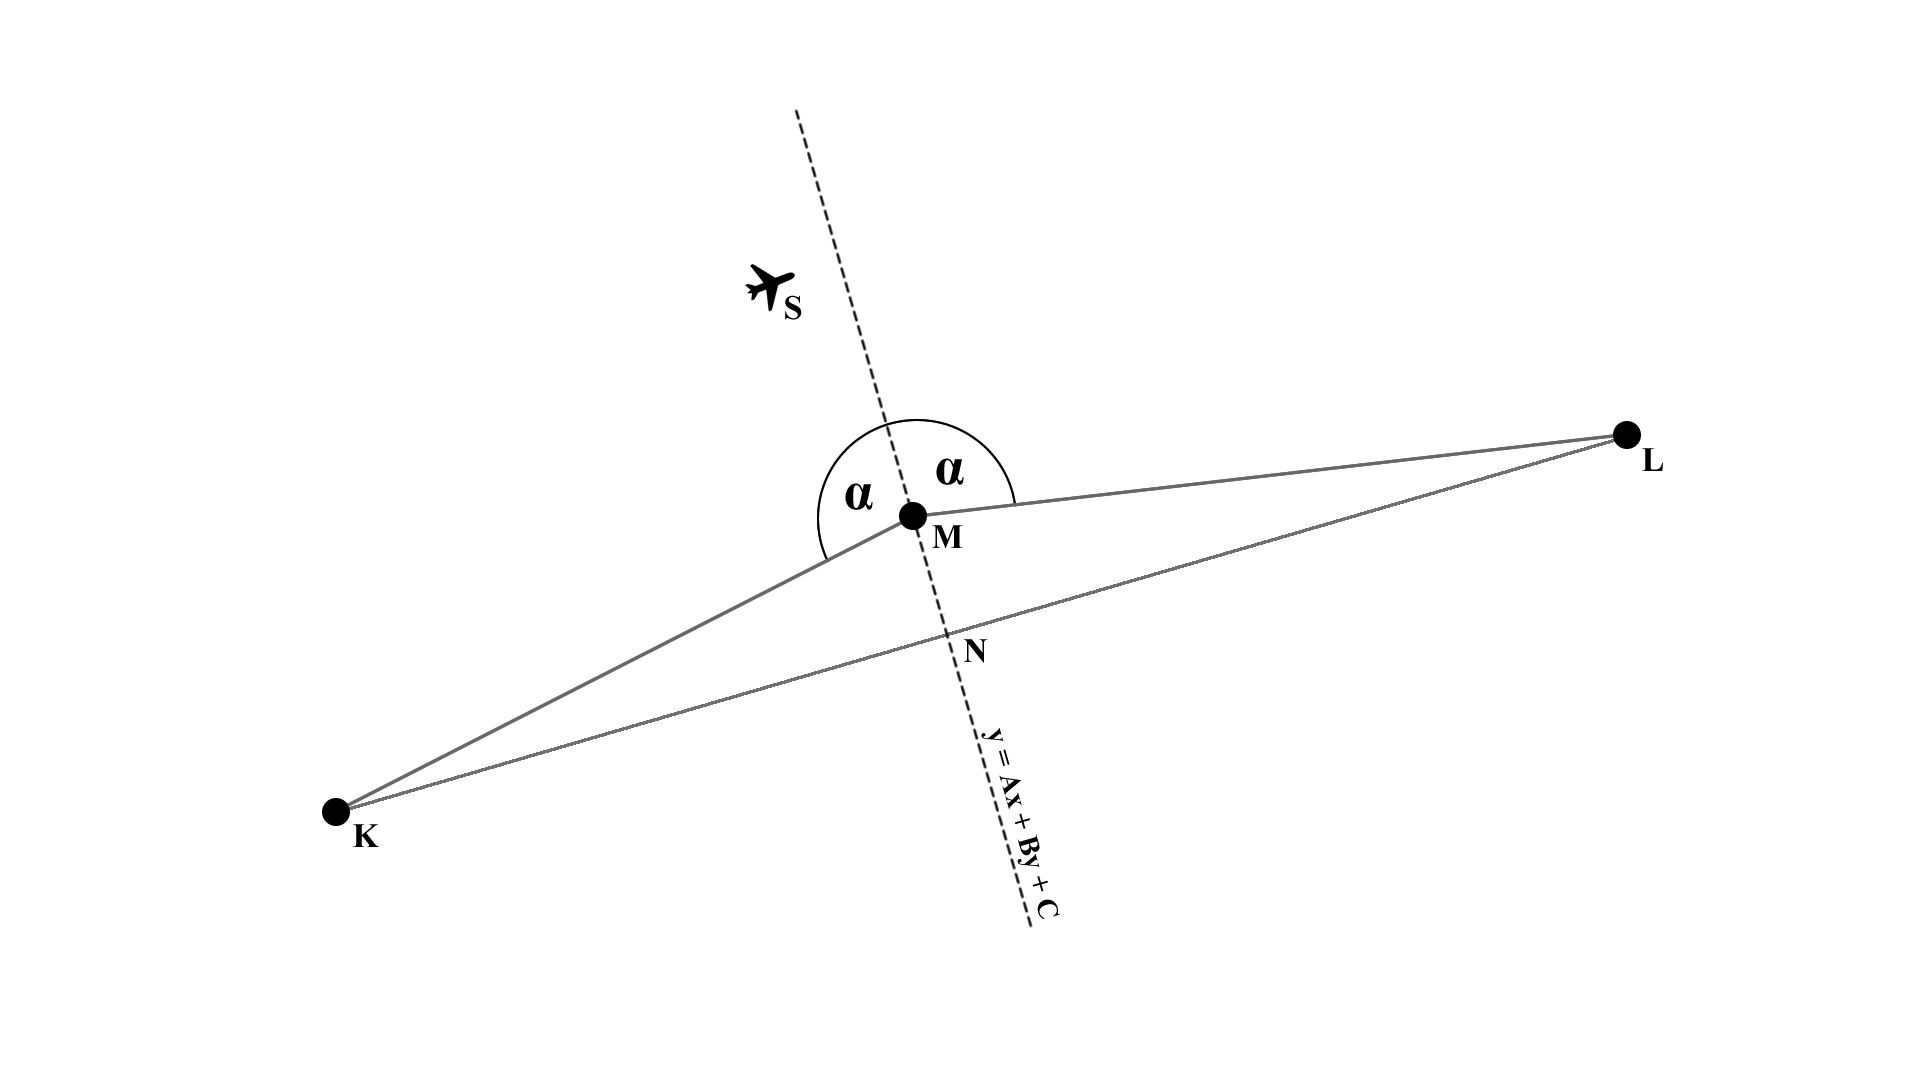
\includegraphics[width=1\textwidth]{nextwaypoint}
    \caption{Schemat położenia samolotu pomiędzy waypointami i linia zaliczenia punktu.}
    \label{fig:wp}
\end{figure}

Aby wyznaczyć trajektorię lotu, należy najpierw określić, między którymi waypointami znajduje się samolot. Na początku działania programu zakładamy, że znajduje się on przed pierwszym, centralnym punktem, po czym sprawdzamy następujący warunek: wyznaczana jest prosta przechodząca przez kolejny punkt na trasie tak, aby kąty zawarte między nią a prostymi przechodzącymi przez ten punkt i z nim sąsiadującymi były równe, jak pokazano na schemacie \ref{fig:wp}. Jeżeli pozycja samolotu wprowadzona do równania takiej prostej będzie mieć przeciwny znak, niż po wprowadzeniu pozycji poprzedniego punktu, można uznać punkt za zaliczony. 


\begin{gather*}
	\text{Szukana prosta jest opisana równaniem:} \\ 
	y = Ax + By + C \\ 
	\text{Korzystając z twierdzenia o dwusieczej kąta w trójkącie:} \\	
	\frac{|KM|}{|LM|} = \frac{|KN|}{|LN|} \\
	=>|KN| = \frac{|KL|}{1+\frac{|KM|}{|KM|}} \\
	\vec{KN} = [L_x - K_x, L_y - K_y] \frac{|KN|}{|KL|} \\
	\text{Zatem:} \\
	A = -\frac{M_y - N_y}{M_x - N_x} \\
	B = 1 \\
	C = -N_y - A \cdot N_x \\
	y(x, y) = Ax + By + C  \\
	\text{Linia zmiany puntu zostaje przekroczona, jeśli:} \\
	H(y(S_x, S_y)) \neq  H(y(K_x, K_y)) \\
	\text{Gdzie:} \\
	H(x) = \begin{cases} 1, & x >= 0 \\ -1, & x < 0 \end{cases}	 
\end{gather*}

Kąty na trasie obliczane są według poniższej zależności, zgodnie ze wzorem na wartość kąta zawartego pomiędzy dwoma wektorami:

\begin{gather*} 
	\text{Przyjmujemy A, B, C jako kolejne punkty} \\ 
 	\vec{a} = [A_x - B_x, A_y - B_y] \\
 	\vec{b} = [C_x - B_x, C_y - B_y] \\
 	angle = 	\arccos{\frac{\vec{a} \cdot \vec{b}}{|\vec{a}||\vec{b}|} } \cdot H(a_x b_y -  a_y b_x) \\ 
 	Gdzie:
 	H(x) = \begin{cases} 1, & x >= 0 \\ -1, & x < 0 \end{cases}\\
\end{gather*}

Cała definicja trasy składa się więc z kąta zawartego między osią samolotu a trasą do najbliższego punktu i odległości do niego, kąta zawartego między osią samolotu a kierunkiem rzeczywistego poruszania się samolotu oraz kątów zawartych między pozycjami samolotu i następujących po sobie punktów na trasie, jak zilustronano na grafice \ref{fig:katy}. Odległości między kolejnymi waypointami są do siebie zbliżone, można je więc przyjąć jako równe. Sumarycznie otrzymujemy dziesięć wartości, co pozwala przewidzieć trasę na około 60 metrów, czyli kilka sekund lotu. Warto zauważyć, że trzy pierwsze kąty oraz odległość do najbliższego punktu zmieniają się w czasie rzeczywistym wraz z ruchem i rotacją samolotu, pozostałe wartości zmieniają się po przekroczeniu linii zmiany aktualnego waypointa. Na rysunku \ref{fig:estymacja} widoczna jest estymowana trajektoria lotu (różowa linia). Można zauważyć, że nie pokrywa się ona idealnie z punktami na trasie - jest to wynik przyjęcia stałej odległości między punktami.

 \begin{figure}[ht]
    \centering
    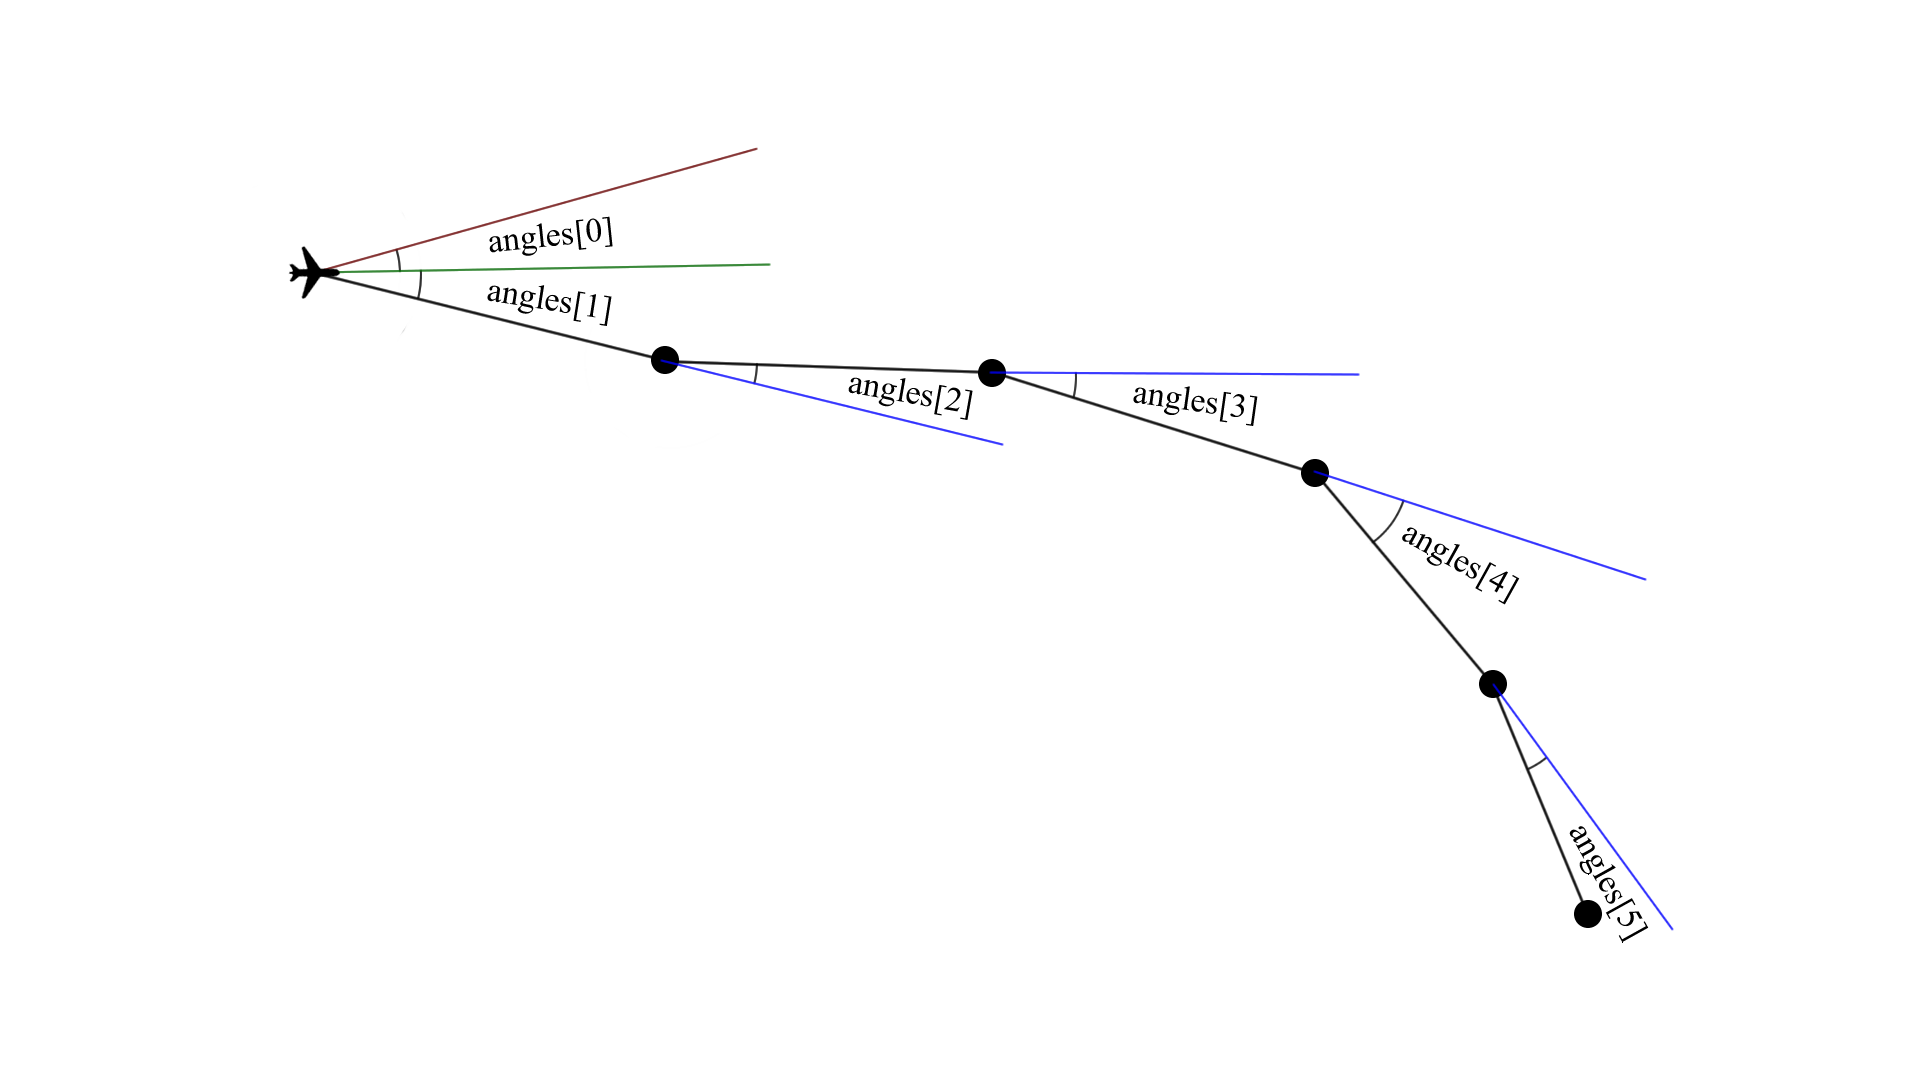
\includegraphics[width=1\textwidth]{angles}
    \caption{Schemat kątów zawartych na planowanej trasie samolotu. Linią czerwoną oznaczono rzeczywisty kierunek poruszania się samolotu, linia zielona wskazuje jego zwrot.}
    \label{fig:katy}
\end{figure}

\textbf{Uwaga:} zgodnie z założeniem projektowym, wszystkie waypointy znajdują się na tej samej wysokości. Z perspektywy programu możliwe by było wprowadzenie trzeciej zmiennej pozycji, jednak podczas lotu manualnego (w trakcie którego zbierane są dane treningowe) oszacowanie wysokości, na której znajduje się samolot jest bardzo nieprecyzyjne i mogło by negatywnie wpłynąć na wynik działania kontrolera.

\begin{figure}[ht]
    \centering
    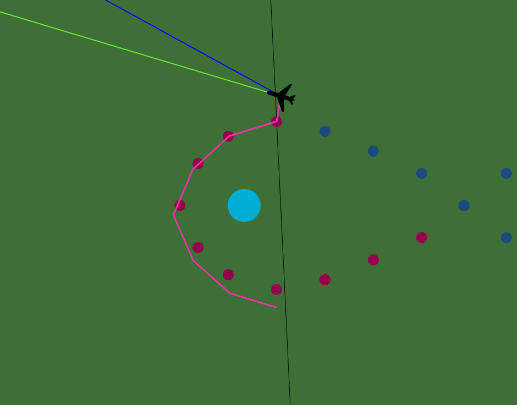
\includegraphics[width=1\textwidth]{estymacja}
    \caption{Trasa oszacowana przy pomocy algorytmu estymacji trajektorii (różowa linia). Linia niebieska wskazuje kierunek rzeczywistego poruszania się samolotu, a linia zielona jego zwrot.}
    \label{fig:estymacja}
\end{figure}

 \FloatBarrier
\subsection{Stacja odbiorcza}
Wszystkie dane wysyłane przez moduł radiowy z pokładu samolotu są odbierane przez ten sam układ HC-12 znajdujący się w naziemnej stacji odbiorczej, w skład której wchodzi jeszcze mikrokontroler Arduino Mega, jak widać na zdjęciu \ref{fig:baza}. Posiada on kilka wbudowanych portów UART, dlatego idealnie nadaje się jako przekaźnik sygnału do portu USB na komputerze.

 \begin{figure}[ht]
    \centering
    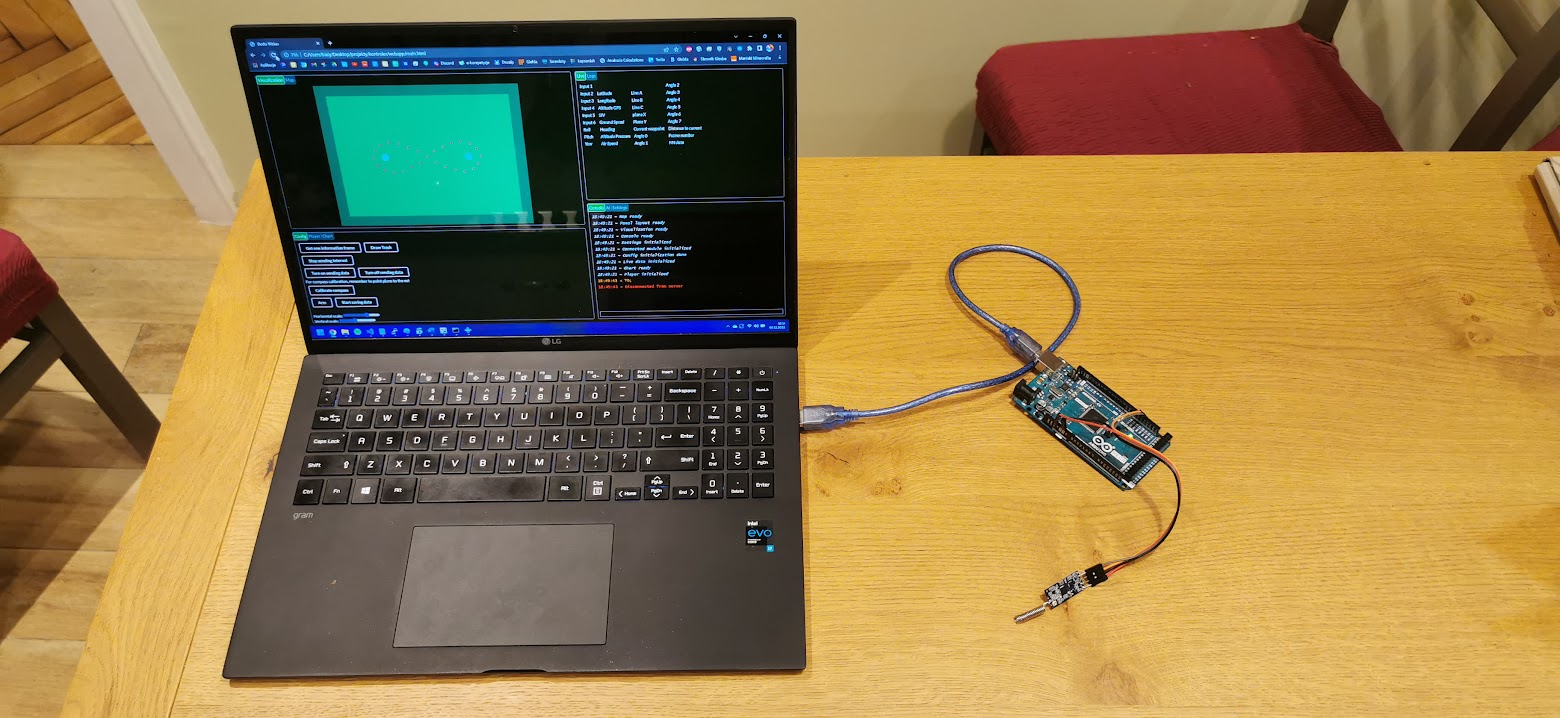
\includegraphics[width=1\textwidth]{baza}
    \caption{Stacja odbiorcza: moduł HC-12, Arduino Mega, laptop z uruchomioną aplikacją przekaźnikową oraz oprogramowanie do wizualizacji danych.}
    \label{fig:baza}
\end{figure}

Programem obsługującym dwustronną komunikację ze stacją odbiorczą jest przygotowany w języku Python3 skrypt, który nasłuchuje zarówno wiadomości od serwera oraz z Arduino i przekazuje je dalej, w odpowiednim kierunku. Wspomniany serwer jest natomiast aplikacją stworzoną w środowisku NodeJS, w języku JavaScript. Działa on jako serwer komunikacji w protokole WebSocket, umożliwiającym praktycznie natychmiastową komunikację pomiędzy podłączonymi wcześniej klientami. Jego zadaniem jest zdekodowanie odbieranych danych i przekazanie do miejsc docelowych. Dzięki temu webowa aplikacja może być uruchomiona jednocześnie na kilku komputerach. Magazynuje także dane zbierane podczas lotu w formie plików dostępnych do pobrania. Serwer ten mógłby zostać uruchomiony w sieci lokalnej (na przykład na laptopie, do którego podłączona jest stacja odbiorcza), jednak w praktyce wygodniejsze okazało się zainstalowanie jej na domowym serwerze, do którego dostęp jest przez sieć Internet. Wspomniany serwer jest urządzeniem z systemem operacyjnym Ubuntu 16.04. Dostęp do niego możliwy jest dzięki statycznemu adresowi IP w sieci lokalnej oraz skorzystaniu z usługi DDNS (Dynamic Domain Name System), która pozwala na przypisanie domeny do zmieniającego się adresu IP routera w sieci globalnej. Stuktura połączeń oraz przepływu informacji w środowisku została pokazana na schemacie \ref{fig:env}

 \begin{figure}[ht]
    \centering
    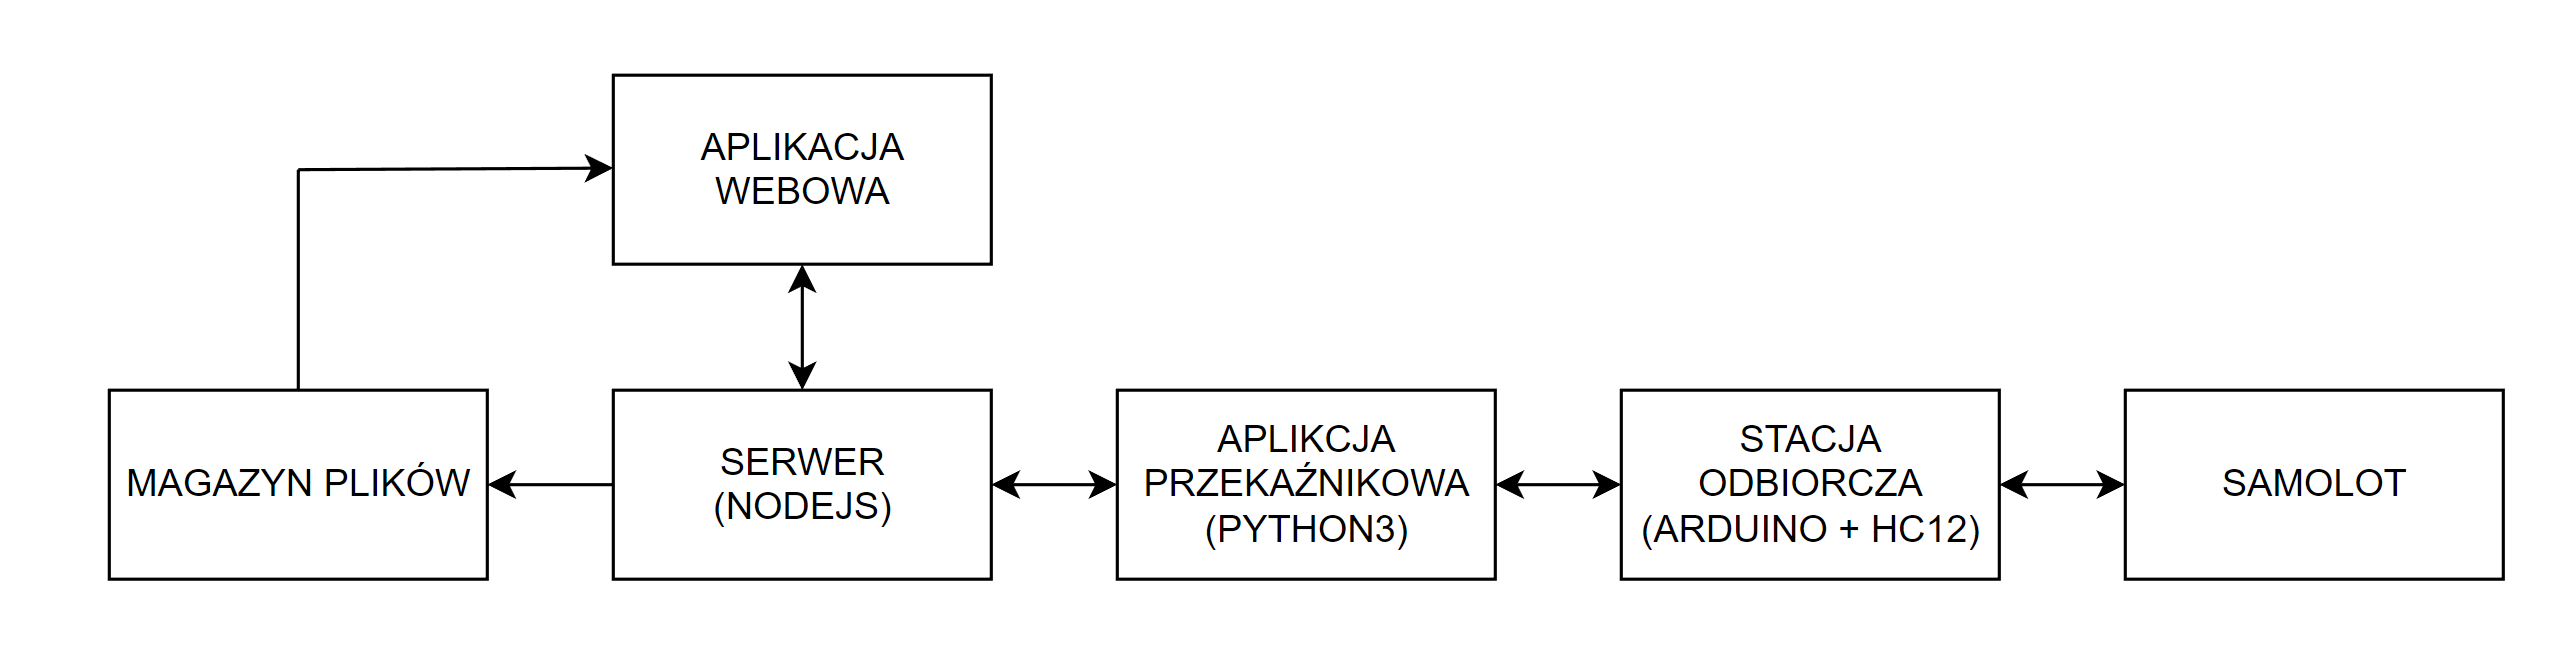
\includegraphics[width=1\textwidth]{diagram_env}
    \caption{Schemat przepływu danych i połączeń w środowisku kontrolera.}
    \label{fig:env}
\end{figure}

Warto wspomnieć, że komunikacja odbywa się przez moduły HC-12, które są transceiverami (połączeniem transmittera oraz receivera), czyli umożliwiają komunikację dwustronną. Moduł ten ma pewne ograniczenia, widoczne przede wszystkim przy próbie równoczesnego nadawania oraz odbierania danych. Po uruchomieniu transmisji, samolot nadaje informacje w trybie ciągłym, dlatego wysłanie do niego poleceń jest bardzo utrudnione i mało prawdopodobne. Z tego powodu na aparaturze jeden z przełączników działa jako blokada transmisji danych od strony oprogramowania kontrolera, która umożliwia zatrzymanie wysyłania oraz bezproblemowe odbieranie informacji.

\FloatBarrier
\subsection{Protokół komunikacji}
Komunikacja między poszczególnymi elementami systemu wymagała opracowania dedykowanego protokołu komunikacyjnego tak, aby każda wiadomość trafiła w odpowiednie miejsce i została prawidłowo odczytana. 

Komunikacja pomiędzy stroną internetową, serwerem i aplikacją przekaźnikową odbywa się przy pomocy ramek w notacji JSON. Wiadomość zawiera pole \textit{type}, oznaczające rodzaj wiadomości - na tej podstawie poszczególne programy wiedzą w jaki sposób odczytać resztę informacji. Poszczególne ramki zawierają dodatkowe pola z informacjami. 

Komunikacja między samolotem a stacją naziemną narażona jest na zakłócenia spowodowane odległością oraz brakiem dodatkowego kodowania wiadomości. Dlatego ramki muszą być maksymalnie krótkie, a algorytm je odczytujący odporny na otrzymanie niekompletnej informacji. Przygotowane zostały trzy typy wiadomości:

\begin{enumerate}
	\item Zapytanie o wartość - składające się ze znaku ? oraz docelowej zmiennej
	\item Nakaz zmiany wartości - składający się ze znaku !, docelowej zmiennej oraz nowej wartości w postaci liczby zmiennoprzecinkowej
	\item Nakaz wykonania akcji - składający się ze znaku @ oraz numeru akcji.	
\end{enumerate}

Każda liczba musi być zakończona symbolem średnika. Poszczególne znaki (w tym także cyfry) są kodowane w postaci znaków ASCII, co zmniejsza ryzyko wystąpienia błędu odczytu informacji - ramka prędzej zostanie utracona niż błędnie zinterpretowana. W odpowiedzi na zapytania o wartości lub przy różnych akcjach samolot może wysłać ramkę zwrotną w postaci: \#, kod informacji, wartość. Kodowane w ten sposób wiadomości są istotne z punktu widzenia pozostałych programów w środowisku. Wiadomości o charakterze informacyjnym mogą zostać wysłane w postaci zwykłego tekstu, który zostanie wyświetlony na konsoli w aplikacji internetowej. Poniżej zamieszczono przykładowe ramki danych: 

?3; - podaj lokalizację lewej kolumny

!0;1; - zmień tryb wysyłania danych na ciągły

@0; - uzbrój samolot

\#5;1; - potwierdzenie prawidłowej inicjalizacji modułu GPS

\FloatBarrier
\subsection{Oprogramowanie naziemne}
Podczas testów samolotu bardzo szybko okazało się, że do efektywnej pracy nad modułem kontrolera konieczne będzie przygotowanie środowiska, które pozwoli na podgląd i wizualizację danych oraz konfigurację parametrów systemu. Początkowy projekt założył prosty program do wyświetlania zapisanych w pliku danych zebranych podczas przelotu w postaci wykresów (rysunek \ref{fig:staryprogram}).

 \begin{figure}[ht]
    \centering
    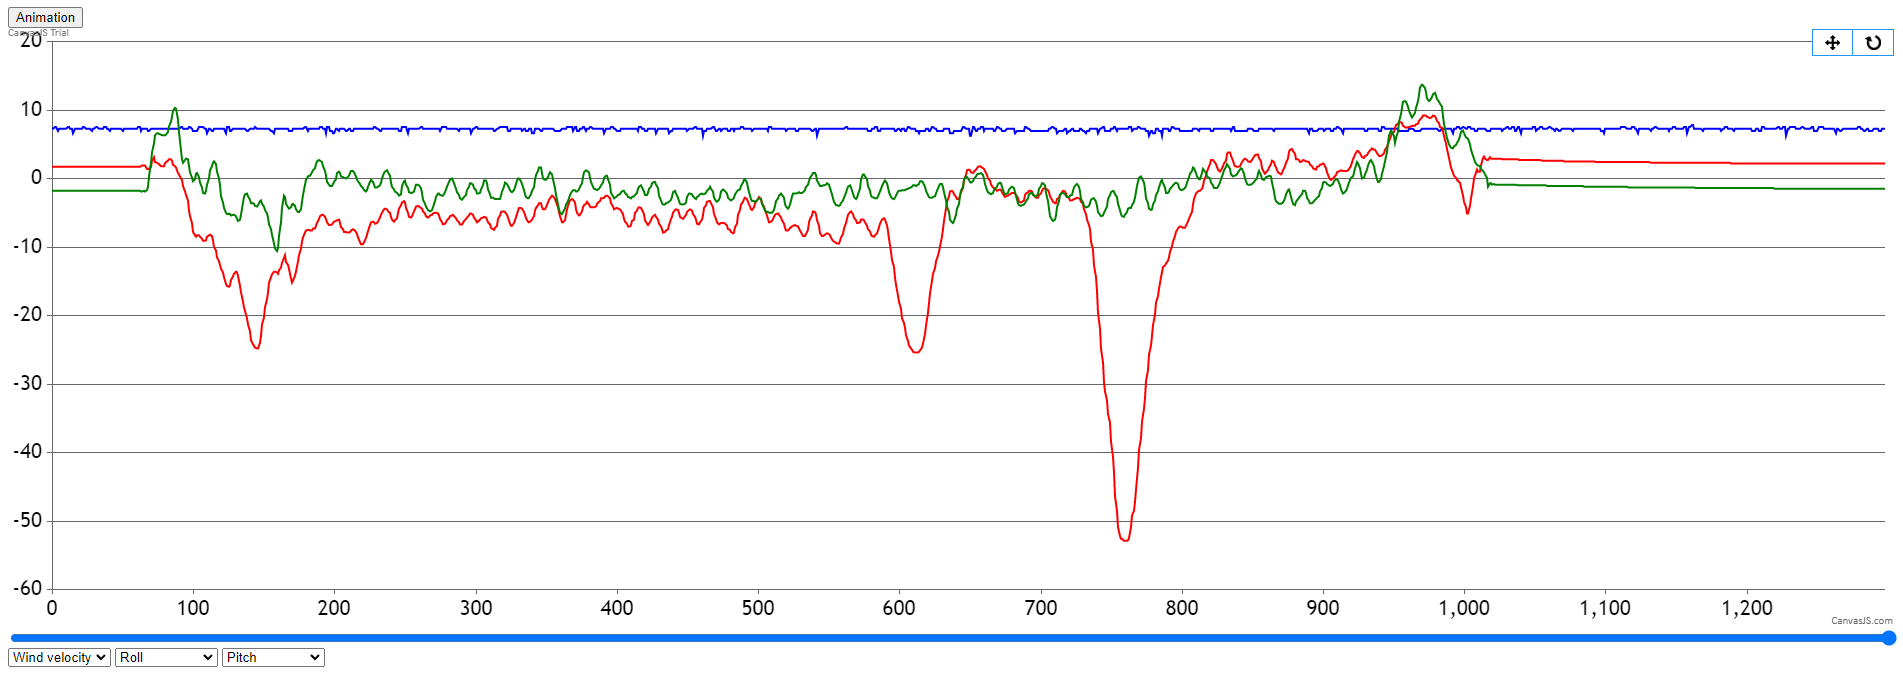
\includegraphics[width=1\textwidth]{starysystem}
    \caption{Pierwsze oprogramowanie pozwalające na wizualizację danych w postaci wykresów.}
    \label{fig:staryprogram}
\end{figure}

Program został przygotowany w formie strony internetowej tak, aby możliwy był do niego dostęp z poziomu przeglądarki. Niestety, szybko okazało się, że jest to rozwiązanie tylko tymczasowe - brak możliwości podglądu danych w czasie rzeczywistym znacząco utrudniał pracę nad samym kontrolerem - największym problemem był brak możliwości sprawdzenia poprawności działania algorytmów przetwarzające dane lokalizacyjne i estymacji trajektorii lotu. Ponadto podczas testów w warunkach polowych bardzo uciążliwa była konieczność ponownej kompilacji całego programu i wgrywania do mikrokontrolera przy każdej zmianie parametrów. 

Pojawił się więc pomysł stworzenia aplikacji, która pozwoli na podgląd danych w czasie rzeczywistym, konfigurację samolotu oraz zapis i analizę zebranych danych. Projektując system największy nacisk położony został na jego przejrzystość, łatwość obsługi i praktyczność tak, aby pozwolić zaoszczędzić każdą cenną sekundę podczas wykonywania lotów testowych. Ekran główny wykonanej aplikacji można zobaczyć na zdjęciu \ref{fig:weball}.

 \begin{figure}[ht]
    \centering
    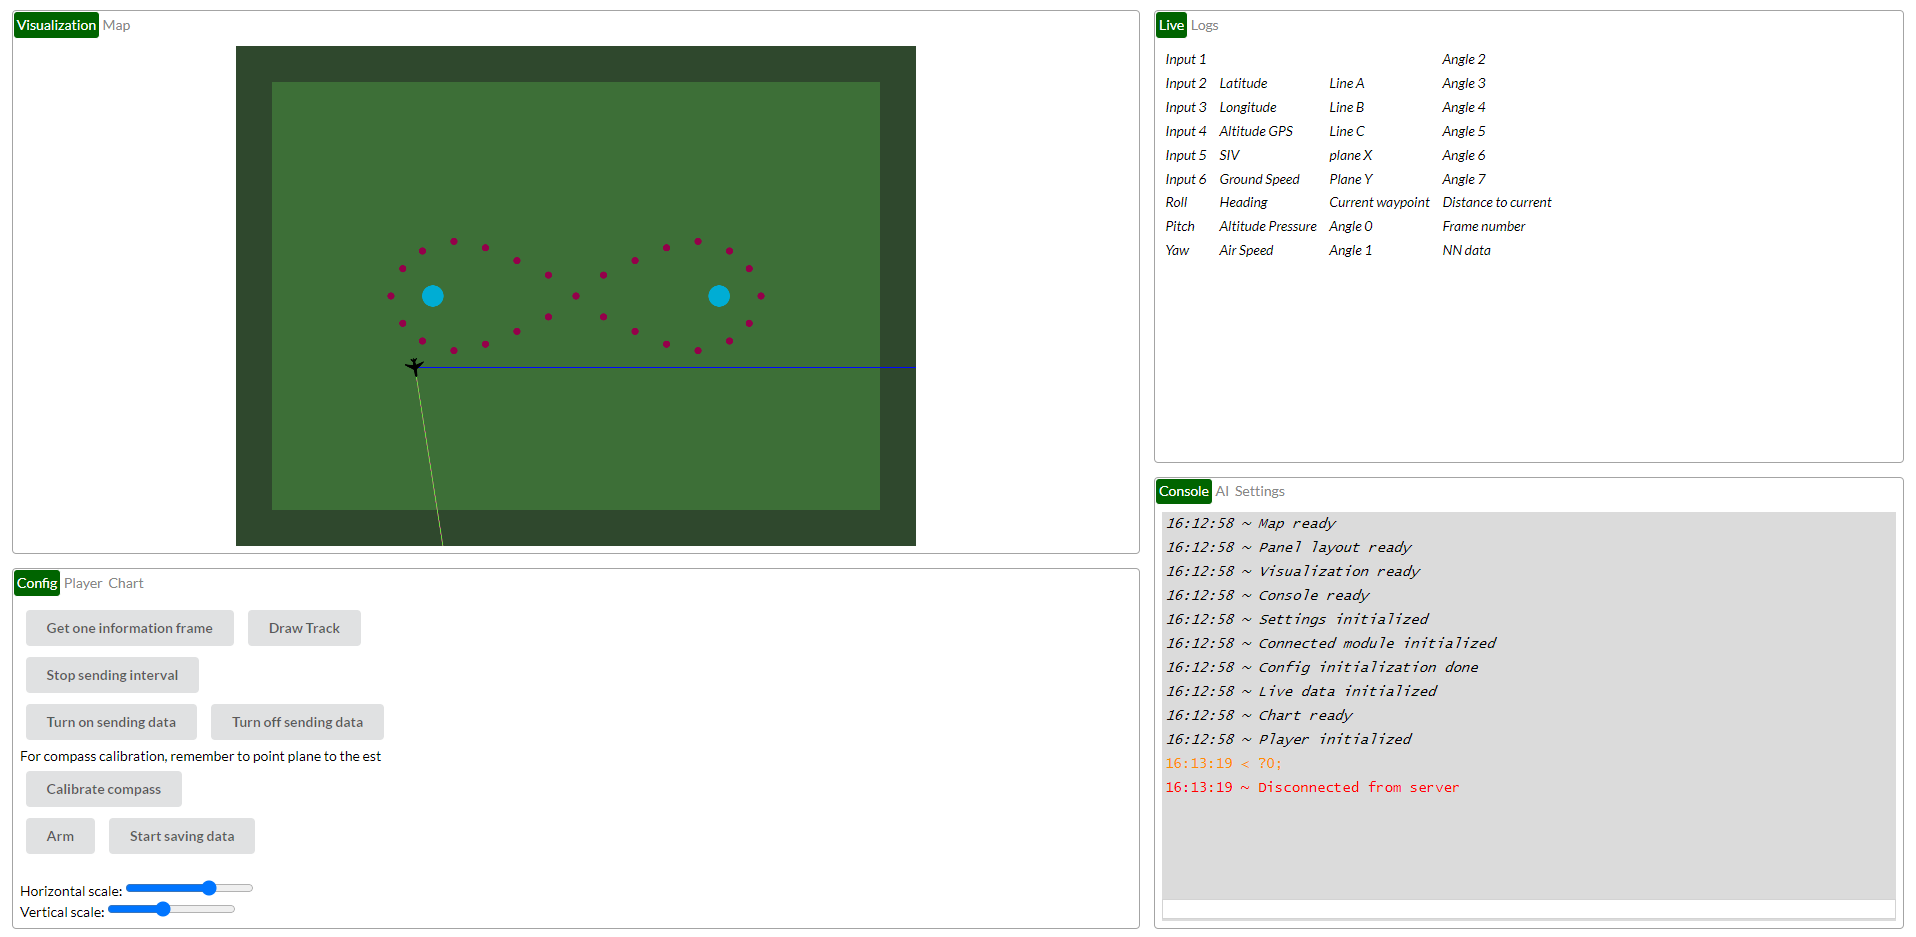
\includegraphics[width=1\textwidth]{weball}
    \caption{Ekran główny aplikacji do przetwarzania danych z kontrolera lotu.}
    \label{fig:weball}
\end{figure}

\paragraph{Układ czteropanelowy}\mbox{}

Wygląd i układ programu są najistotniejszymi elementami decydującymi o jego przejrzystości. Najważniejszym zadaniem podczas projektowania tego typu oprogramowania jest zmaksymalizowanie ilości informacji, które użytkownik może równocześnie obserwować. Zgodnie z założeniem program  miał umożliwiać pracę nad różnymi aspektami kontrolera lotu: analizę danych (w czasie rzeczywistym lub odtworzonych z pliku), konfigurację trasy czy podgląd stanu połączenia całego środowiska. Podsumowując, jedno statyczne ułożenie elementów interfejsu byłoby niemożliwe, stąd koncepcja rozwoju dynamicznego układu czteropanelowego, która pozwala na wyświetlanie różnych stron aplikacji w oknach.

Co najważniejsze, rozmiar paneli nie jest stały, można go dynamicznie modyfikować w intuicyjny sposób, przy pomocy przeciągnięcia wskaźnikiem myszy. Ponadto, strony nie są przypisane do jednego panelu, można zmieniać ich lokalizację po przeciągnięciu paska tytułowego na inny obszar. Zmiana kolejności wyświetlanych stron w obrębie panelu także jest możliwa w analogiczny sposób. Całość umożliwia, w zależności od potrzeby, wyświetlanie na ekranie zupełnie innych zestawów informacji. Przełączenie się między dowolną konfiguracją zajmuje czas liczony w sekundach. Podczas kalibracji przed startem wygodniejszy będzie podgląd na mapę, sieć połączeń środowiska, ekran konfiguracji i konsolę (grafika \ref{fig:web1}), w trakcie lotu niezbędny jest ekran podglądu danych i wizualizacja (grafika \ref{fig:web2}), a podczas analizy zebranych danych panel odtwarzania czy lista plików (grafika \ref{fig:web3}).

System został stworzony w formie strony internetowej przy pomocy technologii: HTML, JavaScript, jQuery, jQuery-UI, Semantic-UI oraz CSS i jest dedykowany do przeglądarki Google Chrome. Dostęp do niego nie wymaga żadnej instalacji i jest możliwy za pośrednictwem Internetu pod adresem:

\begin{center}
\url{http://dodo.jkostecki.pl}
\end{center}

 \begin{figure}[ht]
    \centering
    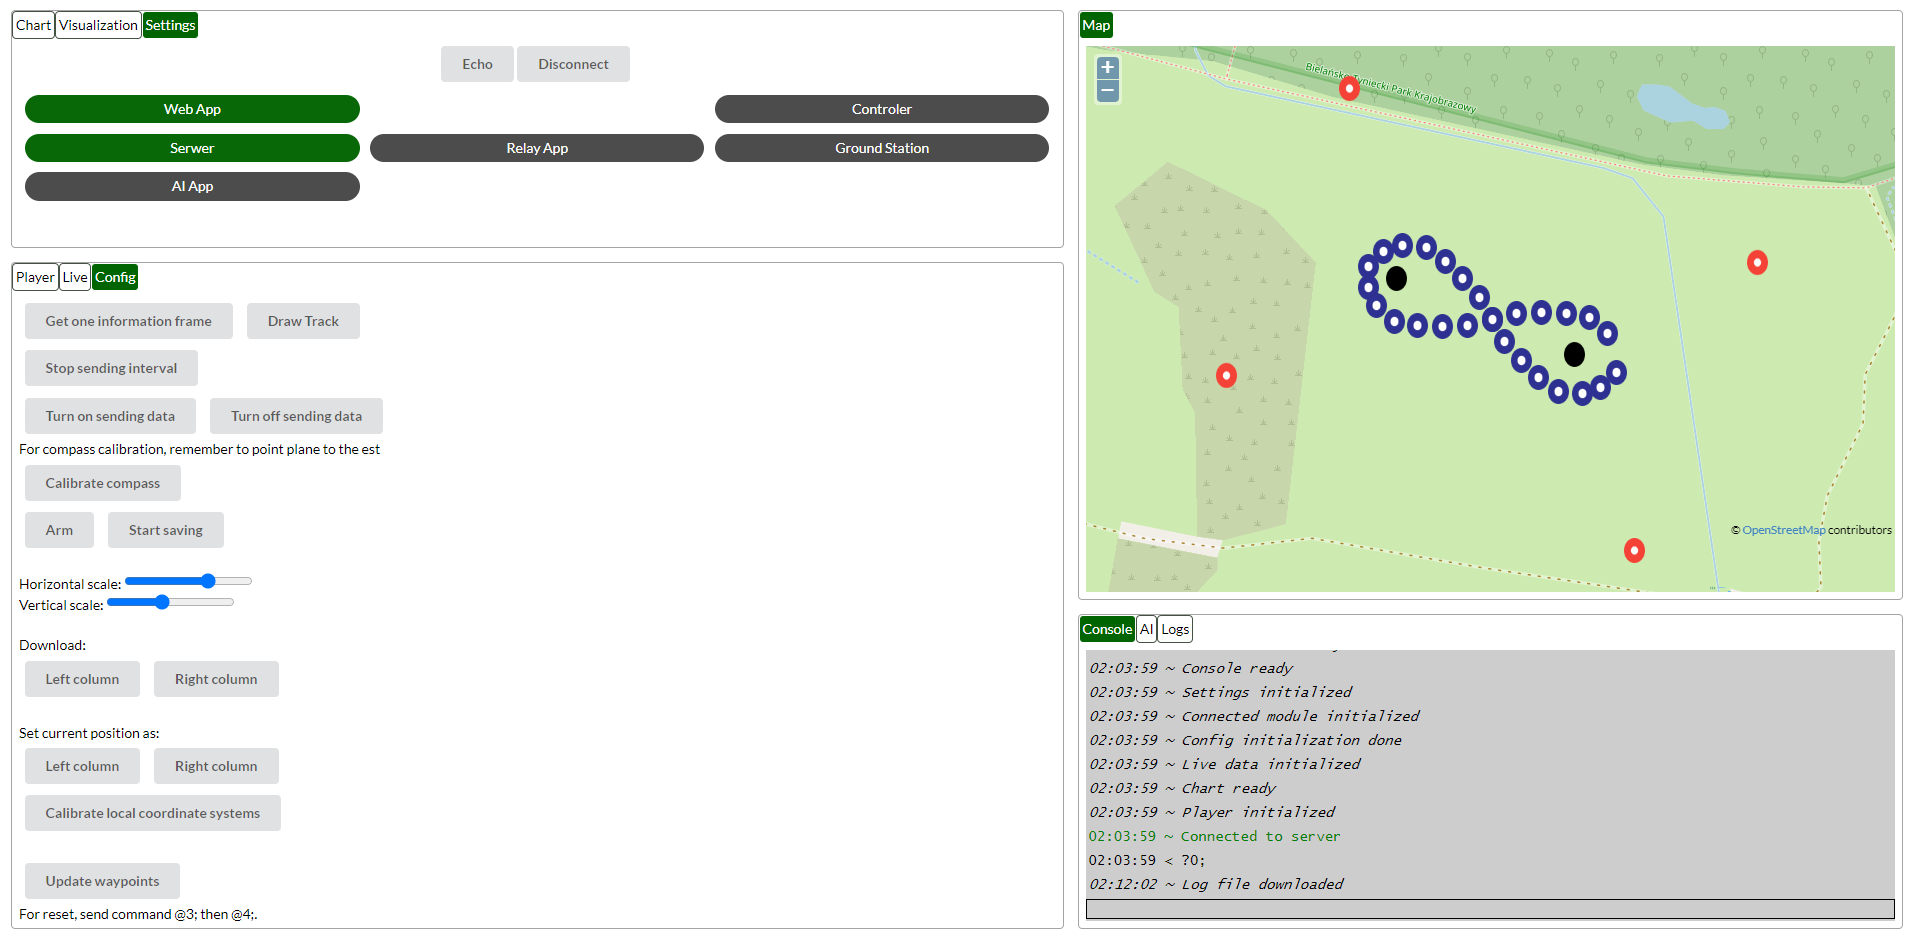
\includegraphics[width=1\textwidth]{przedlotem}
    \caption{Aplikacja w przykładowej konfiguracji do kalibracji przed startem.}
    \label{fig:web1}
\end{figure}

 \begin{figure}[ht]
    \centering
    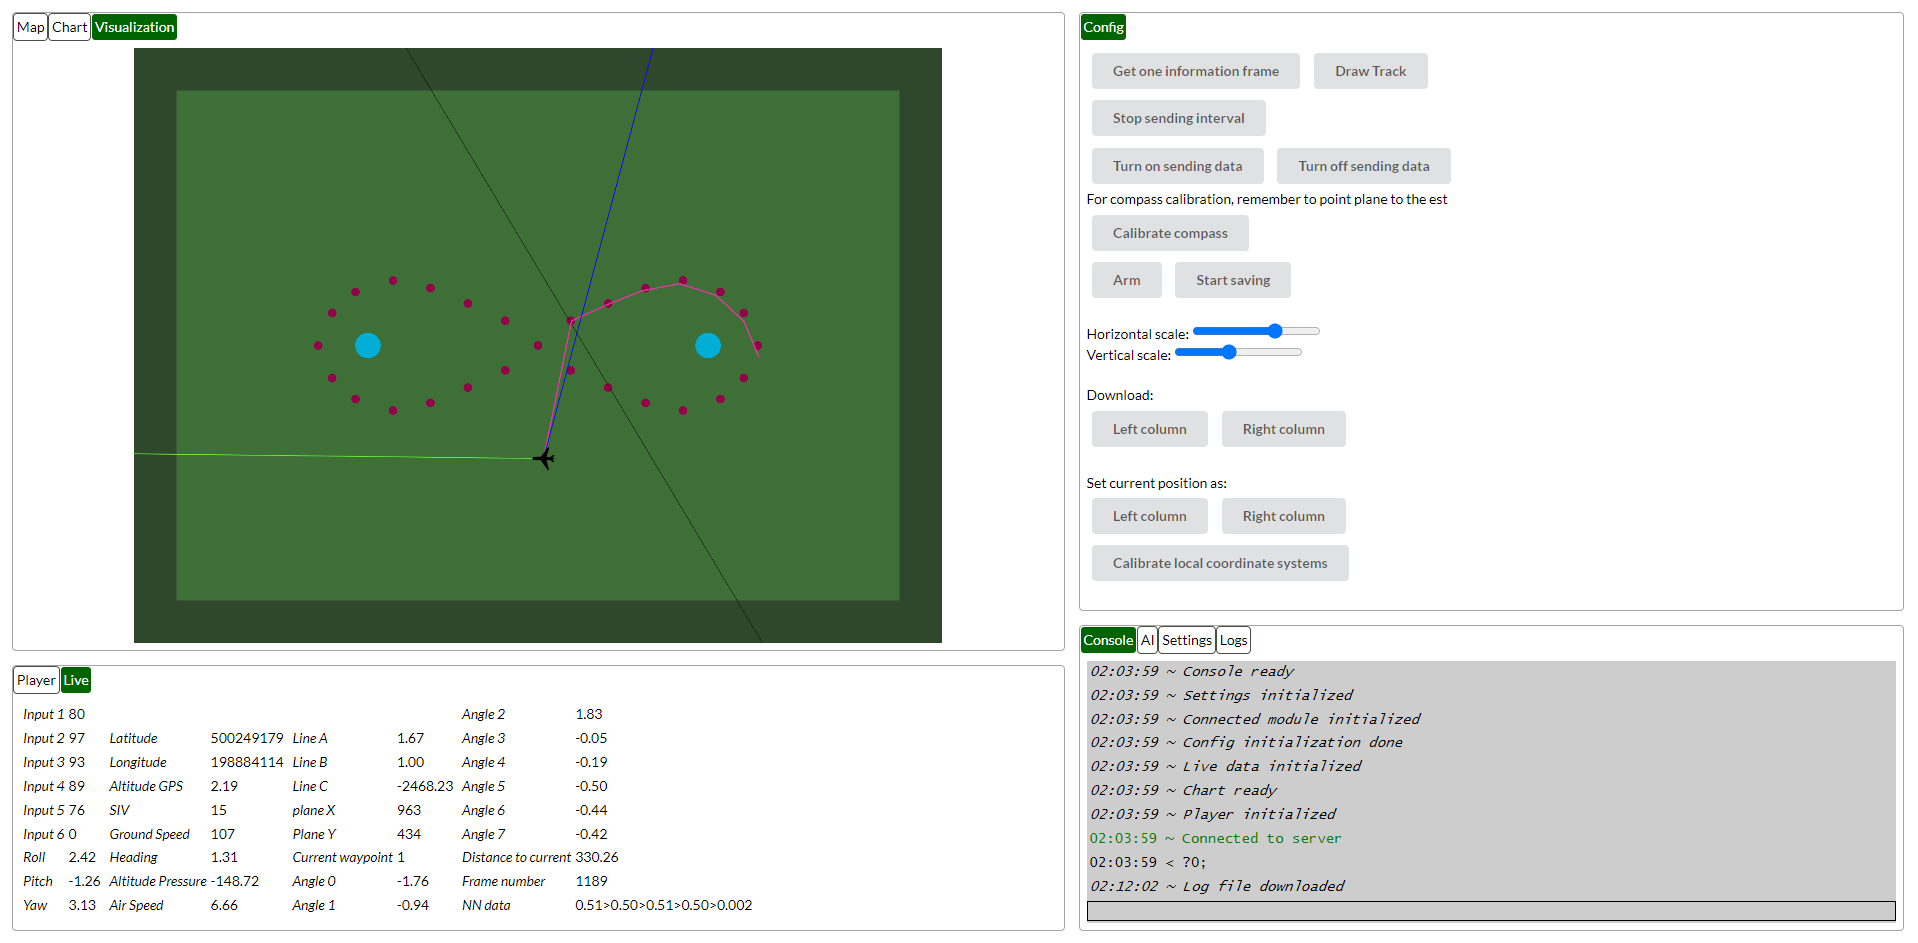
\includegraphics[width=1\textwidth]{podczaslotu}
    \caption{Aplikacja w przykładowej konfiguracji do obserwacji lotu.}
    \label{fig:web2}
\end{figure}

 \begin{figure}[ht]
    \centering
    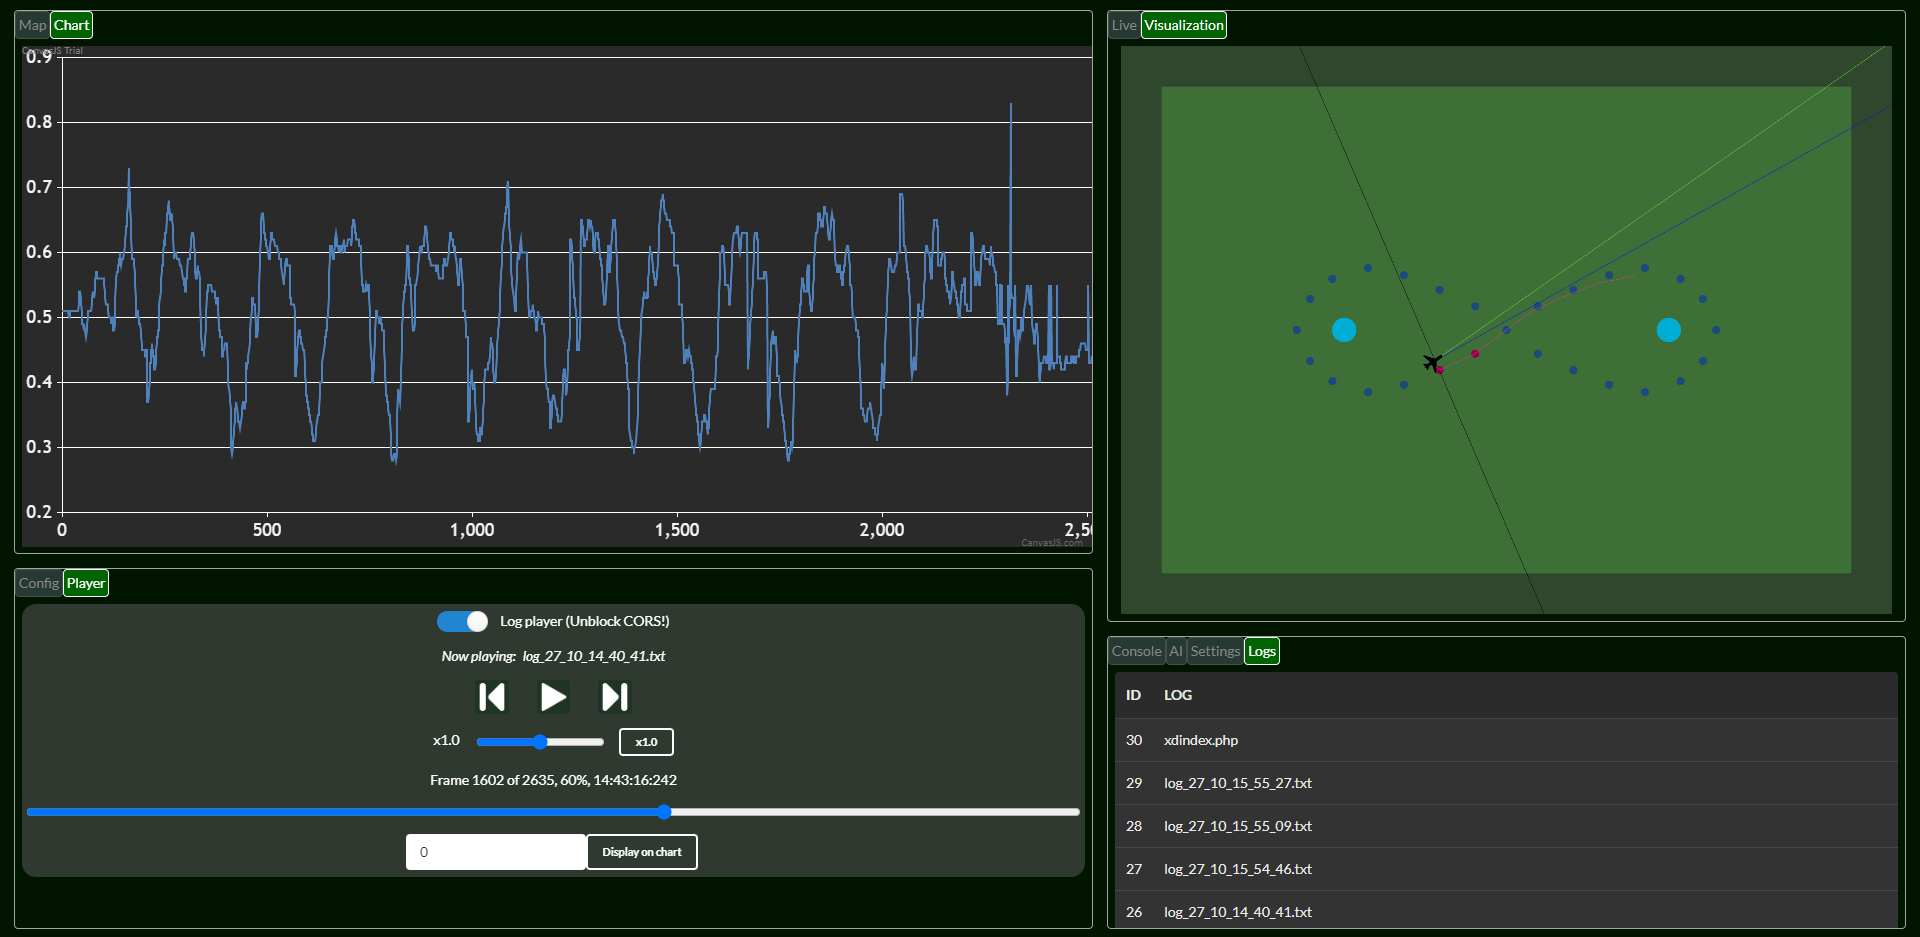
\includegraphics[width=1\textwidth]{polocie}
    \caption{Aplikacja w przykładowej konfiguracji do analizy danych.}
    \label{fig:web3}
\end{figure}

\FloatBarrier
 
\paragraph{Strona: Wizualizacja}\mbox{}

Strona wizualizacji jest jedną z najistotniejszych zakładek pozwalających sprawdzić obecne położenie samolotu, wyznaczoną trasę, waypointy oraz informację, które z nich zostały już zaliczone. Podczas tworzenia algorytmów transformacji do lokalnego układu współrzędnych oraz estymacji trajektorii podgląd taki okazał się niezbędny, zwłaszcza na etapie weryfikacji poprawności ich działania - dane liczbowe często mogły się wydawać poprawne, jednak dopiero ich wizualizowanie pozwoliło na bardzo dokładne sprawdzenie i wychwycenie błędów - przykładem może być niepoprawne skalowanie względem osi układu. W trakcie lotu testowego podgląd pozycji jest także wygodny jako wsparcie pilota, który nie zawsze jest w stanie poprawie określić odległość samolotu od siebie. Ponadto, możliwe jest sprawdzenie w czasie rzeczywistym kalibracji i poprawności danych z czujnika orientacji. Do korzystania z modułu wizualizacji konieczna jest kalibracja lokalnego układu współrzędnych z samolotem. 

Bezpośrednio powiązaną stroną jest moduł wyświetlania danych w czasie rzeczywistym, które są aktualizowane na podstawie ramek przychodzących z samolotu. Obie te strony widoczne są na grafice \ref{fig:wizlive}

 \begin{figure}[H]
    \centering
    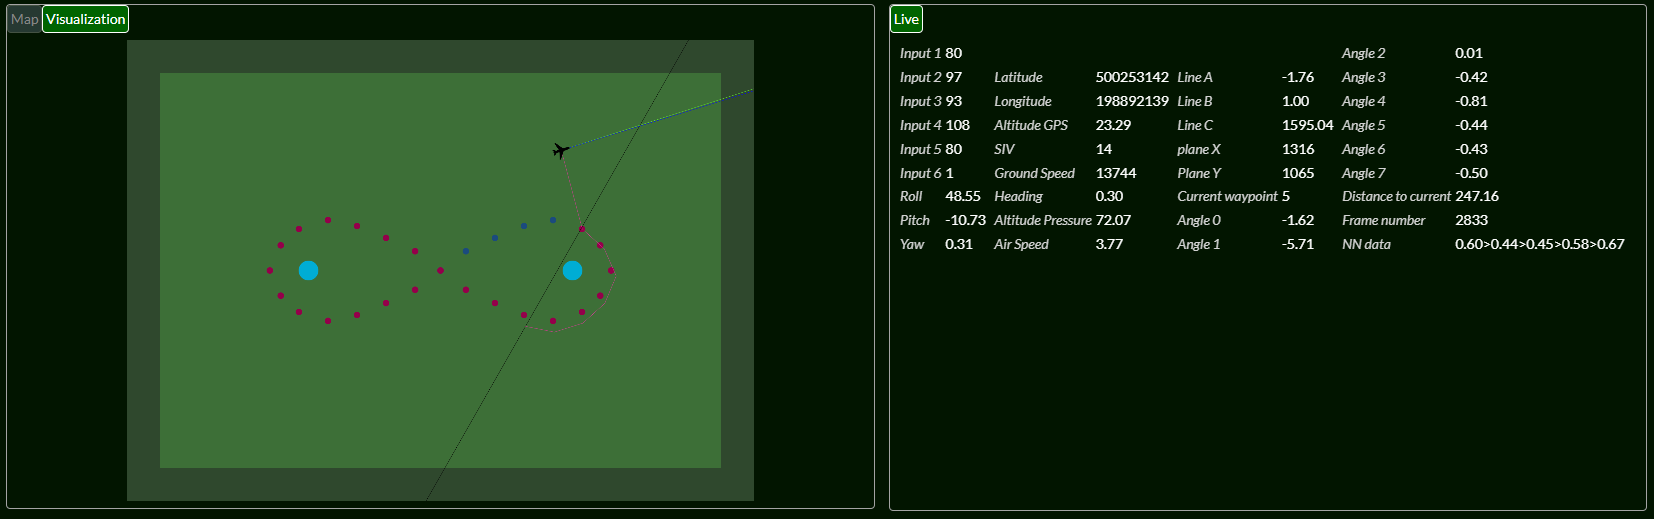
\includegraphics[width=1\textwidth]{wizualizacja}
    \caption{Strona wizualizacji oraz strona danych w czasie rzeczywistym.}
    \label{fig:wizlive}
\end{figure}

\paragraph{Strona: Mapa}\mbox{}

Podczas przygotowań do startu i przy wyznaczeniu obszaru lotu oraz jego trasy, pomocne może być określenie położenia samolotu na mapie terenu. W tym celu wykorzystano działające na licencji open-source Open Street Maps poprzez bibliotekę OpenLayers. Na mapie naniesiona jest lokalizacja samolotu a także kolumny, waypointy oraz granice obszar lotu (grafika \ref{fig:mapa}).

 \begin{figure}[H]
    \centering
    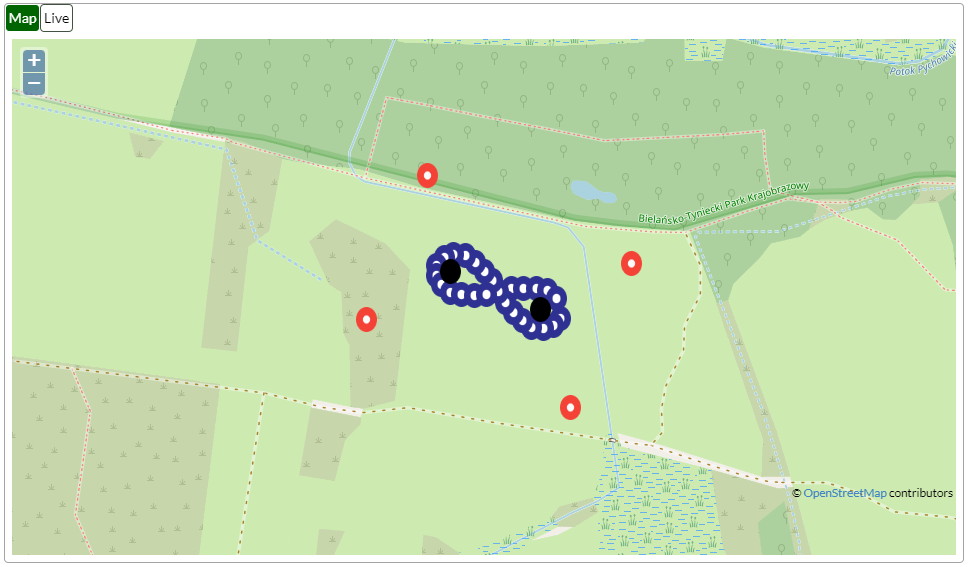
\includegraphics[width=1\textwidth]{mapa}
    \caption{Strona mapy terenu z naniesionymi punktami.}
    \label{fig:mapa}
\end{figure}


\paragraph{Strona: Konsola}\mbox{}

Konsola została przygotowana z myślą o bezpośredniej dwustronnej komunikacji z kontrolerem, a także wyświetlania komunikatów z całego środowiska. Tekst wpisany w wejście konsoli zostaje wysłany bezpośrednio do kontrolera. Interakcja z konsolą odbywa się w sposób analogiczny jak w najczęściej używanych tego typu aplikacjach - zaimplementowana została możliwość korzystania ze strzałek do przewijania poprzednio wysłanych komend, automatyczne przewijanie do nowych wiadomości po ręcznym przewinięciu na sam dół, a okno wpisywania staje się aktywne po kliknięciu gdziekolwiek na obszarze panelu. Dodatkowo wyświetlany tekst może być odpowiednio stylizowany oraz pokazywane jest jego źródło poprzez odpowiedni symbol przed wiadomością, jak widać na grafice \ref{fig:konsola}. Konsola przechowuje do 1000 wierszy informacji.

 \begin{figure}[H]
    \centering
    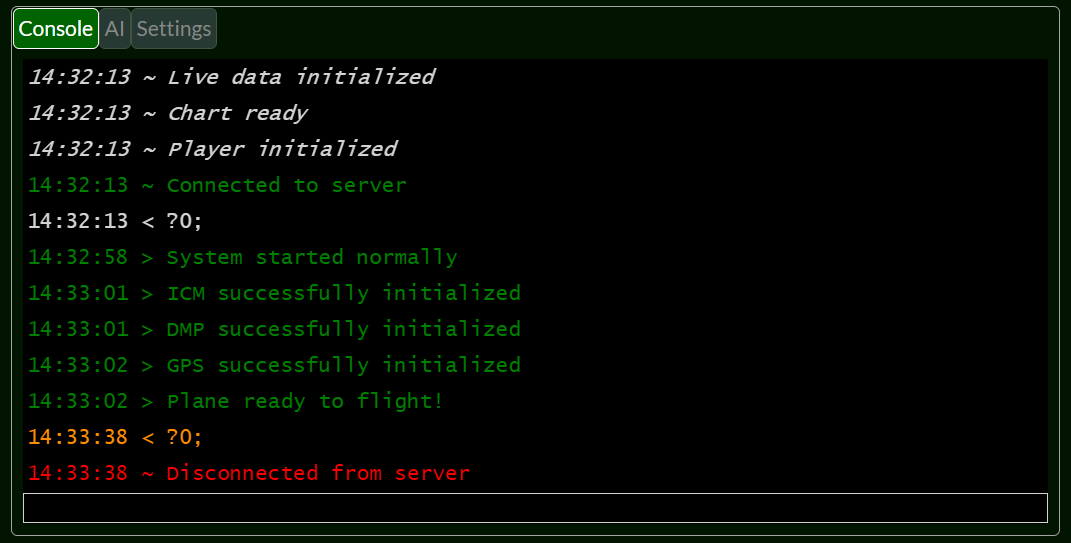
\includegraphics[width=1\textwidth]{konsola}
    \caption{Strona konsoli do bezpośredniej komunikacji z kontrolerem.}
    \label{fig:konsola}
\end{figure}

\paragraph{Strona: Konfiguracja}\mbox{}

Strona ta jest kluczowa przy konfiguracji samolotu przed startem. Umożliwia zarządzenie wysyłaniem danych, zbrojeniem silnika, zapisem danych, kalibracją terenu czy zarządzaniem trasą. Dzięki użyciu protokołu komunikacyjnego możliwe jest automatyczne wysłanie danych, wraz z informacją zwrotną - przykładowo potwierdzenie poprawnego odebrania pozycji waypointa skutkuje uruchomieniem procedury wysłania kolejnego, aż do końca listy. Ekran konfiguracji składa się głównie z przycisków, jak widać na grafice \ref{fig:konlog}

 \begin{figure}[H]
    \centering
    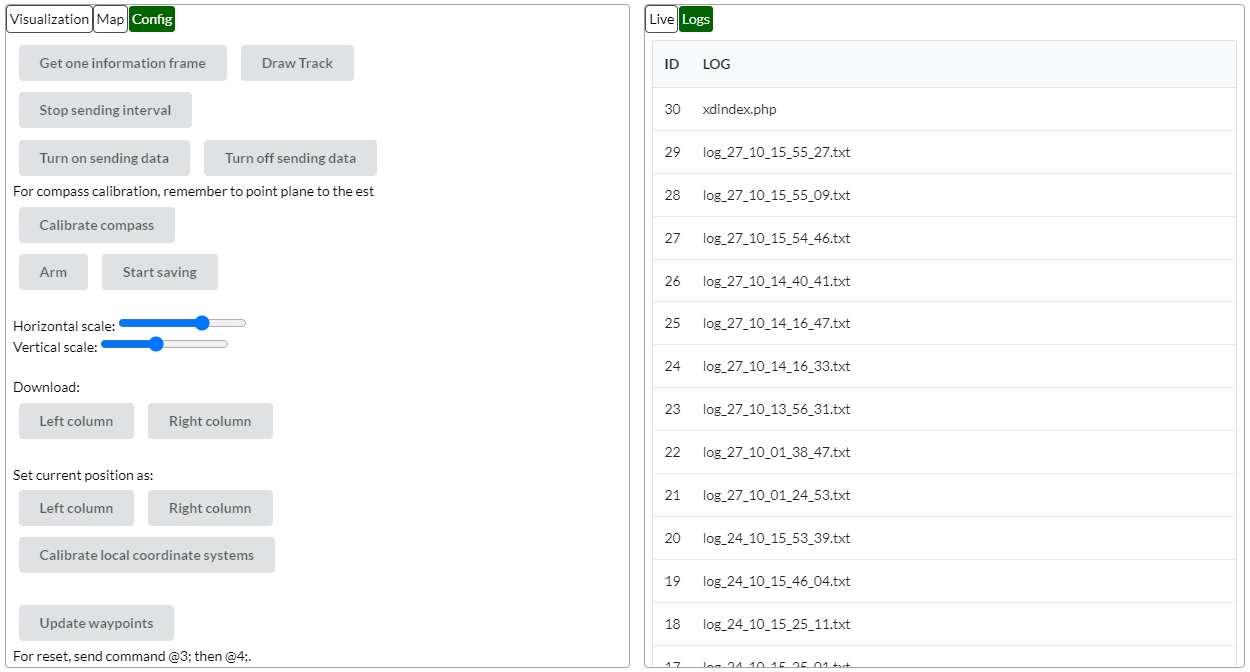
\includegraphics[width=1\textwidth]{config}
    \caption{Strona konfiguracji oraz lista zapisanych logów z lotów.}
    \label{fig:konlog}
\end{figure}

\paragraph{Strona: Ustawienia}\mbox{}

Jeżeli nie powiedzie się próba podłączenia aplikacji do samolotu, najszybszym sposobem zlokalizowania problemu jest zakładka ustawień - za pomocą mapy połączeń w całym środowisku możliwe jest określenie miejsca występowania błędu. Na grafice \ref{fig:settings} wszystkie elementy na drodze między aplikacją internetową a samolotem są podświetlone na kolor zielony, co oznacza poprawne połączenie. W przypadku wystąpienia błędu - dla przykładu rozłączenia aplikacji przekaźnikowej - jej pole i wszystkie po nim następujące wyłączą podświetlenie, zatem od razu widać, który element nie działa. Wywołanie funkcji Echo skutkuje wysłaniem prośby do kolejnych programów o odesłanie informacji zwrotnej o prawidłowym działaniu. Podczas prac strona okazała się bardzo praktyczna i pozwoliła każdorazowo na oszczędzenie nawet kilku minut na szukanie błędów. 

\textbf{Uwaga:} z przyczyn praktycznych aplikacja do treningu sztucznej inteligencji ostatecznie nie została podłączona do środowiska.

 \begin{figure}[H]
    \centering
    \includegraphics[width=1\textwidth]{settings}
    \caption{Strona ustawień aplikacji w sytuacji prawidłowej komunikacji z kontrolerem.}
    \label{fig:settings}
\end{figure}

\paragraph{Strona: Odtwarzacz}\mbox{}

Strona odtwarzacza pozwala na podgląd zapisanych plików z danymi z przelotów (lista dostępnych plików znajduje się w zakładce z logami - grafika \ref{fig:konlog}). Jest niezwykle istotna podczas analizy przelotów. Jak można zauważyć na grafice \ref{fig:player}, dostępne jest odtwarzanie i pauzowanie, przesuwanie pojedynczych klatek, dostosowanie prędkości odtwarzania (w zakresie od 0.1 do 10 razy) oraz przewijanie przy pomocy suwaka. Dodatkowo wybrane dane można wyświetlić na wykresie. Informacje z plików pokazywane są na ekranie wizualizacji oraz w zakładce z danymi w czasie rzeczywistym.

 \begin{figure}[H]
    \centering
    \includegraphics[width=1\textwidth]{player}
    \caption{Odtwarzacz zapisanych danych z przelotów.}
    \label{fig:player}
\end{figure}

\FloatBarrier
\subsection{Trening sieci neuronowej}
Przygotowania wszystkich elementów wymienionych w poprzednich rozdziałach okazało się niezbędne do przejścia do procesu nauczania maszynowego. Sprawdzenie niezawodności poszczególnych systemów i poprawności informacji pozwoliło na przystąpienie do zbierania danych treningowych.

W celu przygotowania algorytmów sztucznej inteligencji pierwszym krokiem było określenie wyboru algorytmu przetwarzania danych - wybór padł na rekurencyjną sieć neuronową, ze względu na sposób i możliwość jej nauczania, a także na możliwość rekurencyjnego brania pod uwagę poprzedniej chwili czasowej. Zgodnie z założeniem projektu sterowanie samolotem ma się odbywać w pełni poprzez sztuczną inteligencję - odpowiedź z sieci neuronowej jest kierowana prosto na serwomechanizmy i silnik. 

Kolejnym z założeń projektu było wykorzystanie doświadczenia pilotów w sterowaniu modelami  bezpośrednio do nauki algorytmu sterowania. Lot modelem samolotu jest niezwykle trudnym zadaniem, a wykonanie wielu powtarzalnych przelotów trasy (w tym przypadku "ósemki") wymaga bardzo dużej ilości praktyki. Głównym pilotem samolotu został więc Kacper Krempa, wicemistrz Polski w kategorii lotów modelami F3K oraz wicemistrz Europy w lotach modeli kosmicznych, widoczny na zdjęciu \ref{fig:kacper}.

 \begin{figure}[ht]
    \centering
    \includegraphics[width=1\textwidth]{kacperlata}
    \caption{Lot treningowy samolotem EasyGlider 4.}
    \label{fig:kacper}
\end{figure}


Zadaniem sztucznej inteligencji jest więc zaobserwowanie stanu samolotu w powietrzu w locie manualnym oraz skorelowanie tego stanu z reakcją i zachowaniem pilota, okazywane przez odpowiednie wychyły drążków aparatury. Taka zależność powinna później zostać odtworzona podczas lotu autonomicznego. Aby określić stan samolotu, należy wziąć pod uwagę: wychylenie samolotu w osi roll oraz w osi pitch, wartości tych kątów z poprzedniej chwili czasowej (różnica tych wartości może służyć do stabilizacji), prędkość względem ziemi, wysokość względną (od wysokości startu), prędkość względem powietrza, planowaną trajektorię lotu, a także rekurencyjną odpowiedź sieci z poprzedniej chwili czasowej. Warto zaznaczyć, że użyte serwomechanizmy są z rodziny serwomechanizmów analogowych - nie są one zatem w stanie wysłać informacji zwrotnej o rzeczywistym chwilowym ustawieniu. Jednak przy stosunkowo małych prędkościach zmiany położenia (rzędu kilkunastu stopni w ciągu sekundy) można uznać, że zadane ustawienie odpowiada rzeczywistemu.

Implementacja sieci i efektywny proces nauczania wymaga użycia biblioteki lub innego gotowego środowiska - przygotowanie i przetestowanie programu do treningu sieci przy pomocy algorytmów propagacji wstecznej jest bardzo czasochłonny procesem, a także bezcelowym - istniejące rozwiązania okażą się prawdopodobnie bardziej sprawne i skuteczne. Dlatego po odrzuceniu początkowego pomysłu przygotowania własnego oprogramowania treningowego, zdecydowano się na użycie biblioteki TensorFlow w języku Python3. Umożliwia ona przygotowanie nawet bardzo złożonych algorytmów nauczania maszynowego, w tym także konwolucyjnych sieci neuronowych do przetwarzania obrazów, równocześnie korzystając z mocy obliczeniowej kart GPU. Poprawne zainstalowanie i konfiguracja biblioteki jest dość uciążliwa, problematyczne jest zwłaszcza zainstalowanie sterowników do karty graficznej, jednak po poprawnej instalacji dostępne jest bardzo wygodne środowisko do pracy ze sztuczną inteligencją. W systemie Windows do pracy z wirtualnym środowiskiem wykorzystano oprogramowanie Anakonda. Wykorzystana wersja Pythona to 3.7.9, natomiast wersja TensorFlow to 2.1. Użycie wyższych wersji Pythona nie jest możliwe ze względu na brak kompatybilności z drugą z bibliotek.

Problem sterowania samolotem jest dość liniowo zależny od jego stanu - wychylenie powietrzni sterowych związane jest w dużym stopniu z pozycją samolotu na trasie i planowanej dalszej trajektorii, a także może być wspomagany przez (również w dużym stopniu liniowy) problem stabilizacji. Dlatego wybrana sieć neuronowa nie jest głęboka - posiada 21 wejść, 10 neuronów ukrytych (w jednej warstwie) oraz 5 wyjść (4 serwomechanizmy oraz silnik). Schemat sieci przedstawiono na rysunku \ref{fig:siec}.

 \begin{figure}[H]
    \centering
    \includegraphics[width=1\textwidth]{siec}
    \caption{Schemat wykorzystanej rekurencyjnej sieci neuronowej.}
    \label{fig:siec}
\end{figure}

W bibliotece TensorFlow sieć ta zdefiniowana jest jako model typu Sequential, z przyjętą sigmoidalną funkcją aktywacji oraz definicją błędu pomiarowego jako średni błąd kwadratowy. Do procesu nauczania wykorzystano dane zebrane podczas przelotów treningowych.

Trening został przeprowadzony na podstawie około 1500 chwil czasowych. Po około 35 epokach spadek błędu jest niewielki (wykres \ref{fig:tren1}), dalsze działanie algorytmu może więc skutkować przeuczeniem sieci. Po przetestowaniu działania na przykładowych danych testowych otrzymany wynik predykcji sieci zdaje się być poprawny, zatem sieć można wstępnie uznać za wytrenowaną.

 \begin{figure}[H]
    \centering
    \includegraphics[width=1\textwidth]{tfloss}
    \caption{Krzywa konwergencji średniego błędu kwadratowego w kolejnych epokach treningu sieci z wykorzystaniem TensorFlow.}
    \label{fig:tren1}
\end{figure}

Jedną z wad biblioteki TensorFlow jest brak bezpośredniego dostępu do struktury wytrenowanej sieci neuronowej - macierzy wag połączeń oraz biasów. Sposobem na wygenerowanie modelu jest jego konwersja do pliku typu TFlite. Biblioteka TensorFlowLite jest biblioteką dedykowaną dla urządzeń mobilnych, która umożliwia wykorzystanie modelu na docelowym urządzeniu, takim jak telefon, mikrokontroler czy w aplikacji komputerowej. Modele TFlite są lżejsze oraz zoptymalizowane do pracy z wykorzystaniem mniejszych zasobów obliczeniowych i pamięciowych.

Wersja biblioteki TensorFlowLite dostępna na mikrokontrolery jest kompatybilna ze środowiskiem Arduino IDE. Jednak nie jest ona dostępna dla wszystkich mikroprocesorów, oficjalnie wspierane jest niewiele urządzeń takich jak Arduino Nano 33 BLE Sense, STM32F746 czy ESP-EYE. Mimo braku oficjalnego wsparcia, na wykorzystanym w projekcie Teensy 4.0 (mikroprocesor ARM Cortex-M7) istnieje możliwość uruchomienia biblioteki. Plik z modelem sieci neuronowej TFlite musi uprzednio zostać przemieniony na tablicę znaków w systemie szesnastkowym, która może zostać zinterpretowana przez język C/C++. W tym celu można wykorzystać dostępną w systemach UNIX komendę xdd lub użyć skryptu w Pythonie. Finalnie otrzymany plik można zapisać z rozszerzeniem .h i zaimportować przez kompilator AVR-GCC po stronie środowiska Arduino. Model można poddać dodatkowemu procesowi kwantyzacji, co pozwala jeszcze bardziej ograniczyć jego zapotrzebowanie na moc obliczeniową oraz pamięciową - podczas treningu liczby zmiennoprzecinkowe zapisane są w formacie float64, kwantyzacja pozwala na implementację z wykorzystaniem na przykład postaci float32 czy float16.

Niestety, przykładowych rozwiązań zastosowania modelu TensofFlow na mikrokontrolerach ze szczegółowym opisem ich implementacji jest w Internecie bardzo niewielka ilość, oficjalna dokumentacja również jest skromna i nie zawiera opisu rozwiązań wielu problemów. To wszystko sprawiło, że praca z biblioteką okazała się bardzo uciążliwa. Po wielu próbach udało uruchomić wytrenowaną sieć, jednak problemem okazała się rozbieżność odpowiedzi sieci dla danych testowych w oryginalnej aplikacji uczącej i na mikrokontrolerze. Rozbieżność ta wynika najprawdopodobniej z konieczności skalowania danych wejściowych i wyjściowych (co jest częstą procedurą w implementacji tego typu sieci neuronowych), jednak próby naprawienia tego problemu nie powiodły się. 

Drugim równocześnie testowym oprogramowaniem do uczenia maszynowego było narzędzie Neural Net Fitting App z Deep Learning Toolbox w środowisku Matlab. Jego zdecydowaną przewagą nad biblioteką TensorFlow jest możliwość wyeksportowania macierzy wag i biasów wytrenowanej sieci neuronowej. Dodatkowo istnieje opcja wygenerowania źródłowego kodu do obsługi sieci w języku MATLAB. Wykorzystując tę funkcjonalność przygotowany został skrypt umożliwiający konwersję wytrenowanego modelu - jego struktury i wartości - do pliku .h w języku C++. Na ten sam język przetłumaczone zostały funkcje odpowiadające za propagację sygnału przez sieć, której kolejnymi krokami są:

\begin{enumerate}
    \item Wpisane danych do macierzy wejściowej.
	\item Translacja wejścia o stały offset (odejmowanie).
	\item Skalowanie wejścia o stałą wzmocnienia (mnożenie).
	\item Translacja wejścia o wartość minimalną (dodawanie).
	\item Propagacja do drugiej warstwy:
	\begin{enumerate}
		\item Mnożenie macierzy wejściowej przez macierz wag połączeń.
		\item Translacja o bias.
		\item Transformacja funkcją tangensa hiperbolicznego.
	\end{enumerate}
	\item Propagacja do warstwy wyjściowej:
	\begin{enumerate}
		\item Mnożenie macierzy pierwszej warstwy przez macierz wag połączeń.
		\item Translacja o bias.
	\end{enumerate}
	\item Translacja wyjścia o wartość minimalną (odejmowanie).
	\item Skalowanie wyjścia o stałą wzmocnienia (dzielenie).
	\item Translacja wyjścia o stały offset (dodawanie).
\end{enumerate}

Stałe skalowania i translacji są indywidualne dla każdego neuronu wejściowego i wyjściowego. W pierwszej warstwie ukrytej funkcją aktywacji jest tangens hiperboliczny, w warstwie wyjściowej nie jest użyta funkcja aktywacji, wynik jest tylko liniowy skalowany. Wykorzystany algorytm zwraca taką samą odpowiedź w środowisku treningowym (Matlab) jak i na mikrokontrolerze, osiągnięty zatem został cel implementacji zadanej sieci.

\textbf{Uwaga:} przygotowany algorytm umożliwia automatyczną zmianę ilości neuronów w każdej z warstw. Dopiero modyfikacja struktury sieci (ilości warstw ukrytych) wymagałaby ręcznej interwencji w oprogramowanie i powielenia głębokości algorytmu propagacji między warstwami.

Podczas lotów treningowych udało się zgromadzić 20 000 punktów testowych, co odpowiada ponad 16 minutom samego lotu po trasie ósemki. Przy pomocy narzędzia Neural Net Fitting App możliwy jest trening opisanej sieci neuronowej z wykorzystaniem algorytmu Levenberga-Marquardta. 

 \begin{figure}[ht]
    \centering
    \includegraphics[width=1\textwidth]{siecmatlab}
    \caption{Struktura sieci stworzonej w środowisku Matlab.}
    \label{fig:siecmatlab}
\end{figure}

Struktura sieci została przygotowana w sposób analogiczny do modelu stworzonego w bibliotece TensorFlow, jak widać na grafice \ref{fig:siecmatlab}. Dane wejściowe zostały podzielone na treningowe, testowe i walidacyjne w stosunku 70-15-15. Po zakończonym sukcesem treningu, trwającym kilkanaście sekund, możliwa jest obserwacja krzywej konwergencji średniego błędu kwadratowego sieci (wykres \ref{fig:matper}) oraz wykresy stanu treningu wykresy \ref{fig:matwyk}(). W okolicach czterdziestej piątej epoki uruchomione zostaje kryterium walidacyjne, a działanie programu zostaje zatrzymane.


 \begin{figure}[ht]
    \centering
    \includegraphics[width=1\textwidth]{performance}
    \caption{Krzywa konwergencji średniego błędu kwadratowego w kolejnych epokach z wykorzystaniem środowiska Matlab.}
    \label{fig:matper}
\end{figure}

 \begin{figure}[ht]
    \centering
    \includegraphics[width=1\textwidth]{training_state}
    \caption{Stan treningu sieci neuronowej w środowisku Matlab. Na ostatnim z wykresów widoczne jest uruchomienie kryterium walidacyjnego.}
    \label{fig:matwyk}
\end{figure}

Po zakończonym procesie należy wygenerować model przy pomocy funkcji MATLAB Matrix-Only Function, do kodu wkleić przygotowany skrypt w odpowiednim miejscu (wspomniany wyżej algorytm tłumaczenia do języka C++) i finalnie uruchomić program. Po zakończeniu jego pracy automatycznie zapisywany jest plik nn.h, który należy skopiować do folderu źródłowego oprogramowania kontrolera. Przykładowy plik widoczny jest na grafice \ref{fig:nn}.

 \begin{figure}[ht]
    \centering
    \includegraphics[width=1\textwidth]{nnh}
    \caption{Fragment przykładowego plik nn.h po wgraniu do środowiska Arduino IDE.}
    \label{fig:nn}
\end{figure}

\FloatBarrier

\subsection{Wyniki działania algorytmu sterowania}
Sterowanie w trybie autonomicznym zostaje uruchomione w trakcie lotu manualnego, w dowolnym momencie pokonywania ósemki. Na podstawie poprzedniej chwili czasowej, ostatniej ramki danych z aparatury pilota oraz na podstawie najnowszych danych telemetrycznych, obliczany jest wynik działania sieci neuronowej. Jest on następnie odpowiednio skalowany i przekazywany bezpośrednio na wyjście serwomechanizmów i silnika przy pomocy sygnału PWM. Z wykorzystaniem wytrenowanej sieci neuronowej wykonano kilka prób lotu autonomicznego, z czego \textbf{kilkukrotnie z powodzeniem udało się wykonać część ``ósemki''}. 

 \begin{figure}[H]
    \centering
    \includegraphics[width=1\textwidth]{aileci1}
    \caption{Lot samolotu w trybie autonomicznym.}
    \label{fig:leci1}
\end{figure}

 \begin{figure}[H]
    \centering
    \includegraphics[width=1\textwidth]{aileci2}
    \caption{Lot samolotu w trybie autonomicznym.}
    \label{fig:leci2}
\end{figure}

 \begin{figure}[H]
    \centering
    \includegraphics[width=1\textwidth]{aileci3}
    \caption{Lot samolotu w trybie autonomicznym.}
    \label{fig:leci3}
\end{figure}

Przy pomocy odtwarzacza zwizualizowano wybrane fragmenty lotu. Żółtą linią zaznaczony został automatycznie wyznaczony ślad lotu samolotu w trybie całkowicie autonomicznym. Możemy zaobserwować wykonanie pełnego zakrętu (grafika \ref{fig:leci1}), wyprostowanie lotu po wyjściu z zakrętu (grafika \ref{fig:leci2}) oraz manewr wejścia w zakręt z lotu po linii prostej (grafika \ref{fig:leci3}). Fakt wykonania wymienionych manewrów świadczy o powodzeniu początkowego pomysłu projektu, ponieważ ich wykonanie w sposób przypadkowy jest praktycznie niemożliwe.

\textbf{Uwaga:} początek i koniec krzywej linii oznaczają momenty odpowiednio uruchomienia i wyłączenia trybu autonomicznego. 


\FloatBarrier
\clearpage
\section{Podsumowanie i wnioski}

\subsection{Podsumowanie efektów prac}
Z założonych celów projektu zdecydowaną większość udało się zrealizować, co jest bardzo dużym sukcesem. Poniżej przygotowano zestawienie wykonanych prac:
\begin{enumerate}
\item Zbudowano kompozytowy samolot ``Dodo'', o rozpiętości skrzydeł dwóch metrów i wadze około 1.5 kg, który został przygotowany do pełnej kompatybilności z opracowywany kontrolerem lotu. 
\item Instalacja fotowoltaiczna umieszczona na skrzydłach samolotu jest w stanie wygenerować około 30W mocy podczas lotu, co stanowi ponad połowę zapotrzebowania energetycznego i przekłada się na znaczne wydłużenie czasu lotu.
\item Przygotowany został elektroniczny moduł kontrolera lotu umieszczanego w kadłubie w specjalnym gnieździe mocującym. Na płytce PCB znajdują się jedynie niezbędne i przetestowane komponenty.
\item Wykonano oprogramowanie kontrolera lotu, które pozwala na sterowanie samolotem w trybie manualnym i zbieranie danych treningowych, a także na uruchomienie trybu autonomicznego i sterowanie poprzez sieć neuronową.
\item Opracowano protokół wymiany informacji, dzięki któremu komunikacja pomiędzy poszczególnymi elementami środowiska jest szybka i niezawodna.
\item Dane zbierane przez samolot można oglądać w czasie rzeczywistym dzięki wykonanej stacji odbiorczej oraz stworzonej aplikacji webowej. Pozwala ona również na ich zapis i odtwarzanie, a także na pełną konfigurację kontrolera.
\item Na podstawie 20000 danych z chwil czasowych została wytrenowana rekurencyjna sieć neuronowa do sterowania samolotem, która kilkukrotnie poradziła sobie z wykonaniem fragmentów manewru.

\end{enumerate}

\subsection{Problemy}
W trakcie pracy nad projektem wystąpiło wiele problemów. Najwięcej z nich związanych było z samym modułem kontrolera i zapewnienie jego nieprzerwanej pracy. Pojawiły się problemy z elektroniką, uszkodzonymi lub wadliwymi częściami czy czujnikami, zbyt małą ilością miejsca w kadłubie samolotu testowego EasyGlider 4 czy uszkodzenia przy nieudanych lądowaniach. 

Opracowanie programu do sterowania również było bardzo problematyczne, zwłaszcza przez użycie czujników o wysokiej precyzji, które wysyłają bardzo duże ilości danych przez magistralę $I^2C$. Komunikacja radiowa również sprawiła problemy - jak się okazało przyczyną pojawiających się losowo błędów programu był niewystarczający bufor pamięci magistrali UART. Problem ten był jednak tak rzadki i losowy (prawdopodobnie częściowo zależny też od przetwarzania danych z ciśnieniowego czujnika wysokości LPS25HB), że jego wykrycie i naprawienie zajęło bardzo dużą ilość czasu.

Problemy występowały także przy budowie samolotu i wynikały z braku doświadczenia w pracy nad tego typu projektem, przez co jedno ze skrzydeł okazało się być niedolaminowane - laminat nie przykleił się do styroduru przez zbyt małą ilość żywicy epoksydowej.

Paradoksalnie, najmniej problematycznym systemem do zaprogramowania okazała się być aplikacja webowa do przetwarzania danych, mimo że tej kod jest kilkanaście razy dłuższy niż oprogramowania kontrolera, serwera czy aplikacji przekaźnikowej.

\subsection{Możliwości rozwoju projektu}

Należy zaznaczyć, że pomimo poprawnego wykonania poszczególnych fragmentów manewru, samolot nie pokonał autonomicznie całej trasy. Niestety użycie rekurencyjnej sieci neuronowej okazało się być rozwiązaniem niewystarczającym. Fakt brania pod uwagę danych aktualnych i tych sprzed maksymalnie 50 ms sprawia, że kontroler nie może zaplanować i utrzymać dłuższego manewru. Drobne błędy odpowiedzi sieci z każdą kolejną iteracją namnażają się - tylko dość szczęśliwe okoliczności i warunki decydowały o powodzeniu dłuższego manewru. Błędy te powodowały przepadanie samolotu na skrzydło spowodowane zbyt małą siłą nośną, czyli - patrząc od strony sterowania - złym stosunkiem przechylenia do prędkości lotu. Pokazuje to jak istotne są dla sterowania historyczne decyzje sprzed kilku sekund.

Możliwym rozwiązaniem takiego problemu byłoby zastosowanie sieci będącej w stanie zapamiętać podejmowane decyzje na przestrzeni czasu nawet kilku sekund. Proponowanym rozwiązaniem byłoby zastosowanie struktury LSTM - Long Short-Term Memory, która na podstawie wcześniej podjętej decyzji (na przykład o wejściu w zakręt z określonym promieniem) kieruje późniejsze obliczenia.

Projekt mógłby być również rozwinięty pod względem układu energetycznego, przede wszystkim wykonywania pomiarów w trakcie lotu. W ten sposób możliwe byłoby monitorowanie poziomu naładowania baterii, mocy generowanej przez instalację fotowoltaiczną oraz chwilowego wykorzystania energii.

Połączeniem wyżej wymienionych pomysłów jest jeszcze idący dalej w przyszłość projekt optymalizacji energetycznej samolotu przy pomocy algorytmów sterowania. Podczas pokonywania długiego dystansu samolot mógłby poruszać się nie w linii prostej a długimi łukami, aby zwiększyć ilość energii produkowanej przez ogniwa fotowoltaiczne przez zmniejszenie kąta padania światła. Dodatkowo możliwa by była optymalizacja samej trajektorii lotu - wykorzystanie wpływu kominów termicznych, wiatru i lotu szybowcowego.

\subsection{Wnioski}

\end{document}